

% Entrega Previa 1, Escenario 3 + Entrega Proyecto 2, Escenario 5
% @COPYLEFT

%+---------------------------------------------------------------+
% Preámbulo
\documentclass[stu, 12pt, letterpaper, donotrepeattitle, floatsintext, natbib]{apa7}
\usepackage[utf8]{inputenc}
\usepackage{fancyhdr}
\setlength{\headheight}{1.3cm}
\setlength{\headsep}{0.6cm}
\setlength{\footskip}{0.8cm}
\usepackage{comment}
\usepackage{marvosym}
\usepackage{graphicx}
\usepackage{float}
\usepackage[normalem]{ulem}
\usepackage[spanish]{babel}
\selectlanguage{spanish}
\addto\extrasspanish{\languageshorthands{none}}
\useunder{\uline}{\ul}{}
\usepackage{fancyvrb}
\usepackage{booktabs}
\usepackage{tabularx}
\usepackage{array}
\usepackage{longtable}
\usepackage{listings}
\usepackage{xcolor}
\usepackage{enumitem}
\setcounter{secnumdepth}{5}

% Ajuste global para tablas
\tolerance=1500
\emergencystretch=2em
\AtBeginEnvironment{longtable}{\scriptsize}
\AtBeginEnvironment{tabularx}{\normalsize}

% Configuración de listings para código Kotlin/XML
\lstdefinestyle{kotlinstyle}{
    basicstyle=\ttfamily\small,
    breaklines=true,
    breakatwhitespace=false,
    columns=fullflexible,
    frame=single,
    framerule=0.4pt,
    rulecolor=\color{gray!50},
    backgroundcolor=\color{gray!5},
    keywordstyle=\color{blue!70!black}\bfseries,
    commentstyle=\color{green!50!black}\itshape,
    stringstyle=\color{red!60!black},
    showstringspaces=false,
    tabsize=4,
    numbers=left,
    numberstyle=\tiny\color{gray},
    numbersep=5pt,
    xleftmargin=10pt,
    framexleftmargin=10pt,
    language=Java,
    morekeywords={val, var, fun, class, object, by, override, remember,
        mutableStateOf, mutableFloatStateOf, Composable, Modifier, Unit,
        viewModel, viewModels, collectAsState, collectAsStateWithLifecycle,
        LaunchedEffect, DisposableEffect, when, launch, coroutineScope,
        lateinit, super, private, protected, abstract, suspend, internal,
        companion, data, sealed, enum, get, set, it, true, false, null,
        return, if, else, in, is, as, this}
}
\lstset{style=kotlinstyle}

%+---------------------------------------------------------------+
% Portada APA 7
\title{Entrega proyecto 2 - Escenario 5}
\shorttitle{Entrega proyecto 2 - Escenario 5}
\author{Omar Alberto Hernández Rey (100349113)\\
        Julián David Ortiz Bedoya (100327863) \vspace{0.8cm}}
\affiliation{\vspace{0.3cm}%
             Institución Universitaria Politécnico Grancolombiano\\
             Facultad de Ingeniería, Programa de Ingeniería de Software}
\course{\vspace{0.3cm}%
        Herramientas de Programación Móvil 1 --- Grupo B03,
        Grupo de Trabajo N.\textdegree{} 1}
\professor{\vspace{0.3cm}Jose Ricardo Casallas Triana}
\duedate{\vspace{0.3cm}14 de marzo de 2026}

\pagestyle{fancy}
\fancyhf{}
\fancyhead[L]{%
    
\includegraphics[height=1.2cm]{logo.png}%
}
\fancyhead[R]{}
\fancyfoot[C]{\thepage}
\renewcommand{\headrulewidth}{0.4pt}

\begin{document}
\raggedbottom
\thispagestyle{fancy}
\maketitle

%+---------------------------------------------------------------+
% Índices
\pagenumbering{roman}

\renewcommand{\contentsname}{\large Índice}
\tableofcontents
\setcounter{tocdepth}{3}
\newpage

\renewcommand{\listfigurename}{\large Índice de figuras}
\listoffigures
\newpage

\renewcommand{\listtablename}{\large Índice de tablas}
\listoftables
\newpage

%+---------------------------------------------------------------+
% Cuerpo
\pagenumbering{arabic}

%+---------------------------------------------------------------+
%                    ENTREGA PREVIA 1 — ESCENARIO 3
%+---------------------------------------------------------------+

\section{Título de la Aplicación}

\noindent\textbf{Título:} Recipe Generator --- Generador de Menús Semanales para Android

%+---------------------------------------------------------------+
\section{Descripción de la Aplicación}

Recipe Generator es una aplicación móvil nativa para el sistema operativo Android,
desarrollada en lenguaje Kotlin con Android Studio \citep{androiddevelopers2024fragments},
cuyo propósito principal es facilitar la planificación alimentaria semanal de los usuarios.
La aplicación genera automáticamente menús completos para siete días consecutivos
(de domingo a domingo), incluyendo desayuno, almuerzo y comida para cada día.

La app está estructurada con dos fragmentos distribuidos en la misma pantalla: el
fragmento izquierdo presenta un menú de navegación con las opciones principales (Perfil,
Fotos, Video, Web y Botones), mientras que el fragmento derecho muestra dinámicamente
el contenido correspondiente a la opción seleccionada \citep{androiddevelopers2024navigation}.

La arquitectura de la aplicación sigue el patrón MVVM (Model-View-ViewModel)
con Room Database para persistencia local \citep{androiddevelopers2024room},
Navigation Components para la gestión de fragmentos, y Material Design~3 como sistema
de diseño visual \citep{googlematerial2024}, garantizando una experiencia de usuario
moderna, accesible y coherente.

%+---------------------------------------------------------------+
\section{Objetivos}

\subsection{Objetivo General}

Desarrollar una aplicación móvil Android funcional que permita a los usuarios generar,
visualizar y gestionar menús semanales de recetas de comida, implementando los conceptos
de actividades, fragmentos, vistas, layouts, eventos y widgets estudiados en el módulo
de Herramientas de Programación Móvil~I \citep{girones2013}.

\subsection{Objetivos Específicos}

\begin{itemize}
    \item Implementar una interfaz con dos fragmentos en la misma pantalla: un menú de
    navegación izquierdo y un área de contenido derecho dinámico.
    \item Desarrollar el fragmento Perfil que muestre información personal con foto,
    estudios y experiencia, usando \texttt{ScrollView} para optimizar el espacio en
    pantalla.
    \item Crear el fragmento Fotos con una lista de imágenes navegable
    (\texttt{RecyclerView} + scroll) que muestre la descripción de cada imagen al
    seleccionarla.
    \item Implementar el fragmento Video con controles nativos de reproducción de
    contenido multimedia en Android.
    \item Desarrollar el fragmento Web con un campo de texto para ingresar URLs y un
    \texttt{WebView} que cargue las páginas correspondientes.
    \item Construir el fragmento Botones que demuestre el uso de diferentes tipos de
    controles de botón disponibles en Android.
    \item Aplicar correctamente los principios de Activity, Fragment, Intent, Service,
    View, Layout y Content Provider del framework de Android \citep{benbourahla2015}.
    \item Garantizar compatibilidad con dispositivos Android desde API~24 (Android~7.0)
    en adelante.
\end{itemize}

%+---------------------------------------------------------------+
\section{Análisis de Requerimientos y Especificación en UML}

\subsection{Requerimientos Funcionales y No Funcionales}

La siguiente tabla presenta el análisis de requerimientos de la aplicación Recipe
Generator, clasificados por tipo y prioridad \citep{robledo2017}:

\begin{longtable}{@{}lp{3cm}p{8.5cm}c@{}}
\caption{Análisis de requerimientos funcionales y no funcionales de Recipe Generator}
\label{tab:requerimientos}\\
\toprule
\textbf{ID} & \textbf{Requerimiento} & \textbf{Descripción} & \textbf{Prioridad} \\
\midrule
\endfirsthead
\toprule
\textbf{ID} & \textbf{Requerimiento} & \textbf{Descripción} & \textbf{Prioridad} \\
\midrule
\endhead
\midrule
\multicolumn{4}{r}{\small\textit{Continúa en la página siguiente}}\\
\endfoot
\bottomrule
\endlastfoot
RF01  & Generar menú semanal    & El sistema genera automáticamente menús para 7 días con desayuno, almuerzo y comida & Alta \\[3pt]
RF02  & Visualizar recetas      & Mostrar imagen, ingredientes, pasos y datos nutricionales de cada receta & Alta \\[3pt]
RF03  & Guardar favoritos       & El usuario puede marcar y consultar recetas favoritas con botón de corazón & Alta \\[3pt]
RF04  & Filtrar por preferencia & Filtrar recetas por tipo dietético: vegetariano, vegano, keto, sin gluten & Media \\[3pt]
RF05  & Buscar recetas          & Campo de búsqueda por nombre de receta en la sección de favoritos & Media \\[3pt]
RF06  & Galería de fotos        & Lista de imágenes con scroll y descripción al seleccionar cada foto & Alta \\[3pt]
RF07  & Reproducir video        & Fragment de video con controles nativos de reproducción Android & Alta \\[3pt]
RF08  & Navegador web           & Cargar una URL ingresada por el usuario en un \texttt{WebView} & Alta \\[3pt]
RF09  & Configuración           & Gestionar preferencias, tema (claro/oscuro) e idioma de la app & Media \\[3pt]
RNF01 & Compatibilidad          & SDK mínimo 24 (Android~7.0) --- compatible con el 99.2\% de dispositivos & Alta \\[3pt]
RNF02 & Rendimiento             & El menú semanal debe generarse en menos de 2 segundos & Media \\[3pt]
RNF03 & Usabilidad              & Interfaz Material Design~3, navegación intuitiva con \texttt{BottomNavigationView} & Alta \\
\end{longtable}

\subsection{Diagrama de Casos de Uso (UML)}

El siguiente diagrama de casos de uso representa las interacciones del actor principal
(Usuario) con el sistema Recipe Generator:

\begin{figure}[H]
\centering
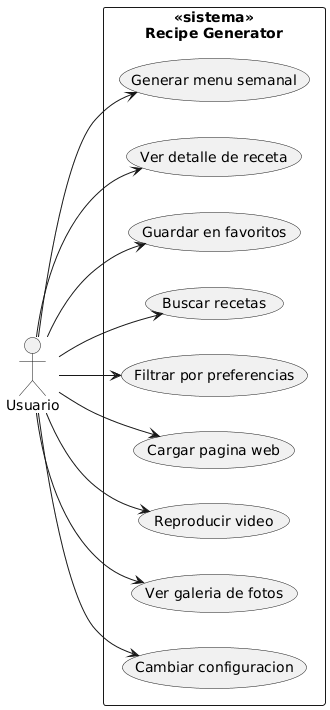
\includegraphics[width=0.40\textwidth]{diagrama_casos_uso.png}
\caption{Diagrama de casos de uso --- Recipe Generator. Elaboración propia.}
\label{fig:casosdeuso}
\end{figure}

\subsection{Diagrama de Clases (UML)}

El siguiente diagrama de clases describe el modelo de datos de la aplicación y las
relaciones entre sus entidades principales:

\begin{figure}[H]
\centering
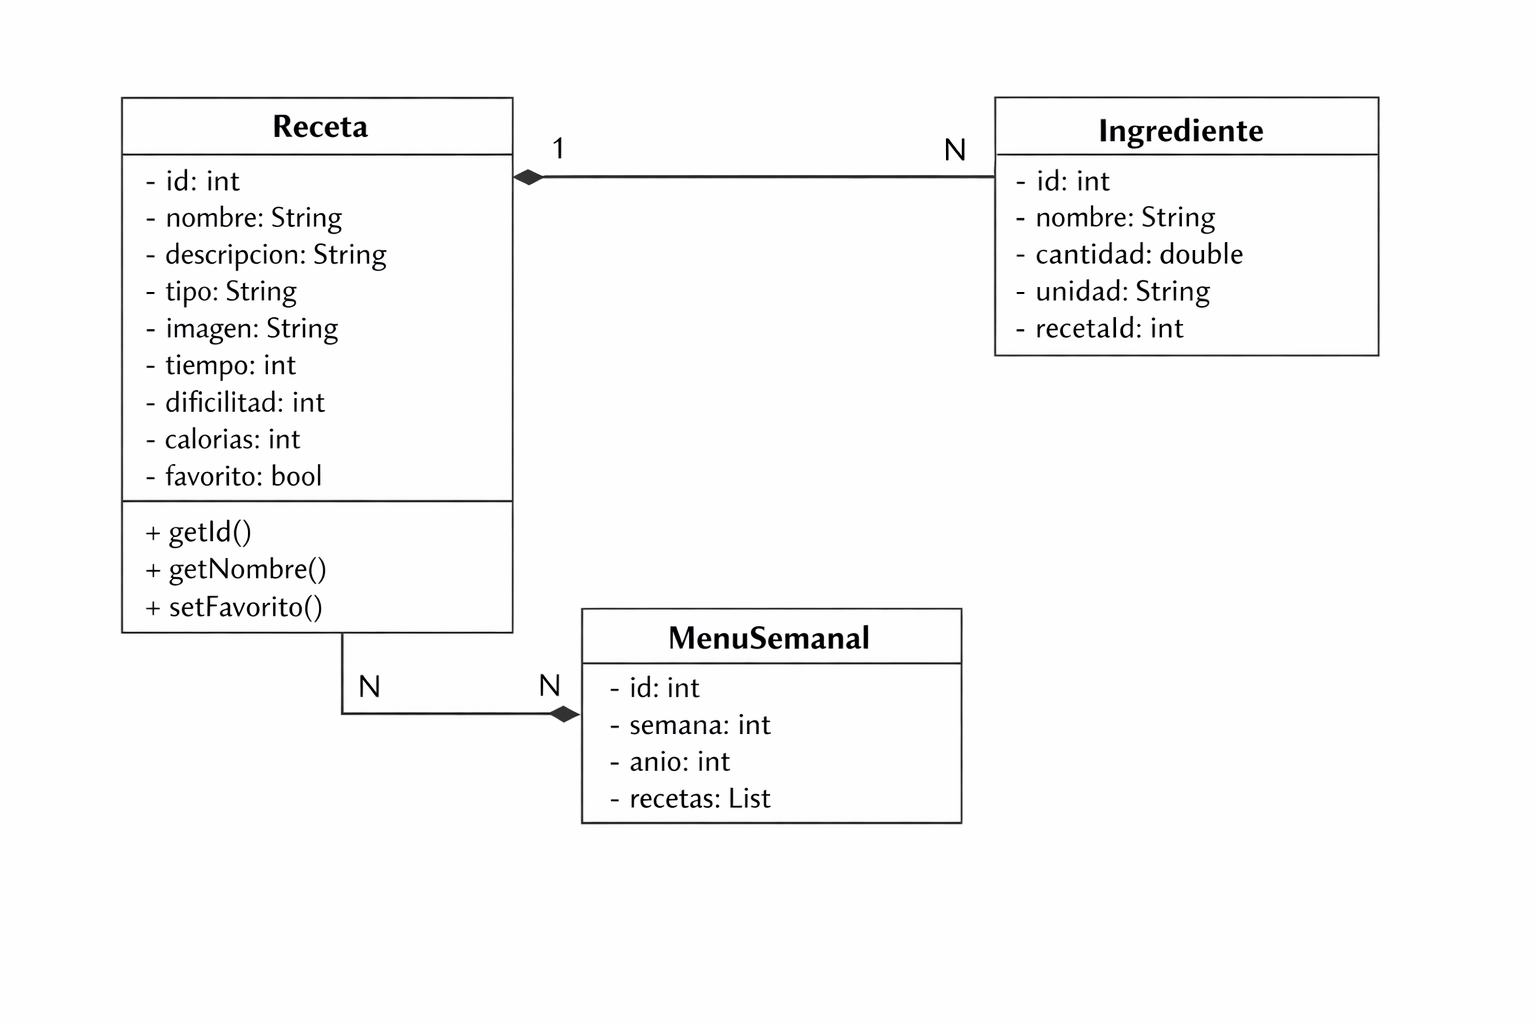
\includegraphics[width=\textwidth]{Diagrama-de-clases.png}
\caption{Diagrama de clases --- Modelo de datos. Elaboración propia.}
\label{fig:clases}
\end{figure}

\subsection{Arquitectura de la Aplicación}

La aplicación implementa el patrón arquitectónico MVVM (Model-View-ViewModel) sobre
el framework de Android \citep{smyth2017}, lo que garantiza una separación clara de
responsabilidades entre las capas de la aplicación:

\begin{itemize}
    \item \textbf{Capa View:} Actividades (\texttt{MainActivity}) y Fragmentos
    (\texttt{PerfilFragment}, \texttt{FotosFragment}, \texttt{VideoFragment},
    \texttt{WebFragment}, \texttt{BotonesFragment}). Gestionan la interfaz de usuario
    y los eventos del usuario.
    \item \textbf{Capa ViewModel:} Clases que exponen datos observables a la capa View
    mediante \texttt{LiveData}, desacoplando la lógica de negocio de la interfaz.
    \item \textbf{Capa Model:} Entidades Room (\texttt{Receta}, \texttt{Ingrediente},
    \texttt{MenuSemanal}) y DAOs que gestionan la persistencia local de datos.
    \item \textbf{Base de Datos:} Room Database sobre SQLite, con tablas para
    \texttt{RECETAS}, \texttt{INGREDIENTES}, \texttt{MENU\_SEMANAL} y \texttt{FAVORITOS}.
\end{itemize}

%+---------------------------------------------------------------+
\section{Diseño de la Interfaz Gráfica}

\subsection{Estructura General de Navegación}

La aplicación implementa una \texttt{BottomNavigationView} con cuatro opciones
principales (Inicio, Favoritos, Generador, Configuración). La pantalla principal contiene
dos fragmentos distribuidos horizontalmente: el fragmento izquierdo ocupa aproximadamente
el 30\% del ancho de pantalla y contiene el menú de opciones; el fragmento derecho ocupa
el 70\% restante y muestra el contenido correspondiente a la opción activa
\citep{androiddevelopers2024fragments}.

\subsection{Prototipo de Interfaz --- Vista Principal con Dos Fragmentos}

\begin{figure}[H]
\centering
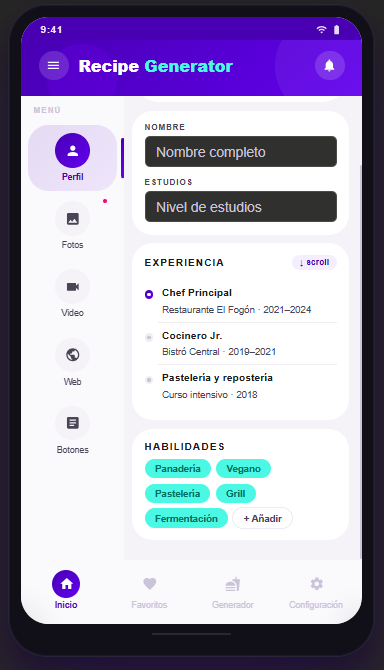
\includegraphics[width=0.35\textwidth]{Prototipo-de-interfaz.PNG}
\caption{Prototipo de interfaz --- Fragmentos izquierdo y derecho. Elaboración propia.}
\label{fig:prototipo}
\end{figure}

\subsection{Descripción de los Fragmentos}

\subsubsection{Fragmento Izquierdo --- Menú de Navegación}

Contiene cinco opciones presentadas como lista vertical: Perfil, Fotos, Video, Web y
Botones. Al seleccionar cualquier opción, el fragmento derecho actualiza su contenido
dinámicamente mediante la comunicación entre fragmentos a través de la actividad
contenedora (\texttt{MainActivity}). El fragmento usa un \texttt{LinearLayout} vertical
con botones o ítems de lista para cada opción.

\subsubsection{Fragmento Perfil}

Muestra la información personal de un integrante del equipo: foto de perfil
(\texttt{ImageView}), nombre completo, estudios realizados, experiencia profesional y
habilidades. Los campos de texto extensos están contenidos en un \texttt{ScrollView}
para optimizar el uso del espacio en pantalla, tal como indica la guía del proyecto.

\subsubsection{Fragmento Fotos}

Implementa un \texttt{RecyclerView} con scroll vertical que muestra una lista de
imágenes. Al seleccionar una imagen, se muestra su descripción en un \texttt{TextView}
inferior. Utiliza un adaptador personalizado (\texttt{ImageAdapter}) que gestiona la
lista de ítems con imagen y texto.

\subsubsection{Fragmento Video}

Integra un \texttt{VideoView} de Android con sus controles nativos de reproducción
(play, pause, barra de progreso). El video puede ser un recurso local almacenado en la
carpeta \texttt{raw} de los recursos o una URL de video.

\subsubsection{Fragmento Web}

Contiene un \texttt{EditText} para que el usuario ingrese una URL, un \texttt{Button}
para confirmar la navegación y un \texttt{WebView} que carga y renderiza la página web
solicitada. Se configura con soporte para JavaScript y carga de contenido HTTPS.

\subsubsection{Fragmento Botones}

Demuestra el uso de diferentes tipos de controles de botón disponibles en Android:
\texttt{Button} estándar, \texttt{ImageButton}, \texttt{FloatingActionButton},
\texttt{ToggleButton} y \texttt{CheckBox}. Cada botón tiene un evento \texttt{onClick}
asociado que muestra un mensaje \texttt{Toast} o actualiza un \texttt{TextView} con el
resultado de la interacción.

\subsection{Paleta de Colores y Especificaciones de Diseño}

La paleta de colores de Recipe Generator se basa en Material Design~3
\citep{googlematerial2024}, definiendo colores primarios, secundarios y terciarios que
garantizan coherencia visual, accesibilidad y contraste adecuado en toda la interfaz
de la aplicación.

\begin{table}[H]
\caption{Paleta de colores --- Material Design~3}
\label{tab:colores}
\begin{tabularx}{\textwidth}{@{}llX@{}}
\toprule
\textbf{Elemento}   & \textbf{Color Hex}  & \textbf{Uso} \\
\midrule
Color Primario      & \texttt{\#6200EE}   & Botones principales, BottomNavigation activa \\
Color Secundario    & \texttt{\#03DAC6}   & Acciones secundarias, indicadores \\
Color Terciario     & \texttt{\#FF0081}   & Alertas, favoritos, destacados \\
Fondo               & \texttt{\#FFFFFF}   & Fondo general de la app \\
Texto principal     & \texttt{\#000000}   & Títulos y contenido principal \\
Texto secundario    & \texttt{\#666666}   & Subtítulos y metadata \\
\bottomrule
\end{tabularx}
\end{table}

La figura~\ref{fig:paleta} presenta la representación visual de la paleta de colores
aplicada al sistema de diseño de la aplicación, mostrando cómo cada tono se integra
con los componentes de la interfaz siguiendo los lineamientos de Material Design~3.

\begin{figure}[H]
\centering
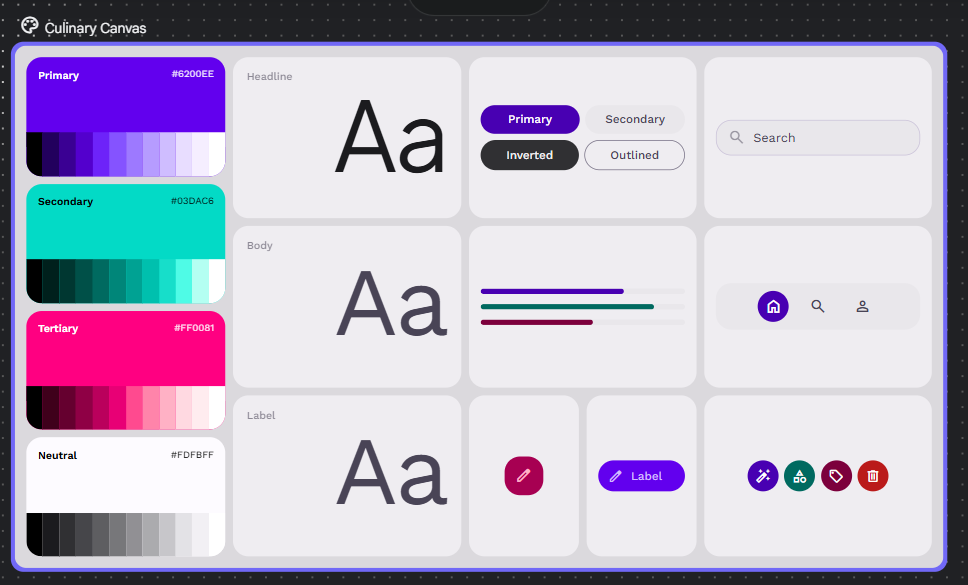
\includegraphics[width=0.90\textwidth]{Paleta-de-Colores.PNG}
\caption{Paleta de colores aplicada --- Material Design~3. Elaboración propia.}
\label{fig:paleta}
\end{figure}

La figura~\ref{fig:disenio} muestra el diseño completo de las vistas principales de
Recipe Generator, ilustrando la distribución de componentes, la navegación entre
pantallas y la aplicación consistente de la paleta de colores y la tipografía
definidas para la aplicación.

\begin{figure}[H]
\centering
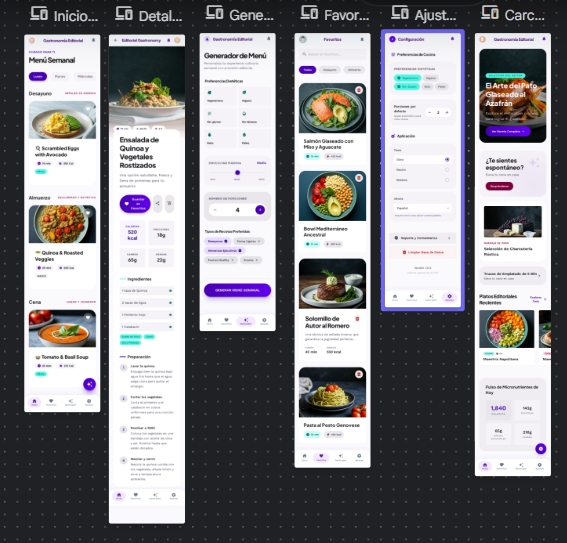
\includegraphics[width=0.90\textwidth]{Disenio.PNG}
\caption{Diseño de vistas principales --- Recipe Generator. Elaboración propia.}
\label{fig:disenio}
\end{figure}

\subsection{Estructura de Pantallas}

A continuación se describe la estructura detallada de cada pantalla principal de la
aplicación Recipe Generator y sus componentes de interfaz asociados.

\subsubsection{Pantalla Principal (\texttt{MainActivity})}
\begin{itemize}
    \item \texttt{BottomNavigationView} con 4 opciones principales (Inicio, Favoritos,
    Generador, Configuración).
    \item Estructura de navegación para Fragments.
\end{itemize}

\subsubsection{Home --- Menú Semanal}
\begin{itemize}
    \item \texttt{TabLayout} con 7 tabs (Lunes a Domingo).
    \item \texttt{ViewPager2} para navegar por días.
    \item 3 \texttt{CardViews} por día: Desayuno, Almuerzo y Comida.
    \item Cada Card: Imagen, Nombre, Favorito, Tiempo, Calorías, Dificultad.
\end{itemize}

\subsubsection{Detalle de Receta}
\begin{itemize}
    \item Hero Image.
    \item Info Nutricional: Calorías, proteínas, carbohidratos, grasas.
    \item Lista de ingredientes.
    \item Pasos de preparación.
    \item Rating y acciones (Guardar, Compartir, Lista de compras).
\end{itemize}

\subsubsection{Favoritos}
\begin{itemize}
    \item Lista de recetas guardadas.
    \item Filtros por tipo de comida.
    \item Búsqueda y opción de eliminar.
\end{itemize}

\subsubsection{Generador Personalizado}
\begin{itemize}
    \item Preferencias dietéticas (Vegetariano, Vegano, Keto, etc.).
    \item Slider de dificultad.
    \item Selector de porciones.
    \item Botón principal: \textbf{``GENERAR MENÚ SEMANAL''}.
\end{itemize}

\subsubsection{Configuración}
\begin{itemize}
    \item Preferencias por defecto.
    \item Tema (Light/Dark/System).
    \item Idioma.
    \item Gestión de base de datos.
\end{itemize}

\subsection{Modelo de Datos}

La siguiente tabla describe las entidades del modelo de datos de la aplicación y sus
atributos principales, los cuales son gestionados mediante Room Database sobre SQLite
\citep{androiddevelopers2024room}.

\begin{table}[H]
\caption{Entidades del modelo de datos --- Recipe Generator}
\label{tab:modelodatos}
\begin{tabularx}{\textwidth}{@{}lX@{}}
\toprule
\textbf{Entidad} & \textbf{Atributos} \\
\midrule
\texttt{Recipe}      & \texttt{id}, nombre, descripcion, tipo, imagen, tiempo, dificultad,
                       calorias, macros, pasos, dia, favorito \\[4pt]
\texttt{Ingredient}  & nombre, cantidad, unidad \\[4pt]
\texttt{MenuSemanal} & semana, año, recetas asociadas \\
\bottomrule
\end{tabularx}
\end{table}

\begin{center}
\textbf{\Large Conclusión}
\end{center}
{\normalsize\setlength{\parskip}{6pt}

El desarrollo de esta entrega previa permitió consolidar los fundamentos del módulo
de Herramientas de Programación Móvil~I mediante el diseño y planificación de
Recipe Generator, una aplicación Android nativa desarrollada en Kotlin con Android
Studio bajo los lineamientos de Material Design~3 \citep{googlematerial2024}.

La definición de objetivos, el análisis de requerimientos y la especificación UML
establecieron un alcance claro y documentado, identificando los componentes clave del
framework Android: actividades, fragmentos, intents, layouts y el patrón MVVM,
garantizando una arquitectura sólida y mantenible \citep{smyth2017}.

El diseño de la interfaz gráfica, los prototipos visuales y la descripción de la
estructura de pantallas dejaron una hoja de ruta concreta para las siguientes fases
de desarrollo, donde todo lo planificado se materializará en código funcional
\citep{robledo2017}.
}

% Referencias Entrega 1
\renewcommand{\refname}{\large\textbf{Referencias}}
\bibliography{mibibliografia}

%+---------------------------------------------------------------+
%+---------------------------------------------------------------+
%          ENTREGA PROYECTO 2 — ESCENARIO 5
%+---------------------------------------------------------------+
%+---------------------------------------------------------------+

\newpage
\section{Entrega proyecto 2 --- Escenario 5}

\begin{center}
\textbf{\large Introducción}
\end{center}

En esta segunda entrega se presenta la implementación funcional de Recipe Generator, la
aplicación móvil Android diseñada en la primera entrega. Se materializaron en código Kotlin
las actividades, fragmentos, interfaces gráficas, identificadores de vistas, variables de
estado y eventos de interacción propuestos inicialmente, utilizando Jetpack Compose como
sistema de interfaz gráfica y manteniendo la compatibilidad con los lineamientos de las
lecturas fundamentales del curso (LF1 a LF8).

El documento detalla las actividades y fragmentos
(sección~\ref{sec:actividadesfragmentos}), la creación de interfaces
(sección~\ref{sec:creacioninterfaz}), la asignación de identificadores
(sección~\ref{sec:identificadores}), la definición de variables
(sección~\ref{sec:variables}) y la identificación de eventos
(sección~\ref{sec:eventos}).

\newpage
%+---------------------------------------------------------------+
\subsection{Actividades y Fragmentos que utiliza la aplicación}
\label{sec:actividadesfragmentos}

La aplicación Recipe Generator está desarrollada en Kotlin con Jetpack Compose (el
estándar oficial de Android desde 2021), lo que reemplaza los layouts XML clásicos por
composables declarativos. A continuación se describen todas las Actividades y Fragmentos
que conforman la aplicación.

\subsubsection{Actividades}

\textbf{MainActivity}

\noindent\textbf{Archivo:} \texttt{MainActivity.kt}

\noindent\textbf{Función:} Es el punto de entrada de la aplicación. Se encarga de
gestionar el flujo de autenticación del usuario, aplicar el tema visual (claro/oscuro)
según las preferencias guardadas en DataStore, y mostrar la pantalla correspondiente
según el estado de sesión: pantalla de carga, pantalla de autenticación, pantalla de
bienvenida o el shell principal de la app.

Contiene el \texttt{FragmentContainerView} definido en \texttt{activity\_main.xml}, que
actúa como contenedor del grafo de navegación (\texttt{main\_nav\_graph.xml}). Todos los
fragmentos de la app se renderizan dentro de esta actividad.

\noindent\textbf{Responsabilidades principales:}
\begin{itemize}[nosep]
    \item Solicitar permisos de notificaciones al iniciar (Android 13+).
    \item Observar el estado de autenticación mediante \texttt{AuthViewModel}.
    \item Sincronizar datos locales con Firestore al hacer login y al recuperar
    conectividad.
    \item Inyectar el tema oscuro/claro desde las preferencias del usuario.
\end{itemize}

\begin{figure}[H]
\centering
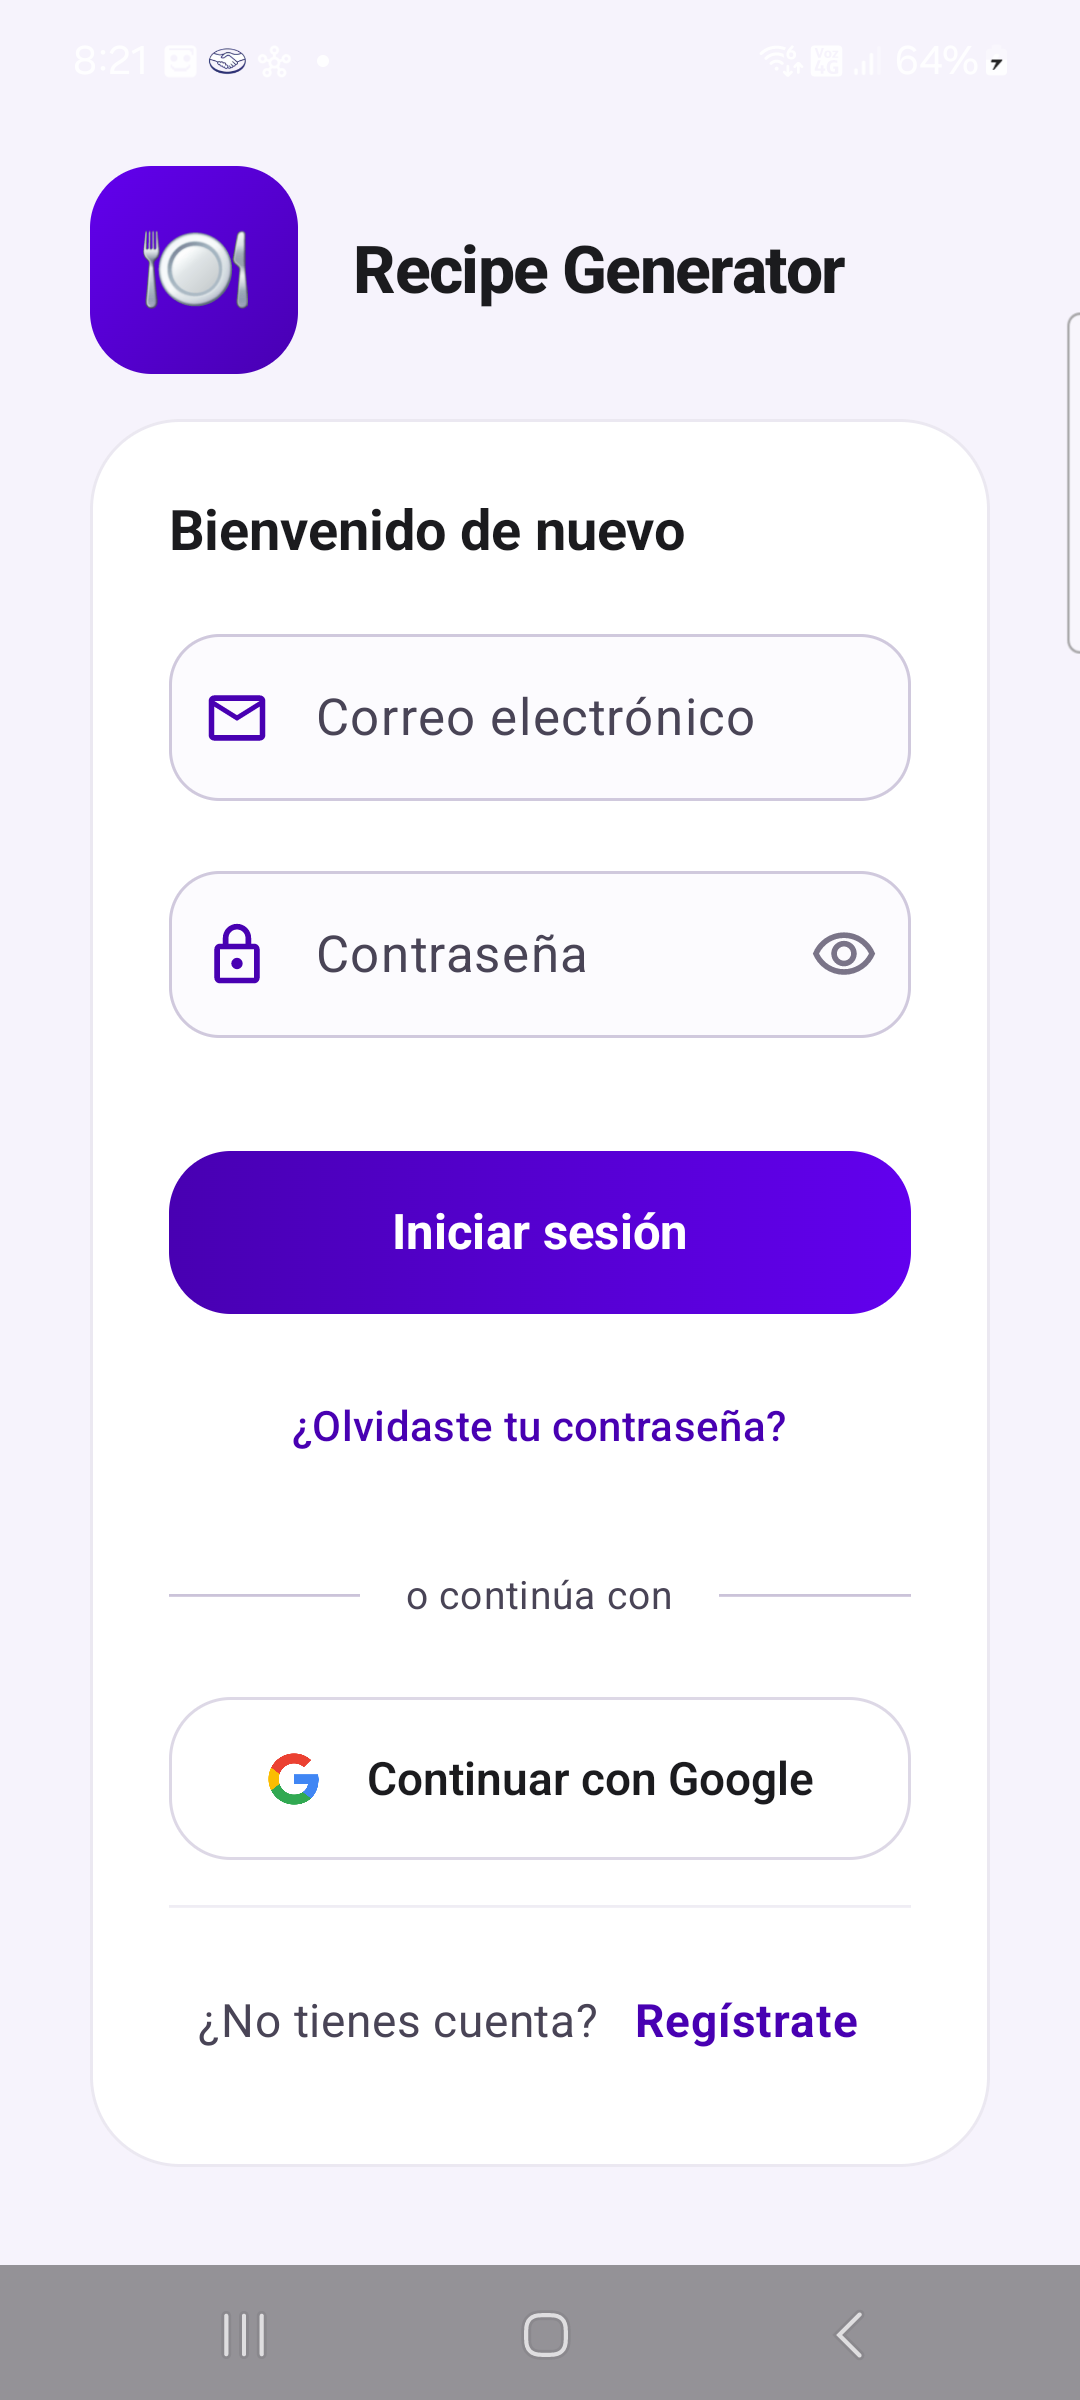
\includegraphics[width=0.30\textwidth]{screenshot_mainactivity.png}
\caption{Captura de pantalla --- MainActivity mostrando el shell principal con la barra
de navegación inferior activa. Elaboración propia.}
\label{fig:ss_mainactivity}
\end{figure}

\textbf{RecipeDetailActivity}

\noindent\textbf{Archivo:} \texttt{presentation/detail/RecipeDetailActivity.kt}

\noindent\textbf{Función:} Segunda actividad de la aplicación. Es lanzada desde
\texttt{HomeFragment} y \texttt{FavoritesFragment} mediante un \texttt{Intent} que
transporta el identificador único de la receta (\texttt{EXTRA\_RECIPE\_ID}). Muestra el
detalle completo de una receta: nombre, descripción, ingredientes, pasos de preparación,
botón de favorito y enlace a video de YouTube.

\noindent\textbf{Responsabilidades principales:}
\begin{itemize}[nosep]
    \item Recibir el ID de receta desde el \texttt{Intent} con
    \texttt{getStringExtra(EXTRA\_RECIPE\_ID)}.
    \item Cargar el detalle de la receta usando \texttt{GetRecipeDetailUseCase}.
    \item Observar y actualizar el estado de favorito en tiempo real.
    \item Gestionar la resolución del video de YouTube mediante
    \texttt{EnsureRecipeVideoUseCase}.
    \item Retornar a la pantalla anterior usando el back stack nativo de Android.
\end{itemize}

\begin{figure}[H]
\centering
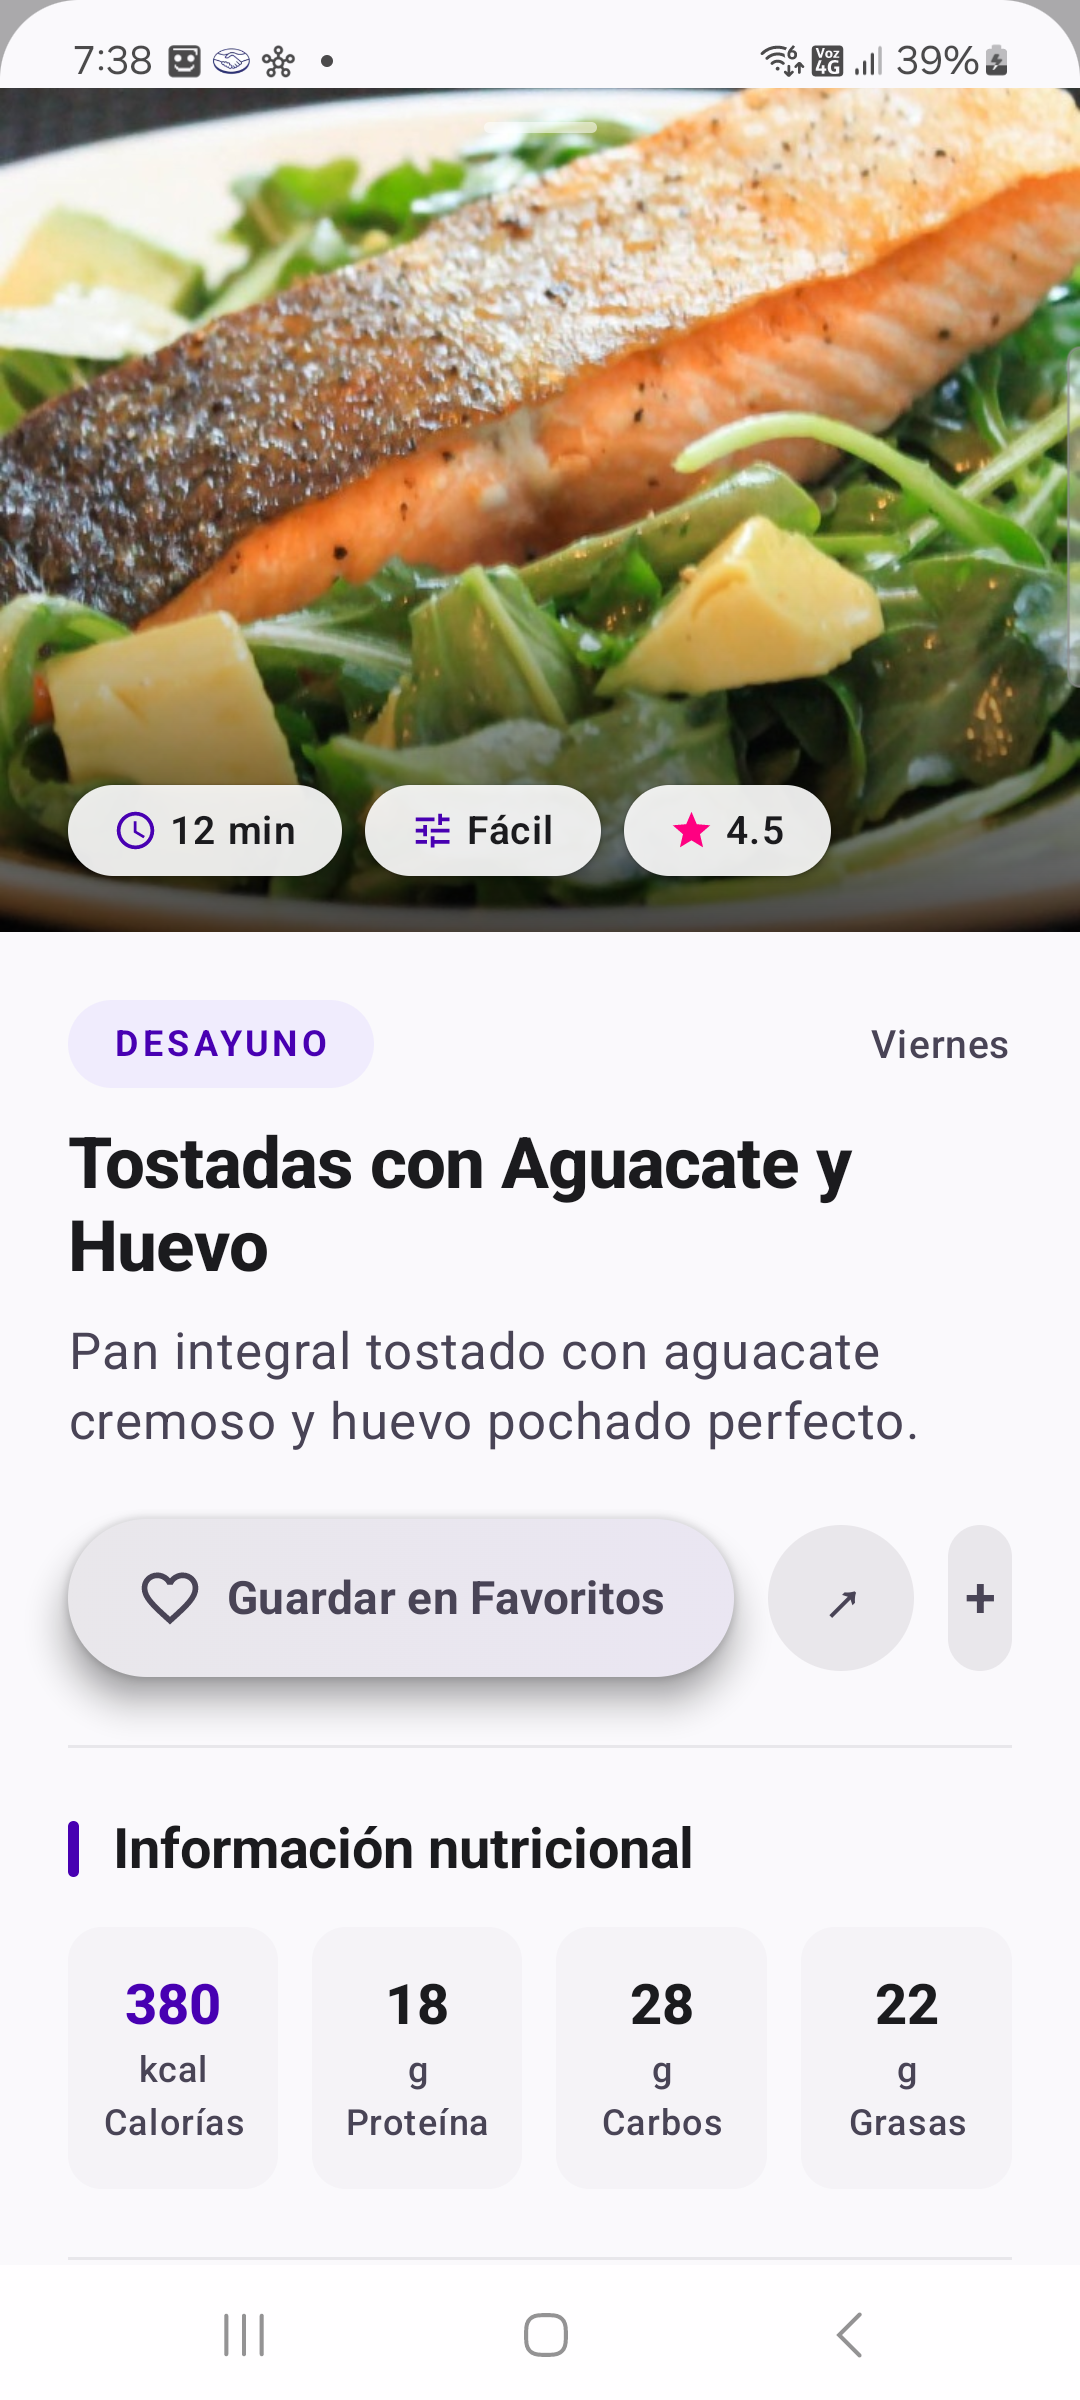
\includegraphics[width=0.30\textwidth]{screenshot_recipedetail.png}
\caption{Captura de pantalla --- RecipeDetailActivity mostrando el detalle completo de
una receta con imagen, ingredientes y pasos. Elaboración propia.}
\label{fig:ss_recipedetail}
\end{figure}

\subsubsection{Fragmentos}

La aplicación usa un Fragment base abstracto del que heredan todos los demás.

\textbf{ComposeScreenFragment (clase base abstracta)}

\noindent\textbf{Archivo:} \texttt{presentation/navigation/ComposeScreenFragment.kt}

\noindent\textbf{Función:} Fragment base que todos los demás fragmentos extienden. En su
método \texttt{onCreateView()} crea un \texttt{ComposeView} como vista raíz, configura el
tema visual leyendo las preferencias del usuario desde DataStore y delega el contenido
visual al método abstracto \texttt{ScreenContent()}, que cada subclase implementa con su
propio composable.

También provee el método utilitario \texttt{navigateToTopLevel(index)} para que cada
fragment pueda navegar entre los destinos principales usando el \texttt{NavController}.

\textbf{HomeFragment}

\noindent\textbf{Archivo:} \texttt{presentation/home/HomeFragment.kt}

\noindent\textbf{Función:} Pantalla principal de la aplicación. Muestra el menú semanal de
recetas organizadas por día (Lunes a Domingo) mediante pestañas. El usuario puede
seleccionar el día activo y ver las recetas correspondientes. Permite marcar recetas como
favoritas directamente desde la lista y navegar al detalle de cualquier receta.

\noindent\textbf{Acciones desde este fragmento:}
\begin{itemize}[nosep]
    \item Lanzar \texttt{RecipeDetailActivity} con el ID de la receta seleccionada.
    \item Navegar al \texttt{LeftMenuFragment} (sistema de dos paneles) al tocar el ícono
    de perfil.
\end{itemize}

\begin{figure}[H]
\centering
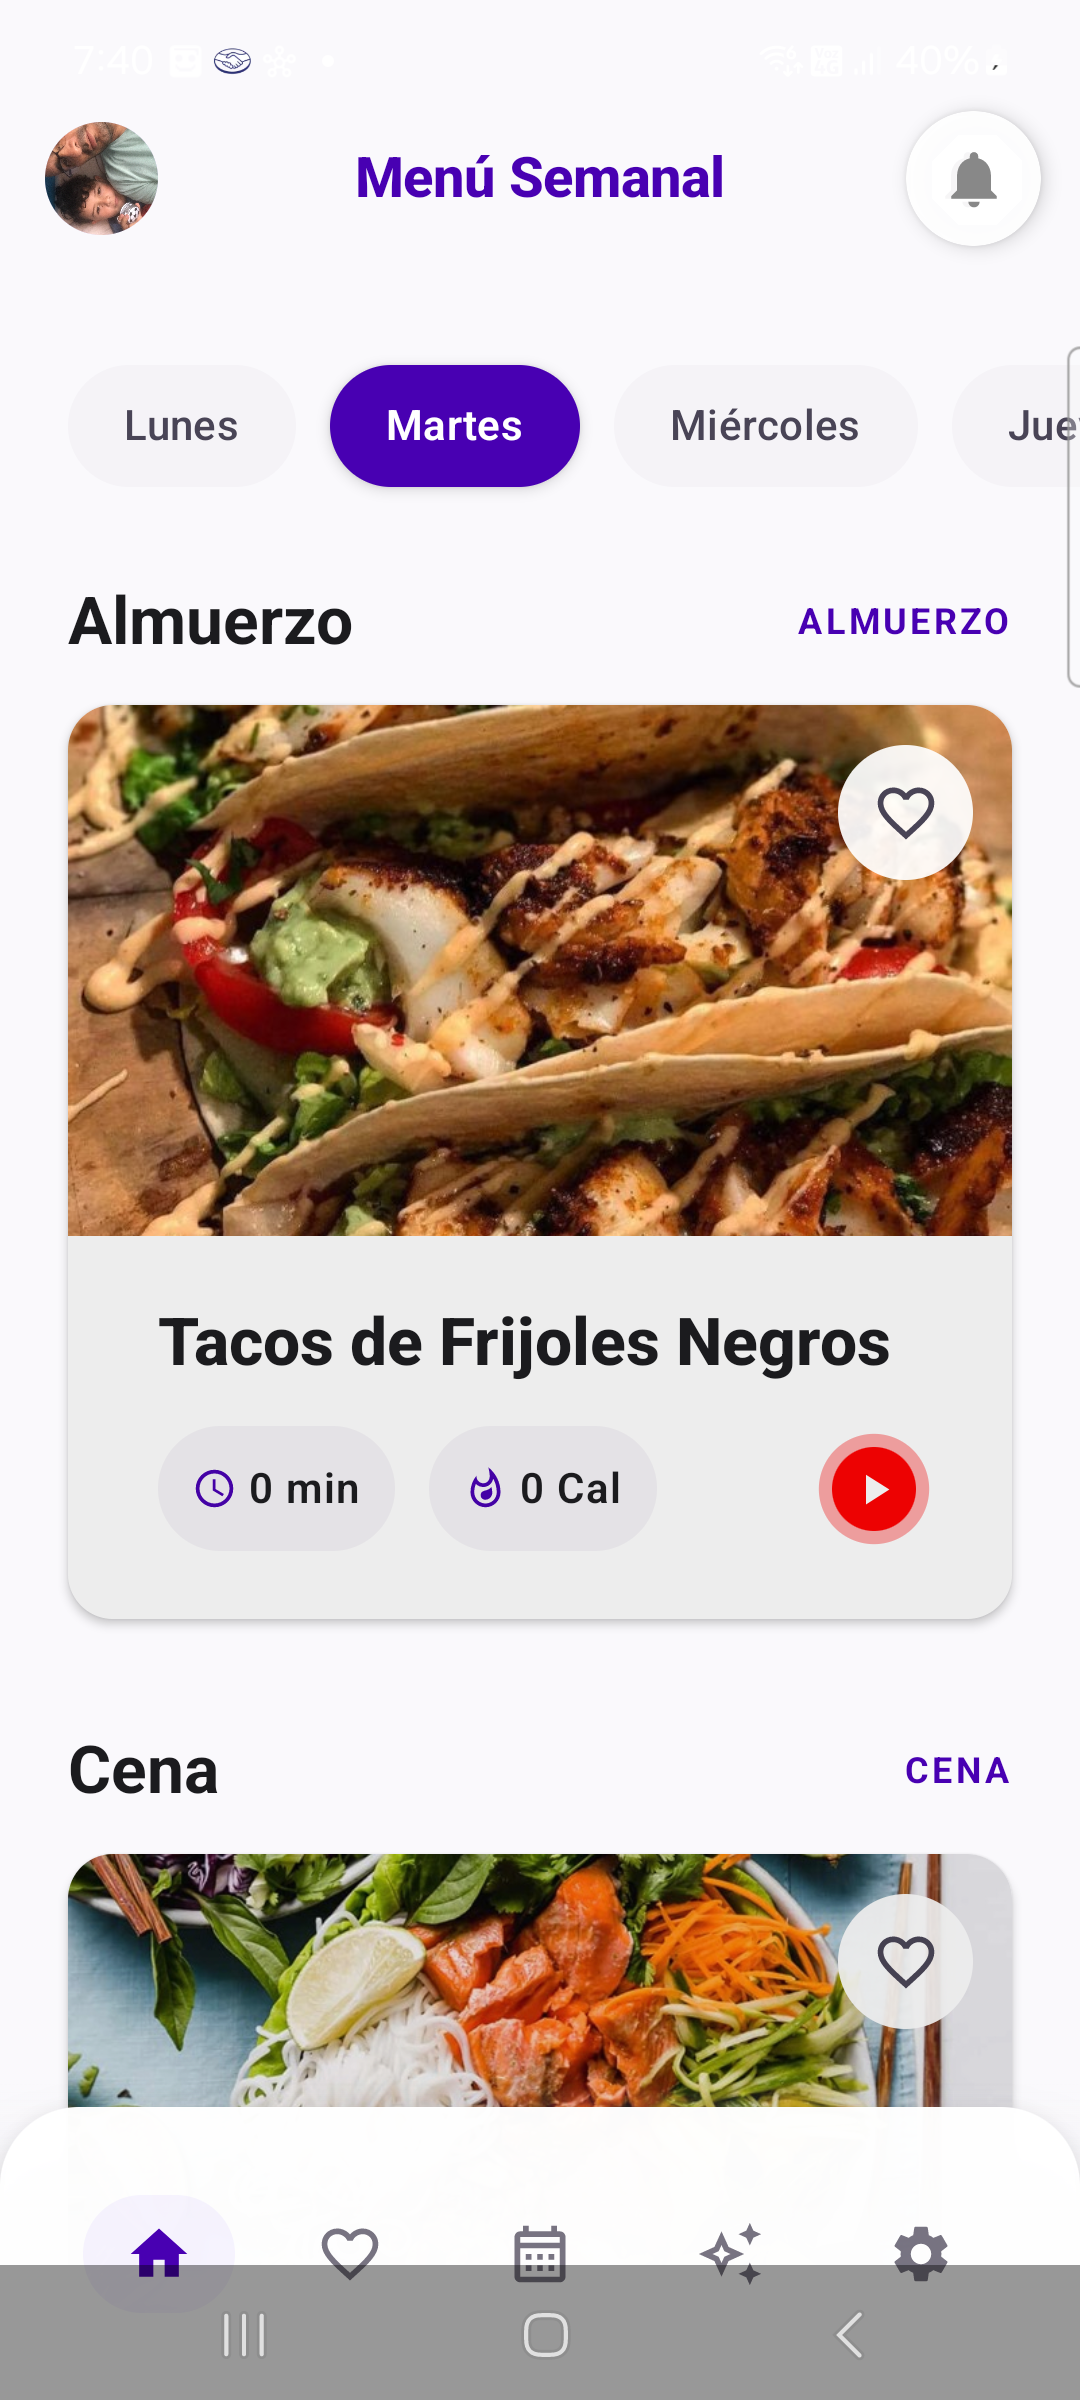
\includegraphics[width=0.30\textwidth]{screenshot_home.png}
\caption{Captura de pantalla --- HomeFragment con el menú semanal organizado por pestañas
de días y tarjetas de recetas. Elaboración propia.}
\label{fig:ss_home}
\end{figure}

\textbf{FavoritesFragment}

\noindent\textbf{Archivo:} \texttt{presentation/favorites/FavoritesFragment.kt}

\noindent\textbf{Función:} Muestra la lista de recetas marcadas como favoritas por el
usuario. Incluye un campo de búsqueda por texto y filtros por categoría (Desayuno,
Almuerzo, Cena, etc.). Permite eliminar favoritos y navegar al detalle de cualquier
receta.

\begin{figure}[H]
\centering
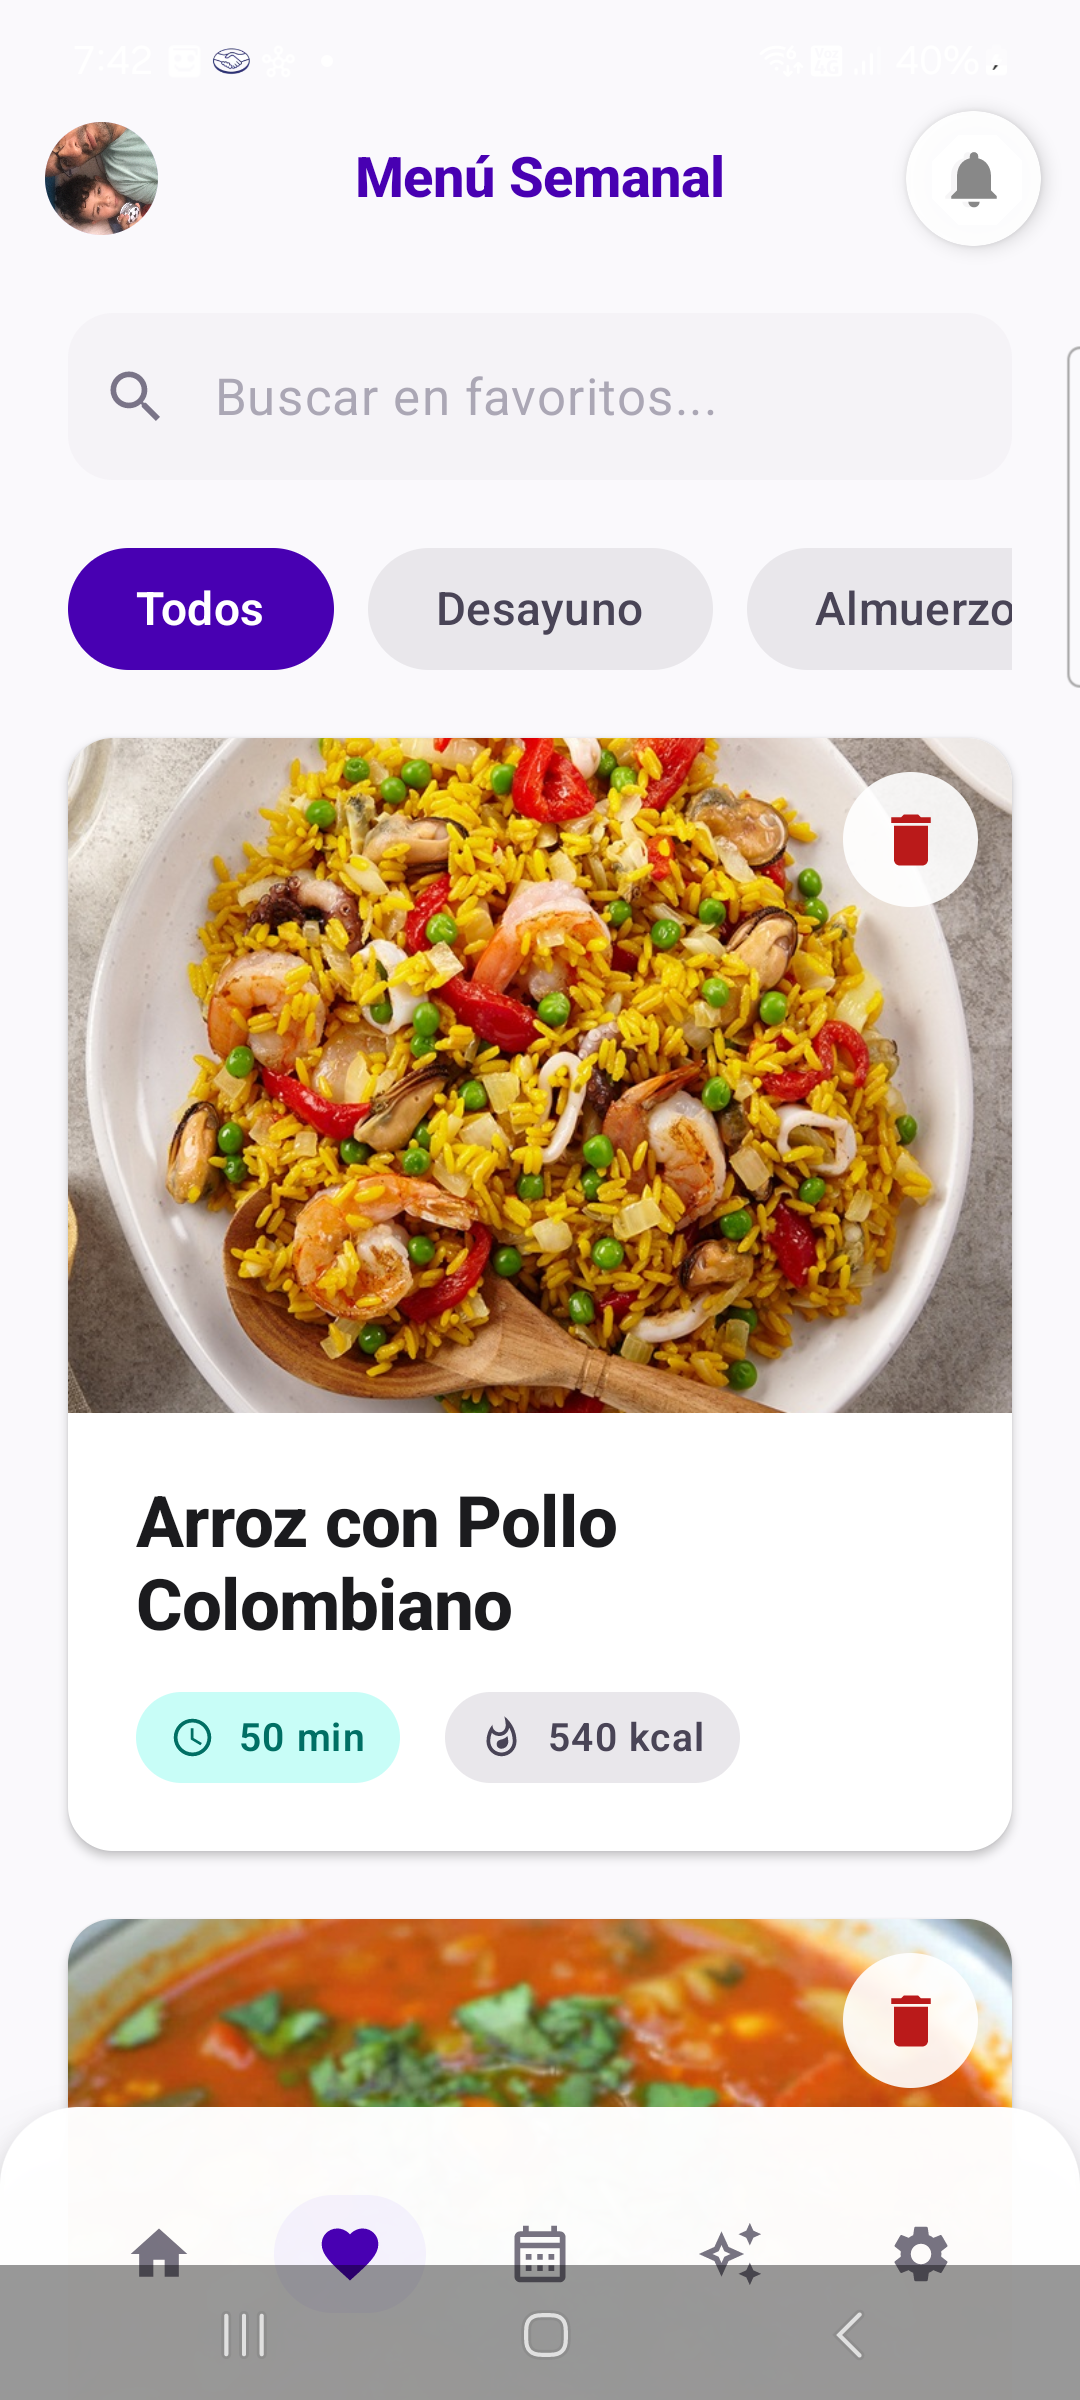
\includegraphics[width=0.30\textwidth]{screenshot_favorites.png}
\caption{Captura de pantalla --- FavoritesFragment con campo de búsqueda, filtros por
categoría y lista de recetas favoritas. Elaboración propia.}
\label{fig:ss_favorites}
\end{figure}

\textbf{MenuGeneratorFragment}

\noindent\textbf{Archivo:} \texttt{presentation/generator/MenuGeneratorFragment.kt}

\noindent\textbf{Función:} Pantalla del generador de menús con inteligencia artificial
(Google Gemini). El usuario configura parámetros como tipo de dieta (vegetariana, vegana,
etc.), nivel de dificultad máximo, número de porciones y tipos de receta deseados. Al
confirmar, la IA genera un plan semanal completo que se guarda en la base de datos local.

\begin{figure}[H]
\centering
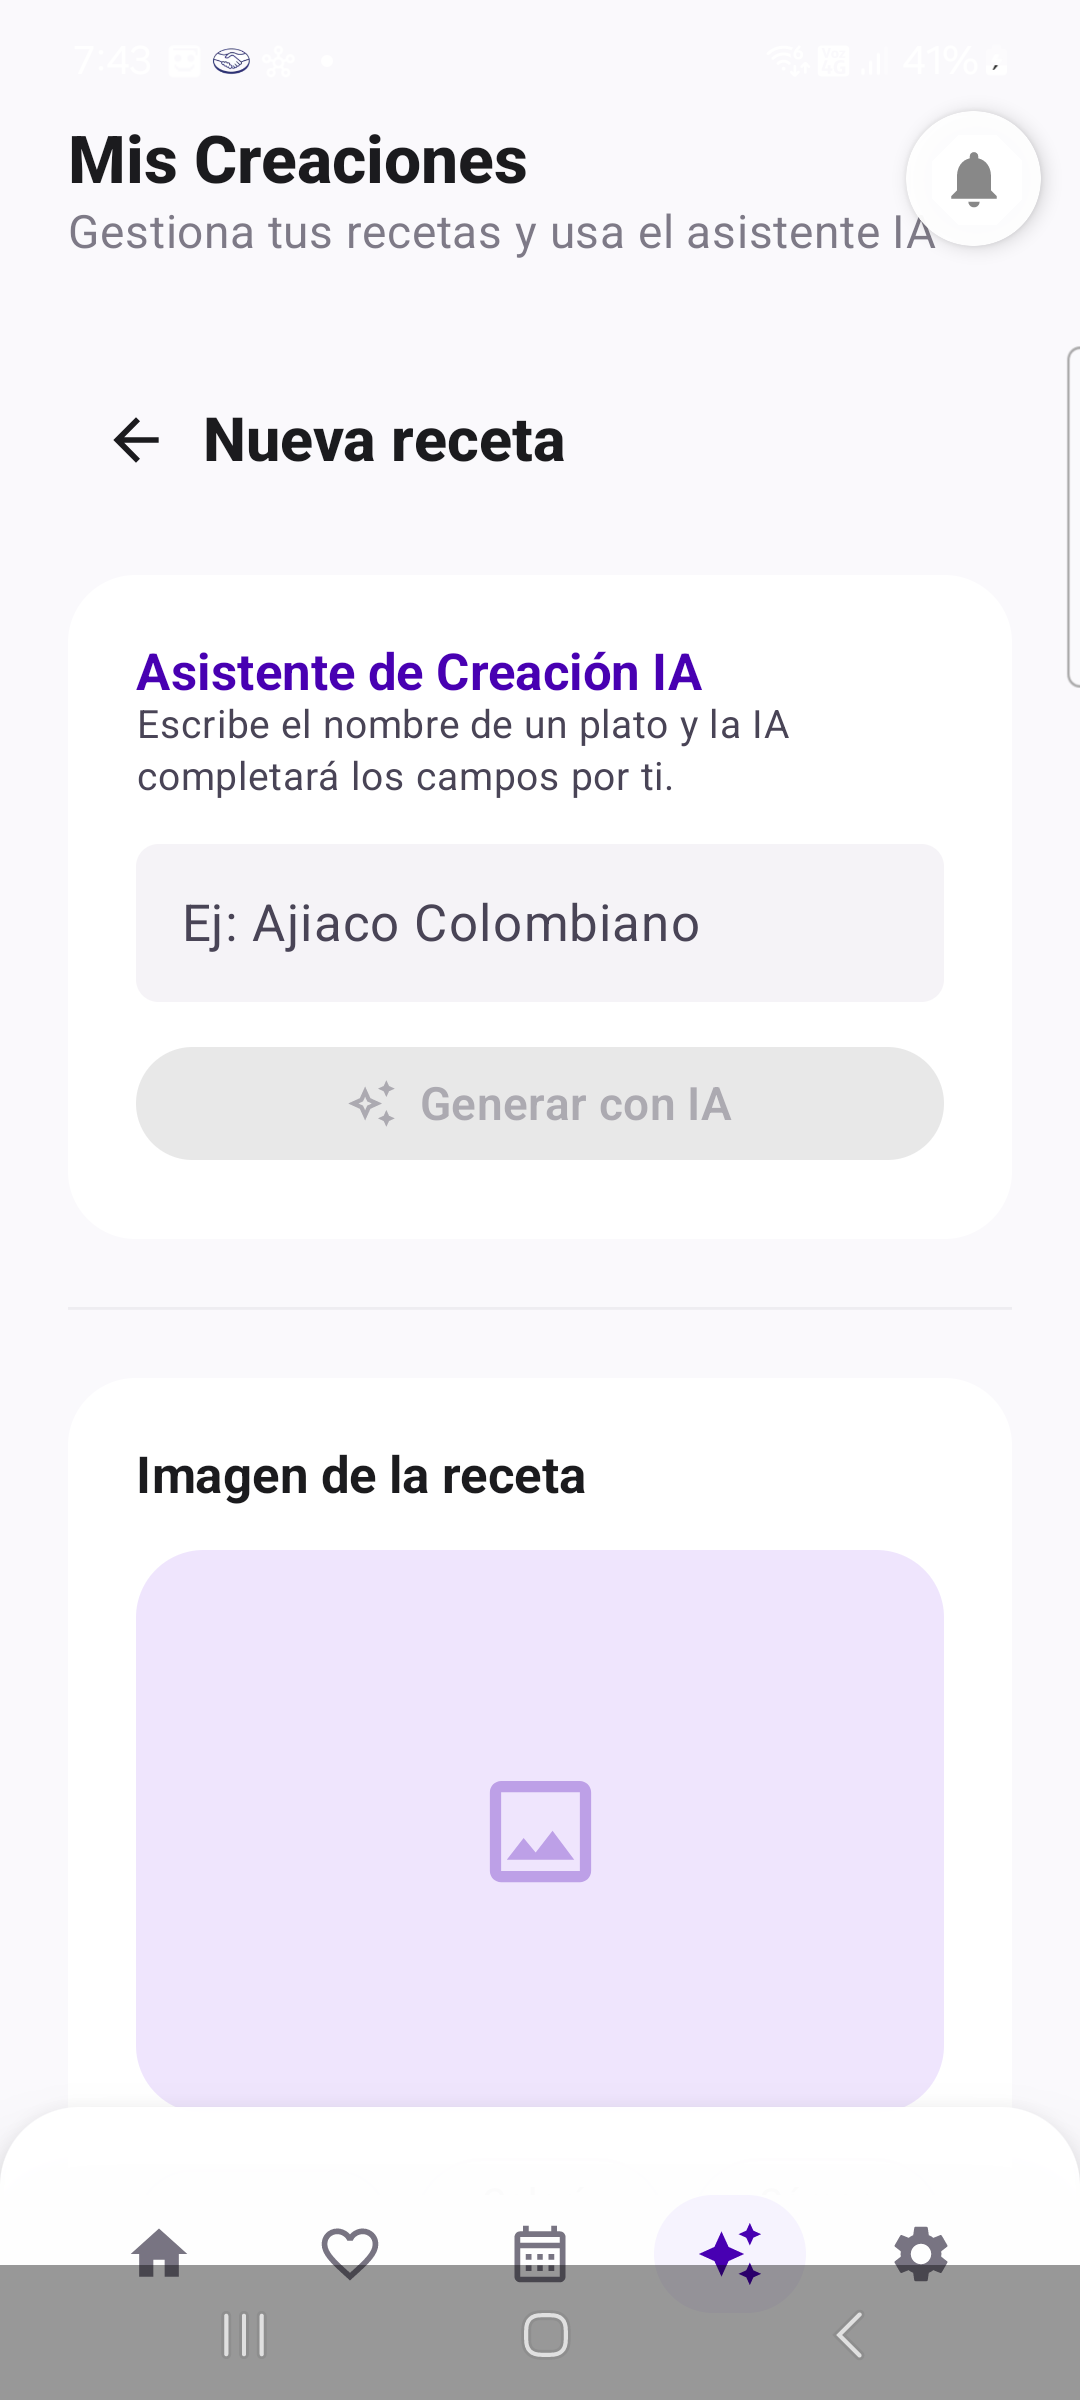
\includegraphics[width=0.30\textwidth]{screenshot_generator.png}
\caption{Captura de pantalla --- MenuGeneratorFragment con controles de configuración del
generador de menús con IA. Elaboración propia.}
\label{fig:ss_generator}
\end{figure}

\textbf{SettingsFragment}

\noindent\textbf{Archivo:} \texttt{presentation/settings/SettingsFragment.kt}

\noindent\textbf{Función:} Pantalla de configuración de la aplicación. Permite al usuario
seleccionar el tema visual (claro/oscuro), el idioma de la interfaz, las dietas
predeterminadas y el número de porciones por defecto. También contiene la opción de cerrar
sesión, que limpia los datos locales del usuario y retorna a la pantalla de autenticación.

\begin{figure}[H]
\centering
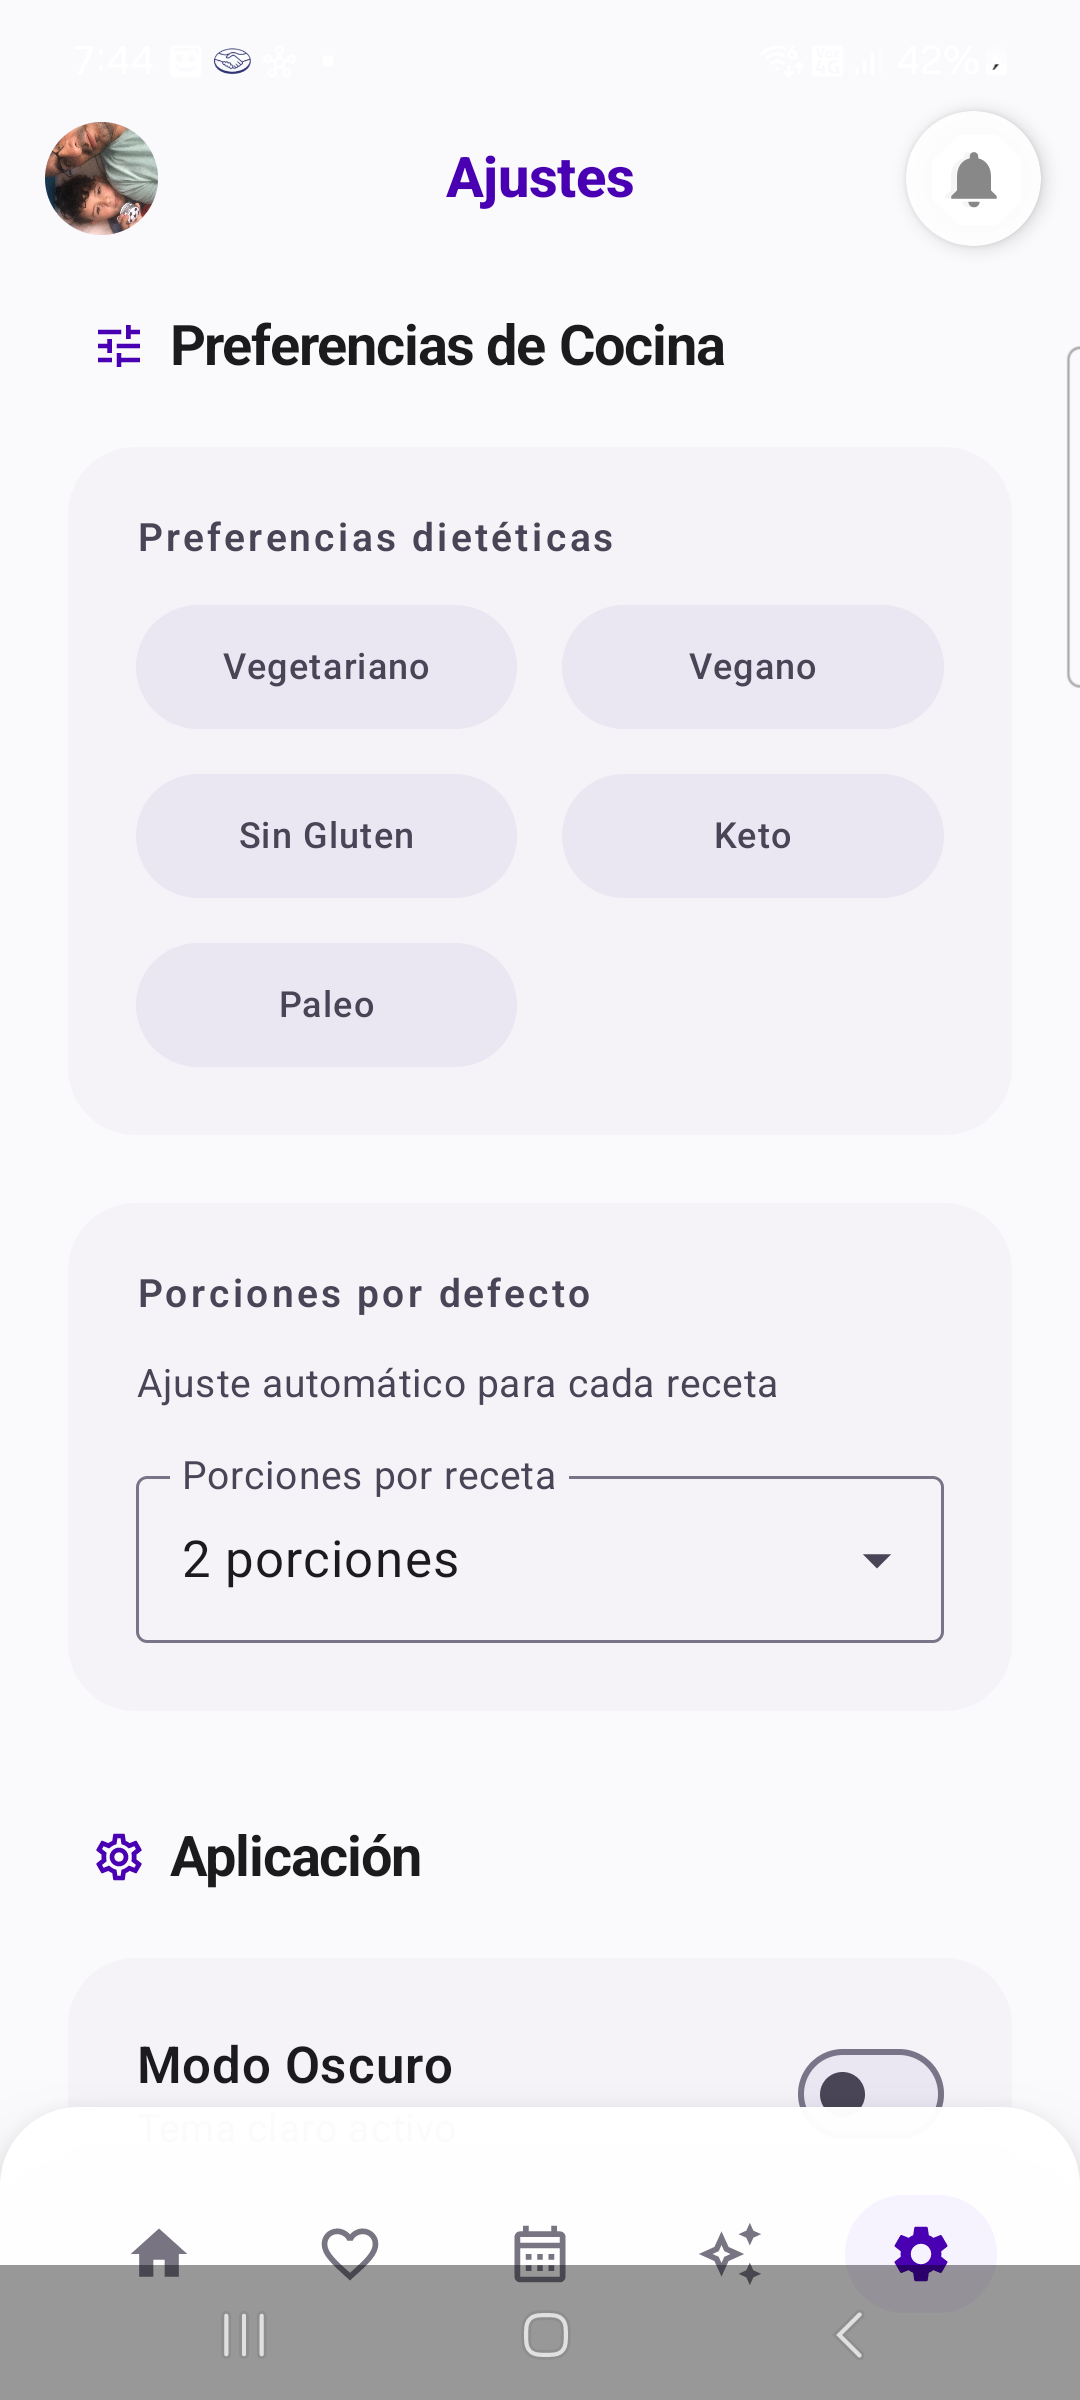
\includegraphics[width=0.30\textwidth]{screenshot_settings.png}
\caption{Captura de pantalla --- SettingsFragment con opciones de tema, idioma, dietas y
porciones predeterminadas. Elaboración propia.}
\label{fig:ss_settings}
\end{figure}

\textbf{GlobalRecipeSearchFragment}

\noindent\textbf{Archivo:} \texttt{presentation/ui/GlobalRecipeSearchFragment.kt}

\noindent\textbf{Función:} Fragment que implementa la búsqueda global de recetas
combinando la base de datos local (Room) con fuentes externas (TheMealDB API). A
diferencia de los demás fragmentos, infla un layout XML
(\texttt{fragment\_global\_recipe\_search.xml}) que contiene un \texttt{ComposeView},
demostrando la integración híbrida entre vistas XML tradicionales y Jetpack Compose.

\begin{figure}[H]
\centering
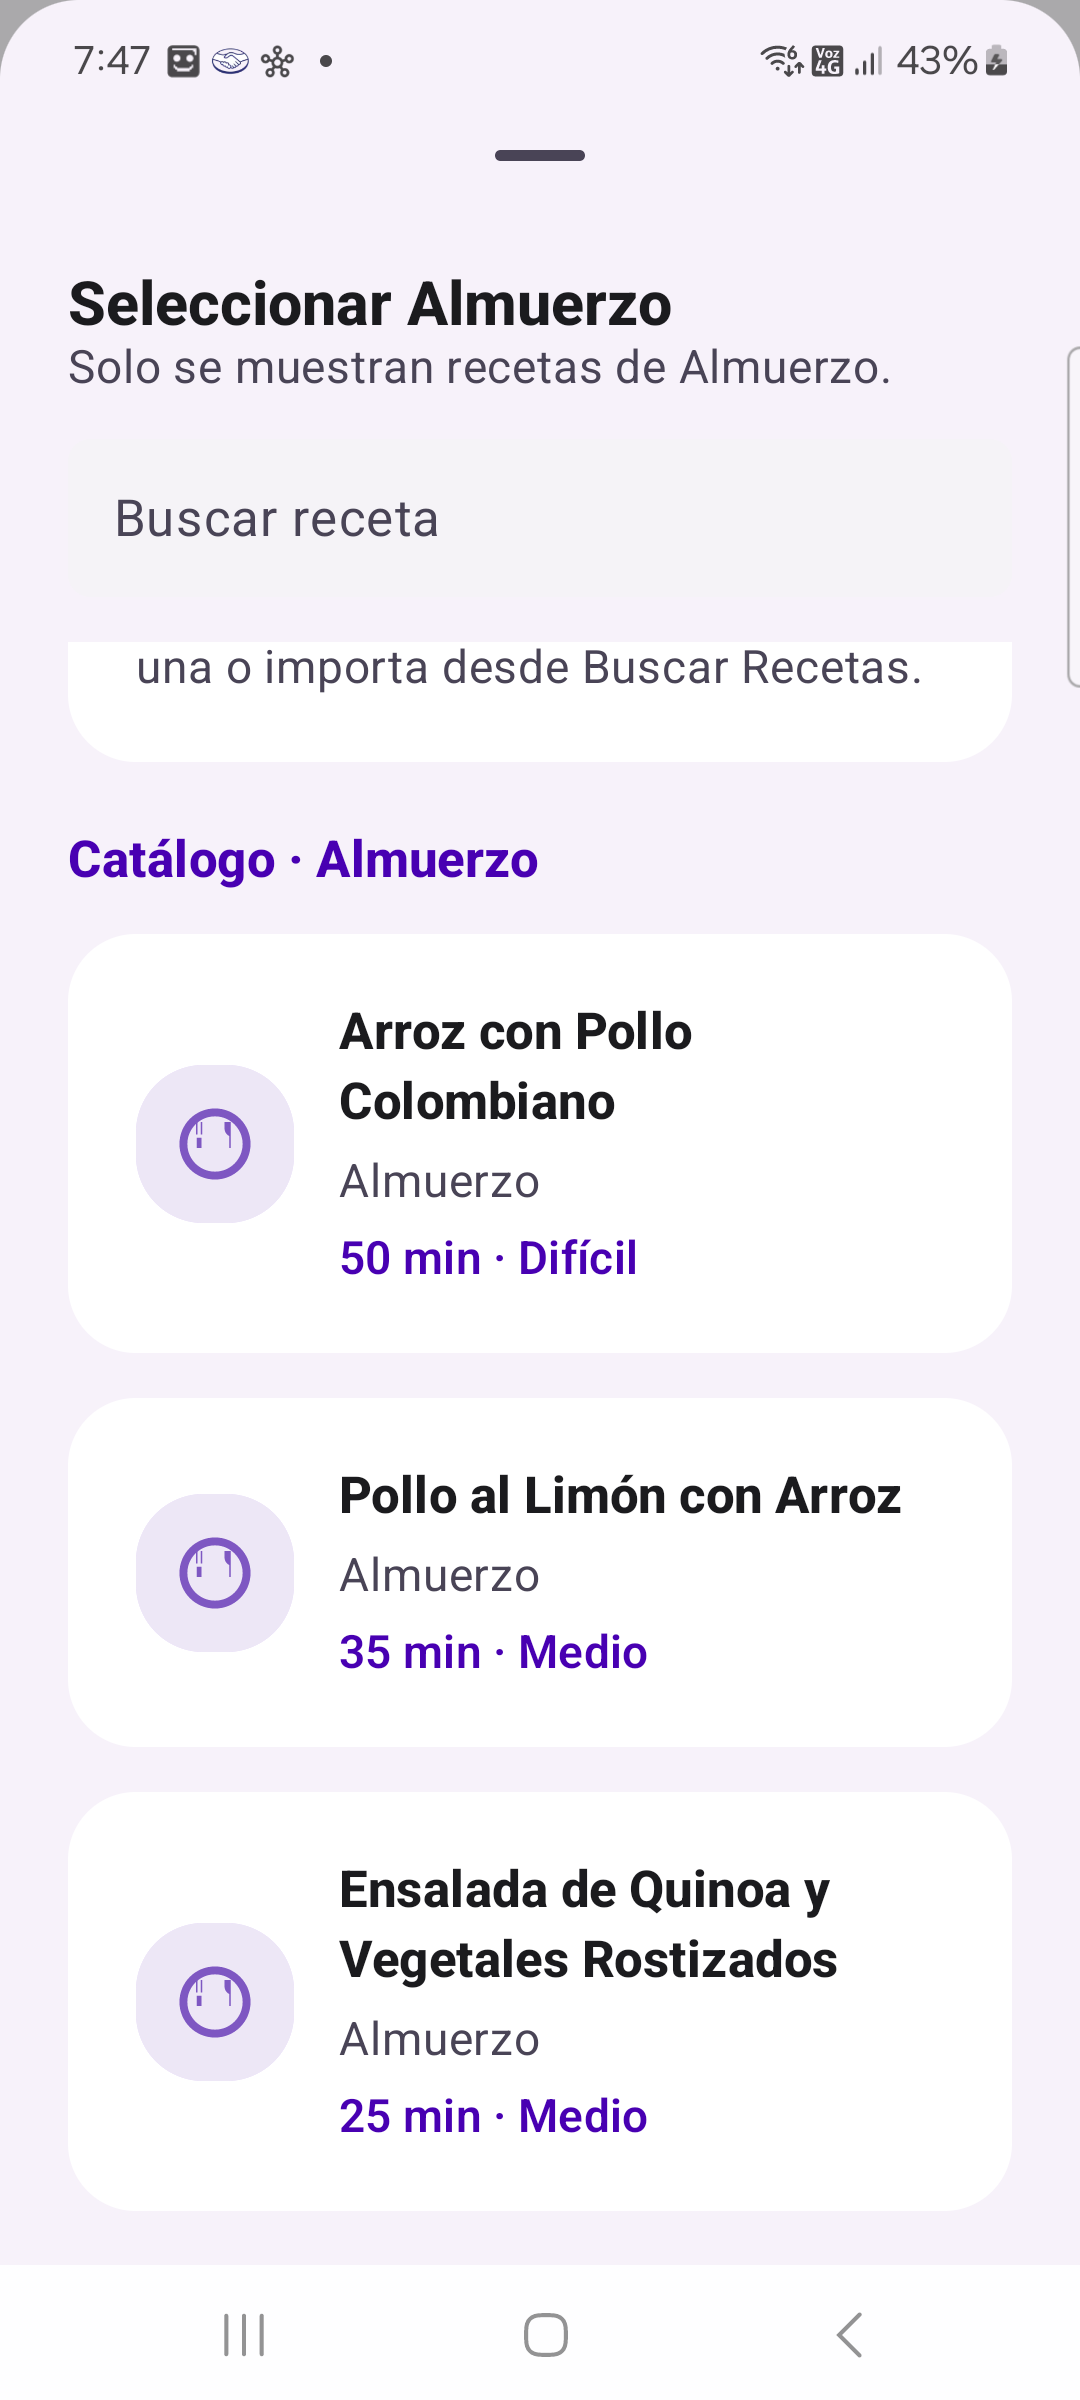
\includegraphics[width=0.30\textwidth]{screenshot_globalsearch.png}
\caption{Captura de pantalla --- GlobalRecipeSearchFragment con campo de búsqueda y
resultados combinados de Room y TheMealDB API. Elaboración propia.}
\label{fig:ss_globalsearch}
\end{figure}

\textbf{LeftMenuFragment (fragment central del requisito del proyecto)}

\noindent\textbf{Archivo:} \texttt{presentation/leftmenu/LeftMenuFragment.kt}

\noindent\textbf{Función:} Este es el fragmento principal exigido por los requisitos del
proyecto. Implementa el layout de dos paneles simultáneos en la misma pantalla:

\begin{itemize}[nosep]
    \item \textbf{Panel izquierdo (25\% del ancho):} \texttt{LeftMenuScreen} --- muestra
    una lista vertical con cinco opciones de navegación: Perfil, Fotos, Video, Web y
    Controles.
    \item \textbf{Panel derecho (75\% del ancho):} el contenido cambia dinámicamente según
    la opción seleccionada en el panel izquierdo.
\end{itemize}

\begin{longtable}{@{}p{2.5cm}p{3.5cm}p{9.5cm}@{}}
\caption{Opciones del panel izquierdo y composables del panel derecho en LeftMenuFragment}
\label{tab:leftmenupaneles}\\
\toprule
\textbf{Opción seleccionada} & \textbf{Composable en panel derecho} &
\textbf{Funcionalidad} \\
\midrule
\endfirsthead
\toprule
\textbf{Opción seleccionada} & \textbf{Composable en panel derecho} &
\textbf{Funcionalidad} \\
\midrule
\endhead
\midrule
\multicolumn{3}{r}{\small\textit{Continúa en la página siguiente}}\\
\endfoot
\bottomrule
\endlastfoot
Perfil & \texttt{ProfileHubScreen} / \texttt{ProfileScreen} & Foto del usuario,
información de estudios y experiencia con scroll vertical \\[3pt]
Fotos & \texttt{PhotosScreen} & Galería de imágenes con \texttt{LazyColumn} (scroll),
muestra descripción al seleccionar una imagen \\[3pt]
Video & \texttt{VideoScreen} & Reproductor de video local con \texttt{VideoView} nativo
+ \texttt{MediaController} (controles de reproducción) \\[3pt]
Web & \texttt{WebScreen} & Navegador web integrado con \texttt{WebView}, campo de texto
para ingresar URL y botón ``IR'' \\[3pt]
Controles & \texttt{ControlsScreen} & Demostración de controles: \texttt{Button},
\texttt{ElevatedButton}, \texttt{IconButton}, \texttt{Checkbox}, \texttt{RadioButton},
\texttt{Switch}, \texttt{Slider} y \texttt{Dropdown} \\
\end{longtable}

La navegación entre paneles se gestiona mediante un estado local
(\texttt{remember \{ mutableStateOf(LeftMenuPanel.Profile) \}}) que al cambiar actualiza
reactivamente el contenido del panel derecho sin necesidad de recargar el fragmento.

\begin{figure}[H]
\centering
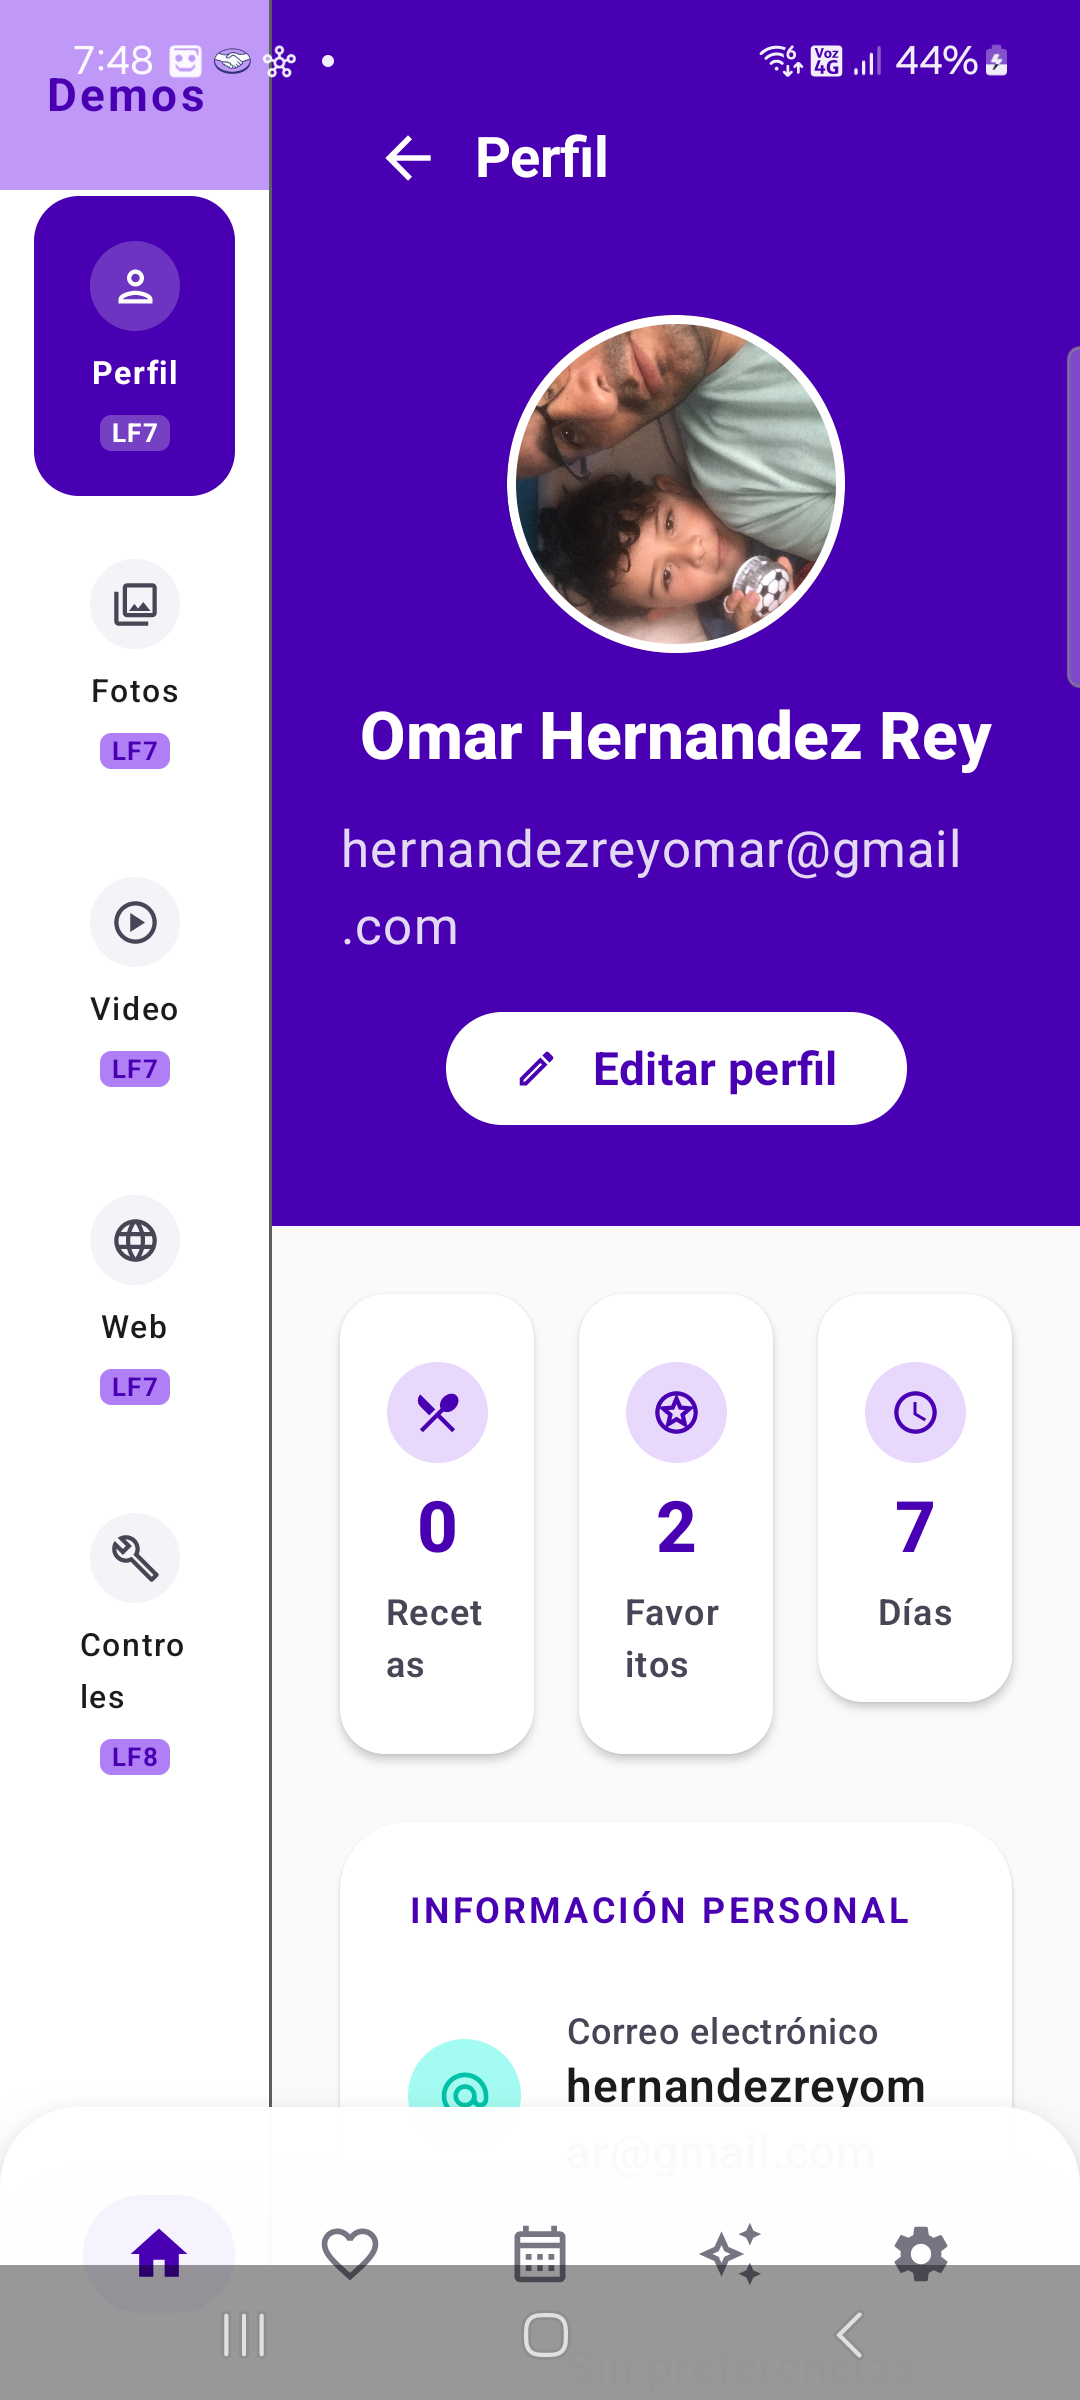
\includegraphics[width=0.30\textwidth]{screenshot_leftmenu_twopanels.png}
\caption{Captura de pantalla --- LeftMenuFragment mostrando el layout de dos paneles
simultáneos: menú izquierdo con opciones y panel derecho con contenido dinámico.
Elaboración propia.}
\label{fig:ss_leftmenu}
\end{figure}

\textbf{Resumen general de componentes}

{\footnotesize
\begin{longtable}{@{}p{4cm}p{4cm}p{2.5cm}p{4.5cm}@{}}
\caption{Resumen de actividades y fragmentos de Recipe Generator}
\label{tab:resumencomponentes}\\
\toprule
\textbf{Componente} & \textbf{Clase} & \textbf{Tipo} & \textbf{Pantalla} \\
\midrule
\endfirsthead
\toprule
\textbf{Componente} & \textbf{Clase} & \textbf{Tipo} & \textbf{Pantalla} \\
\midrule
\endhead
\midrule
\multicolumn{4}{r}{\small\textit{Continúa en la página siguiente}}\\
\endfoot
\bottomrule
\endlastfoot
MainActivity & MainActivity.kt & Activity & Shell principal + Auth \\[3pt]
RecipeDetailActivity & RecipeDetailActivity.kt & Activity & Detalle de receta \\[3pt]
HomeFragment & HomeFragment.kt & Fragment & Menú semanal \\[3pt]
FavoritesFragment & FavoritesFragment.kt & Fragment & Recetas favoritas \\[3pt]
MenuGeneratorFragment & MenuGeneratorFragment.kt & Fragment & Generador con IA \\[3pt]
SettingsFragment & SettingsFragment.kt & Fragment & Configuración \\[3pt]
GlobalRecipeSearchFragment & GlobalRecipeSearchFragment.kt & Fragment & Búsqueda global \\[3pt]
LeftMenuFragment & LeftMenuFragment.kt & Fragment & Layout dos paneles \\[3pt]
ComposeScreenFragment & ComposeScreenFragment.kt & Fragment (abstracto) & Clase base \\
\end{longtable}
}

%+---------------------------------------------------------------+
\subsection{Creación de la interfaz para cada Actividad y/o Fragmento}
\label{sec:creacioninterfaz}

La aplicación utiliza Jetpack Compose como sistema de interfaz gráfica, el estándar
oficial de Android desde 2021. En Compose, las interfaces se construyen mediante
funciones anotadas con \texttt{@Composable} en lugar de archivos XML de layout (a
excepción de \texttt{activity\_main.xml} y \texttt{fragment\_global\_recipe\_search.xml},
que mantienen el esquema XML tradicional). Cada pantalla se construye como una jerarquía
de composables que declaran de forma reactiva los elementos visuales.

A continuación se describe la interfaz creada para cada Actividad y Fragmento de la
aplicación.

\subsubsection{MainActivity --- Interfaz raíz}

\noindent\textbf{Archivo de layout:} \texttt{res/layout/activity\_main.xml}

La interfaz de \texttt{MainActivity} está definida en el único archivo XML de layout de
la aplicación. Contiene un único elemento: un \texttt{FragmentContainerView} que ocupa
toda la pantalla y sirve como contenedor del sistema de navegación.

\begin{lstlisting}[language=XML, caption={Layout XML de activity\_main.xml}]
<?xml version="1.0" encoding="utf-8"?>
<androidx.fragment.app.FragmentContainerView
    xmlns:android="http://schemas.android.com/apk/res/android"
    xmlns:app="http://schemas.android.com/apk/res-auto"
    android:id="@+id/nav_host_fragment"
    android:layout_width="match_parent"
    android:layout_height="match_parent"
    app:defaultNavHost="true"
    app:navGraph="@navigation/main_nav_graph" />
\end{lstlisting}

Por encima de este contenedor, \texttt{MainActivity} inyecta su contenido Compose
mediante \texttt{setContent \{\}}, que muestra según el estado de autenticación uno de
los composables descritos en la tabla~\ref{tab:mainactivityestados}.

\begin{table}[H]
\caption{Estados de autenticación y composables mostrados en MainActivity}
\label{tab:mainactivityestados}
\begin{tabularx}{\textwidth}{@{}lX@{}}
\toprule
\textbf{Estado} & \textbf{Composable mostrado} \\
\midrule
Verificando auth & \texttt{LoadingBox} --- \texttt{CircularProgressIndicator} centrado \\[3pt]
Sin sesión & \texttt{AuthScreen} --- pantalla de login/registro \\[3pt]
Login nuevo & \texttt{AuthWelcomeScreen} --- bienvenida al usuario \\[3pt]
Sesión activa & \texttt{AppShell} --- shell completo con navegación inferior \\
\bottomrule
\end{tabularx}
\end{table}

\subsubsection{RecipeDetailActivity --- Detalle de receta}

\noindent\textbf{Tipo:} Compose puro (\texttt{setContent \{\}})

La interfaz se compone de los siguientes elementos visuales apilados verticalmente:
\texttt{TopAppBar} con botón de retroceso (\texttt{IconButton} $\leftarrow$
\texttt{ArrowBack}), imagen de la receta con \texttt{ContentScale.Crop} en relación de
aspecto 16:9, título con estilo \texttt{headlineMedium}, chips de metadata (categoría,
tiempo, calorías, dificultad), botón de favorito con \texttt{animateColorAsState}
(corazón rojo/gris), sección de ingredientes en \texttt{LazyColumn}, lista numerada de
pasos de preparación, y botón de video que abre YouTube en el navegador. Todo el
contenido principal está dentro de un \texttt{Column} con \texttt{verticalScroll}.

\begin{figure}[H]
\centering
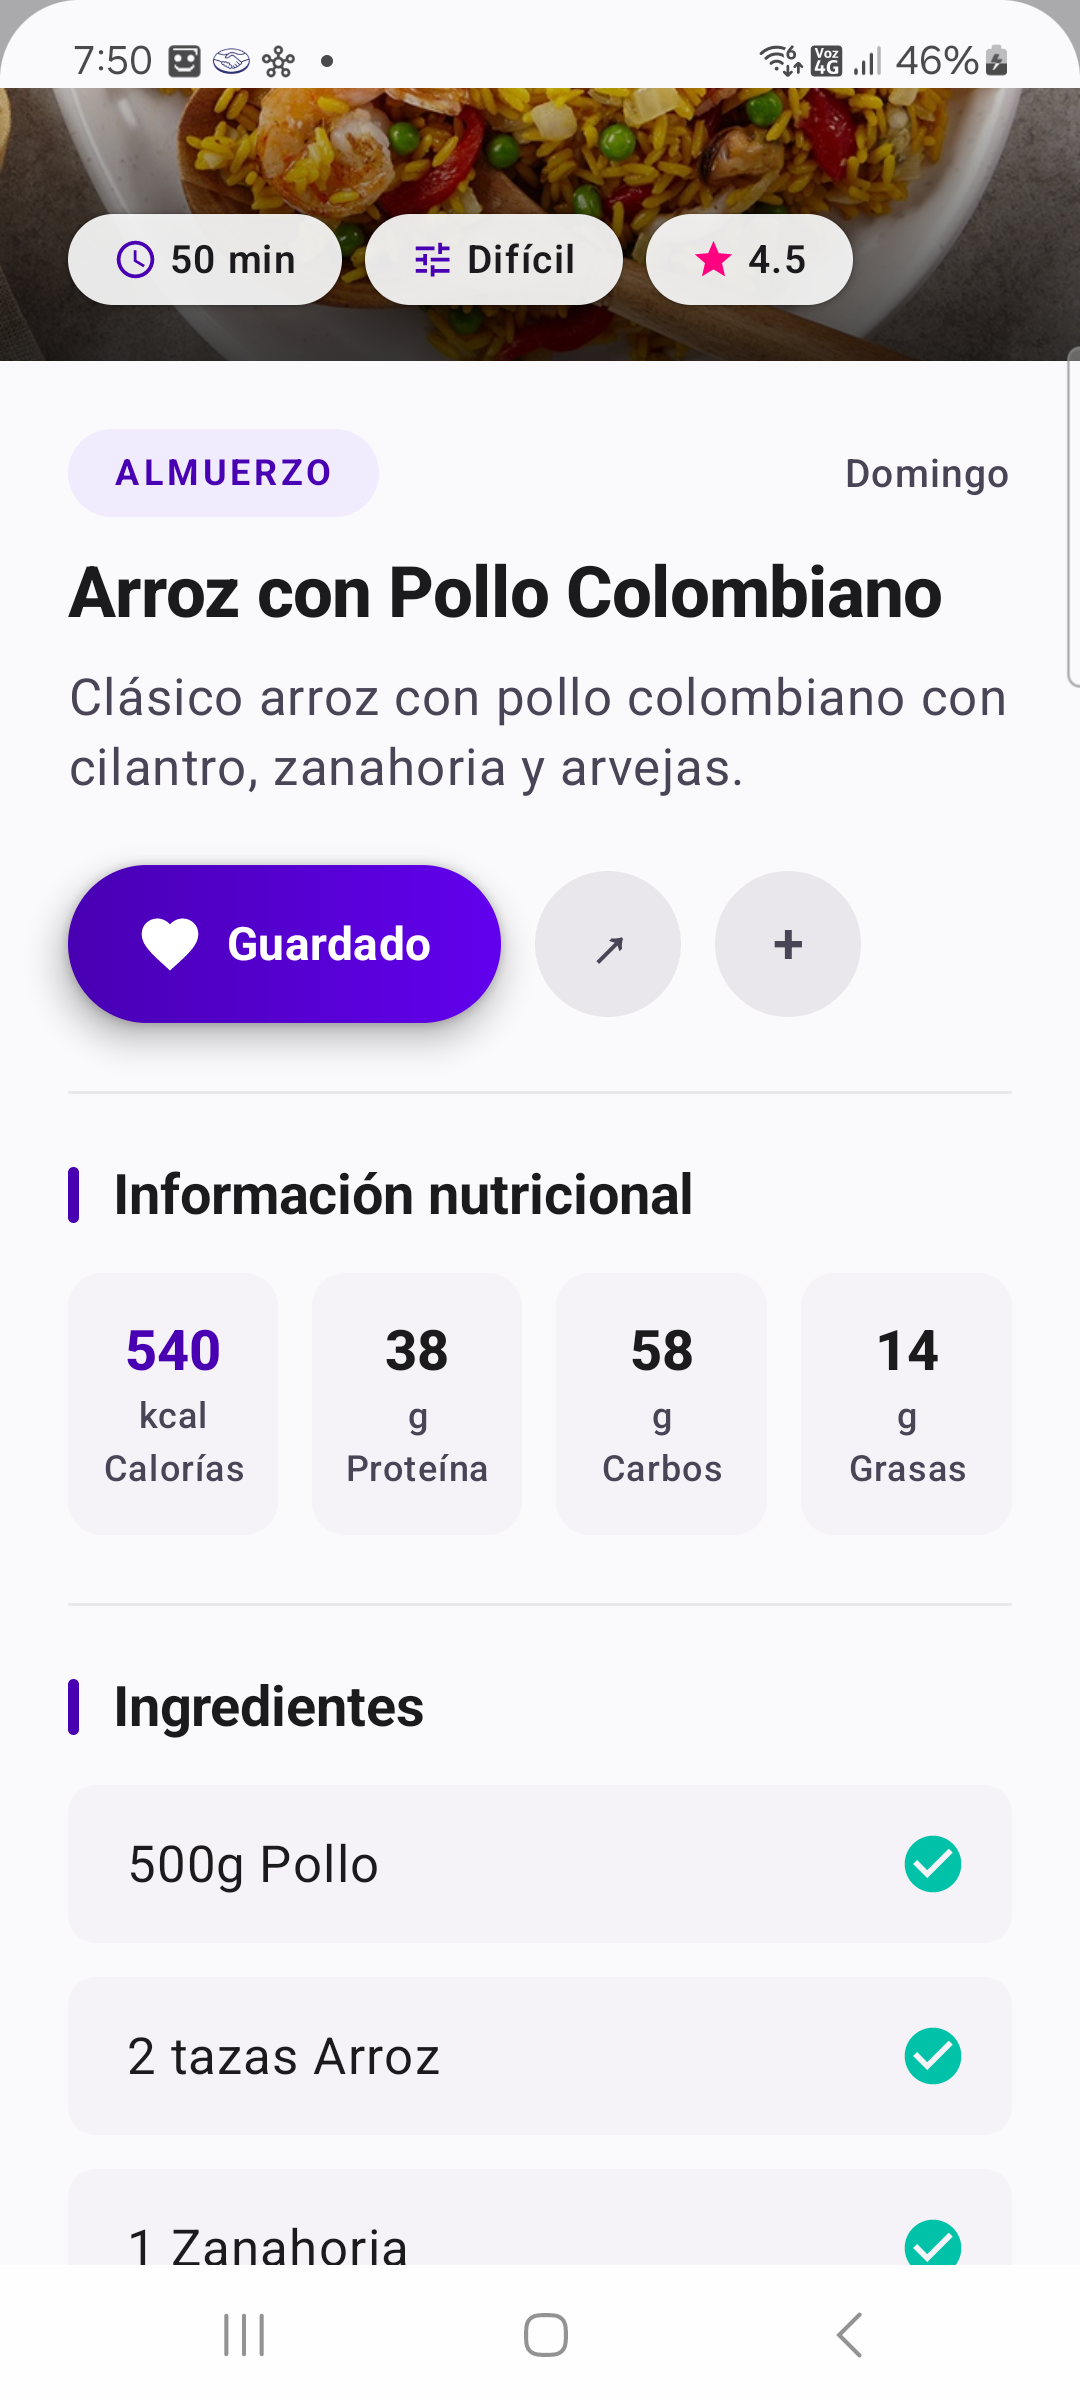
\includegraphics[width=0.30\textwidth]{screenshot_recipedetail_interfaz.png}
\caption{Interfaz de RecipeDetailActivity --- composables apilados verticalmente con
imagen, metadata, ingredientes y pasos. Elaboración propia.}
\label{fig:ss_recipedetail_ui}
\end{figure}

\subsubsection{ComposeScreenFragment --- Fragmento base abstracto}

\noindent\textbf{Tipo:} Crea un \texttt{ComposeView} programáticamente en
\texttt{onCreateView()}.

No tiene interfaz propia. Su función es crear el contenedor Compose
(\texttt{ComposeView}) que sirve como host para el contenido visual definido en la
subclase concreta. Aplica el \texttt{RecipeGeneratorTheme} con el tema claro/oscuro del
usuario antes de delegar al método \texttt{ScreenContent()}.

\subsubsection{HomeFragment $\rightarrow$ RecipeListScreen --- Menú semanal}

\noindent\textbf{Tipo:} Compose vía \texttt{ComposeScreenFragment}.

Interfaz construida con los siguientes elementos: \texttt{TopAppBar} personalizado con
título ``RecipeGenerator'' e ícono de perfil, pestañas de días en
\texttt{ScrollableTabRow} con los 7 días de la semana (el día activo se resalta), lista
de recetas del día en \texttt{LazyColumn} donde cada ítem es una \texttt{Card} con
imagen, nombre, metadata y botón de favorito, barra de navegación inferior
(\texttt{NavigationBar}) con 4 ítems (Inicio, Favoritos, Generador, Ajustes), e
indicador de sincronización (\texttt{LinearProgressIndicator}) visible durante sync con
Firestore.

\begin{figure}[H]
\centering
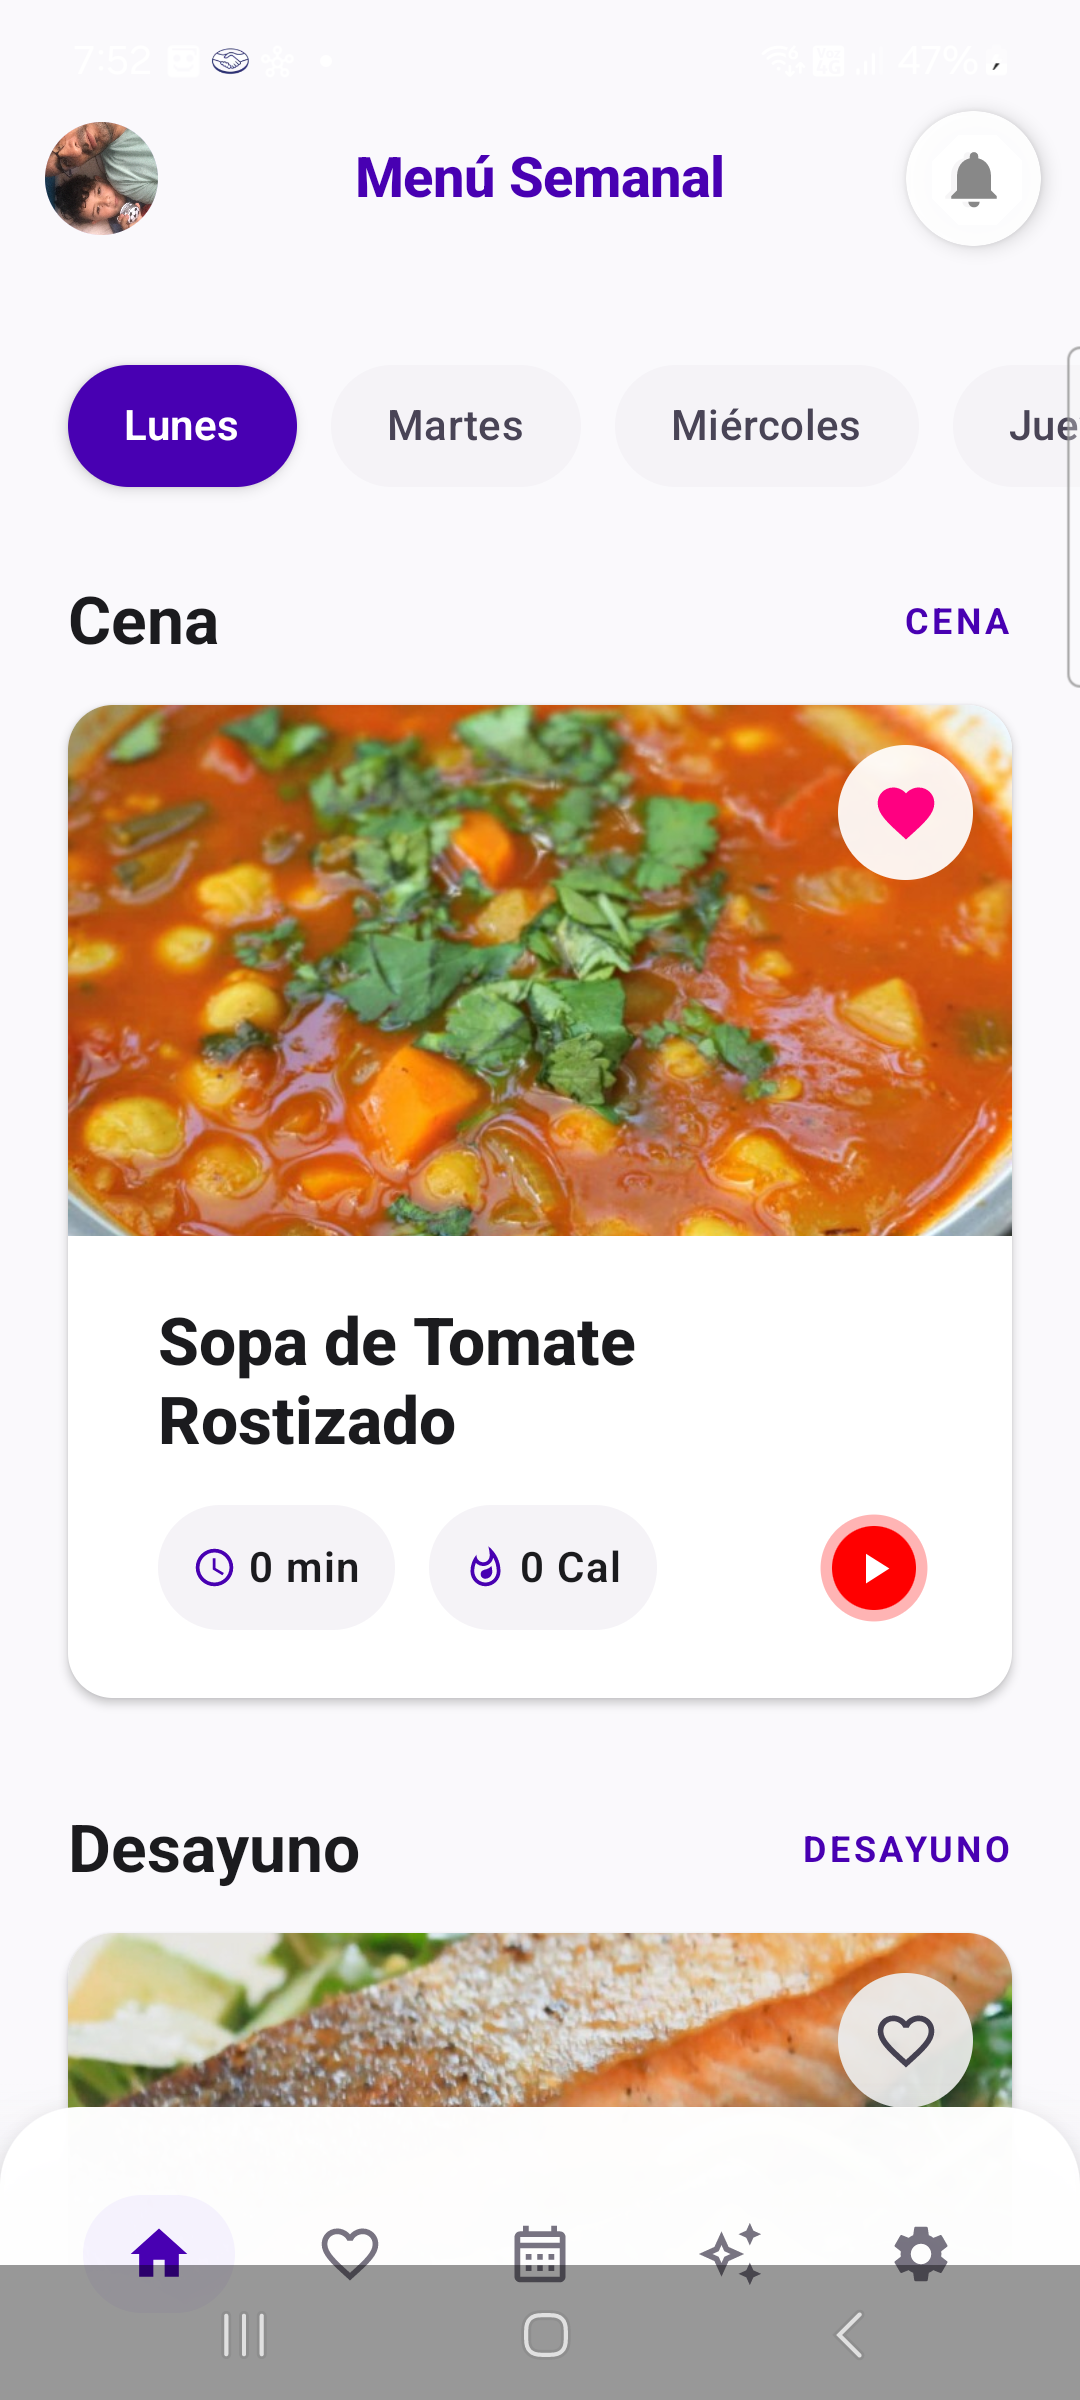
\includegraphics[width=0.30\textwidth]{screenshot_home_interfaz.png}
\caption{Interfaz de HomeFragment --- TopAppBar, pestañas de días, lista de recetas y
barra de navegación inferior. Elaboración propia.}
\label{fig:ss_home_ui}
\end{figure}

\subsubsection{FavoritesFragment $\rightarrow$ FavoritesScreen --- Recetas favoritas}

\noindent\textbf{Tipo:} Compose vía \texttt{ComposeScreenFragment}.

Interfaz con \texttt{TopAppBar} con título ``Favoritos'', campo de búsqueda
(\texttt{OutlinedTextField} con ícono de lupa), filtros de categoría en
\texttt{LazyRow} horizontal con \texttt{FilterChip} para cada categoría (Todos,
Desayuno, Almuerzo, etc.), lista de favoritos en \texttt{LazyColumn} con tarjetas de
receta que incluyen botón de eliminar favorito, estado vacío con ícono y mensaje
cuando no hay resultados, y barra de navegación inferior.

\subsubsection{MenuGeneratorFragment $\rightarrow$ MenuGeneratorScreen --- Generador con IA}

\noindent\textbf{Tipo:} Compose vía \texttt{ComposeScreenFragment}.

Interfaz de configuración del generador con \texttt{TopAppBar} con título ``Generador
de Menús'', sección de dietas mediante grupo de \texttt{FilterChip} para selección
múltiple, selector de dificultad con \texttt{SingleChoiceSegmentedButtonRow} (Fácil /
Medio / Difícil), control de porciones con \texttt{Row} de botones + y $-$ y
\texttt{Text} central, tipos de receta con grupo de \texttt{FilterChip}, botón
``GENERAR MENÚ'' de ancho completo que dispara la llamada a Gemini AI, y modal de
resultado con \texttt{BottomSheetDialog} Compose.

\subsubsection{SettingsFragment $\rightarrow$ SettingsScreen --- Configuración}

\noindent\textbf{Tipo:} Compose vía \texttt{ComposeScreenFragment}.

Interfaz organizada en secciones tipo lista de preferencias: \texttt{TopAppBar} con
título ``Ajustes'', sección Tema con dos \texttt{Card} seleccionables (``Claro'' y
``Oscuro'' con ícono de sol/luna), sección Dietas predeterminadas con grupo de
\texttt{FilterChip}, sección Porciones con botones +/$-$ + número, sección Idioma con
opciones ``Español'' / ``English'' en \texttt{Card} seleccionables, y botón Cerrar
sesión (\texttt{TextButton} en rojo con ícono \texttt{Logout}).

\subsubsection{GlobalRecipeSearchFragment $\rightarrow$ GlobalRecipeSearchScreen --- Búsqueda global}

\noindent\textbf{Archivo de layout:} \texttt{res/layout/fragment\_global\_recipe\_search.xml}

Este fragmento es el único (además de \texttt{MainActivity}) que usa un layout XML
tradicional, que luego embebe un \texttt{ComposeView}:

\begin{lstlisting}[language=XML, caption={Layout XML de fragment\_global\_recipe\_search.xml}]
<?xml version="1.0" encoding="utf-8"?>
<androidx.compose.ui.platform.ComposeView
    xmlns:android="http://schemas.android.com/apk/res/android"
    android:id="@+id/globalRecipeSearchComposeView"
    android:layout_width="match_parent"
    android:layout_height="match_parent" />
\end{lstlisting}

El composable \texttt{GlobalRecipeSearchScreen} cargado dentro contiene:
\texttt{TopAppBar} con botón de retroceso y título ``Buscar recetas'', campo de búsqueda
con \texttt{OutlinedTextField} y animación de activación, indicador de carga
(\texttt{CircularProgressIndicator}) durante la búsqueda, lista de resultados en
\texttt{LazyColumn} con tarjetas que muestran imagen, nombre, origen y categoría de cada
receta, y estado vacío/error con mensaje ilustrado.

\subsubsection{LeftMenuFragment $\rightarrow$ MainScreen + LeftMenuScreen --- Sistema de dos paneles}

\noindent\textbf{Tipo:} Compose vía \texttt{ComposeScreenFragment}.

Este fragmento implementa el requisito principal de la entrega: dos fragmentos en la
misma pantalla, uno a la izquierda y otro a la derecha. La interfaz de
\texttt{MainScreen} se construye con un \texttt{Row} que ocupa toda la pantalla y divide
el espacio en dos paneles.

\begin{figure}[H]
\centering
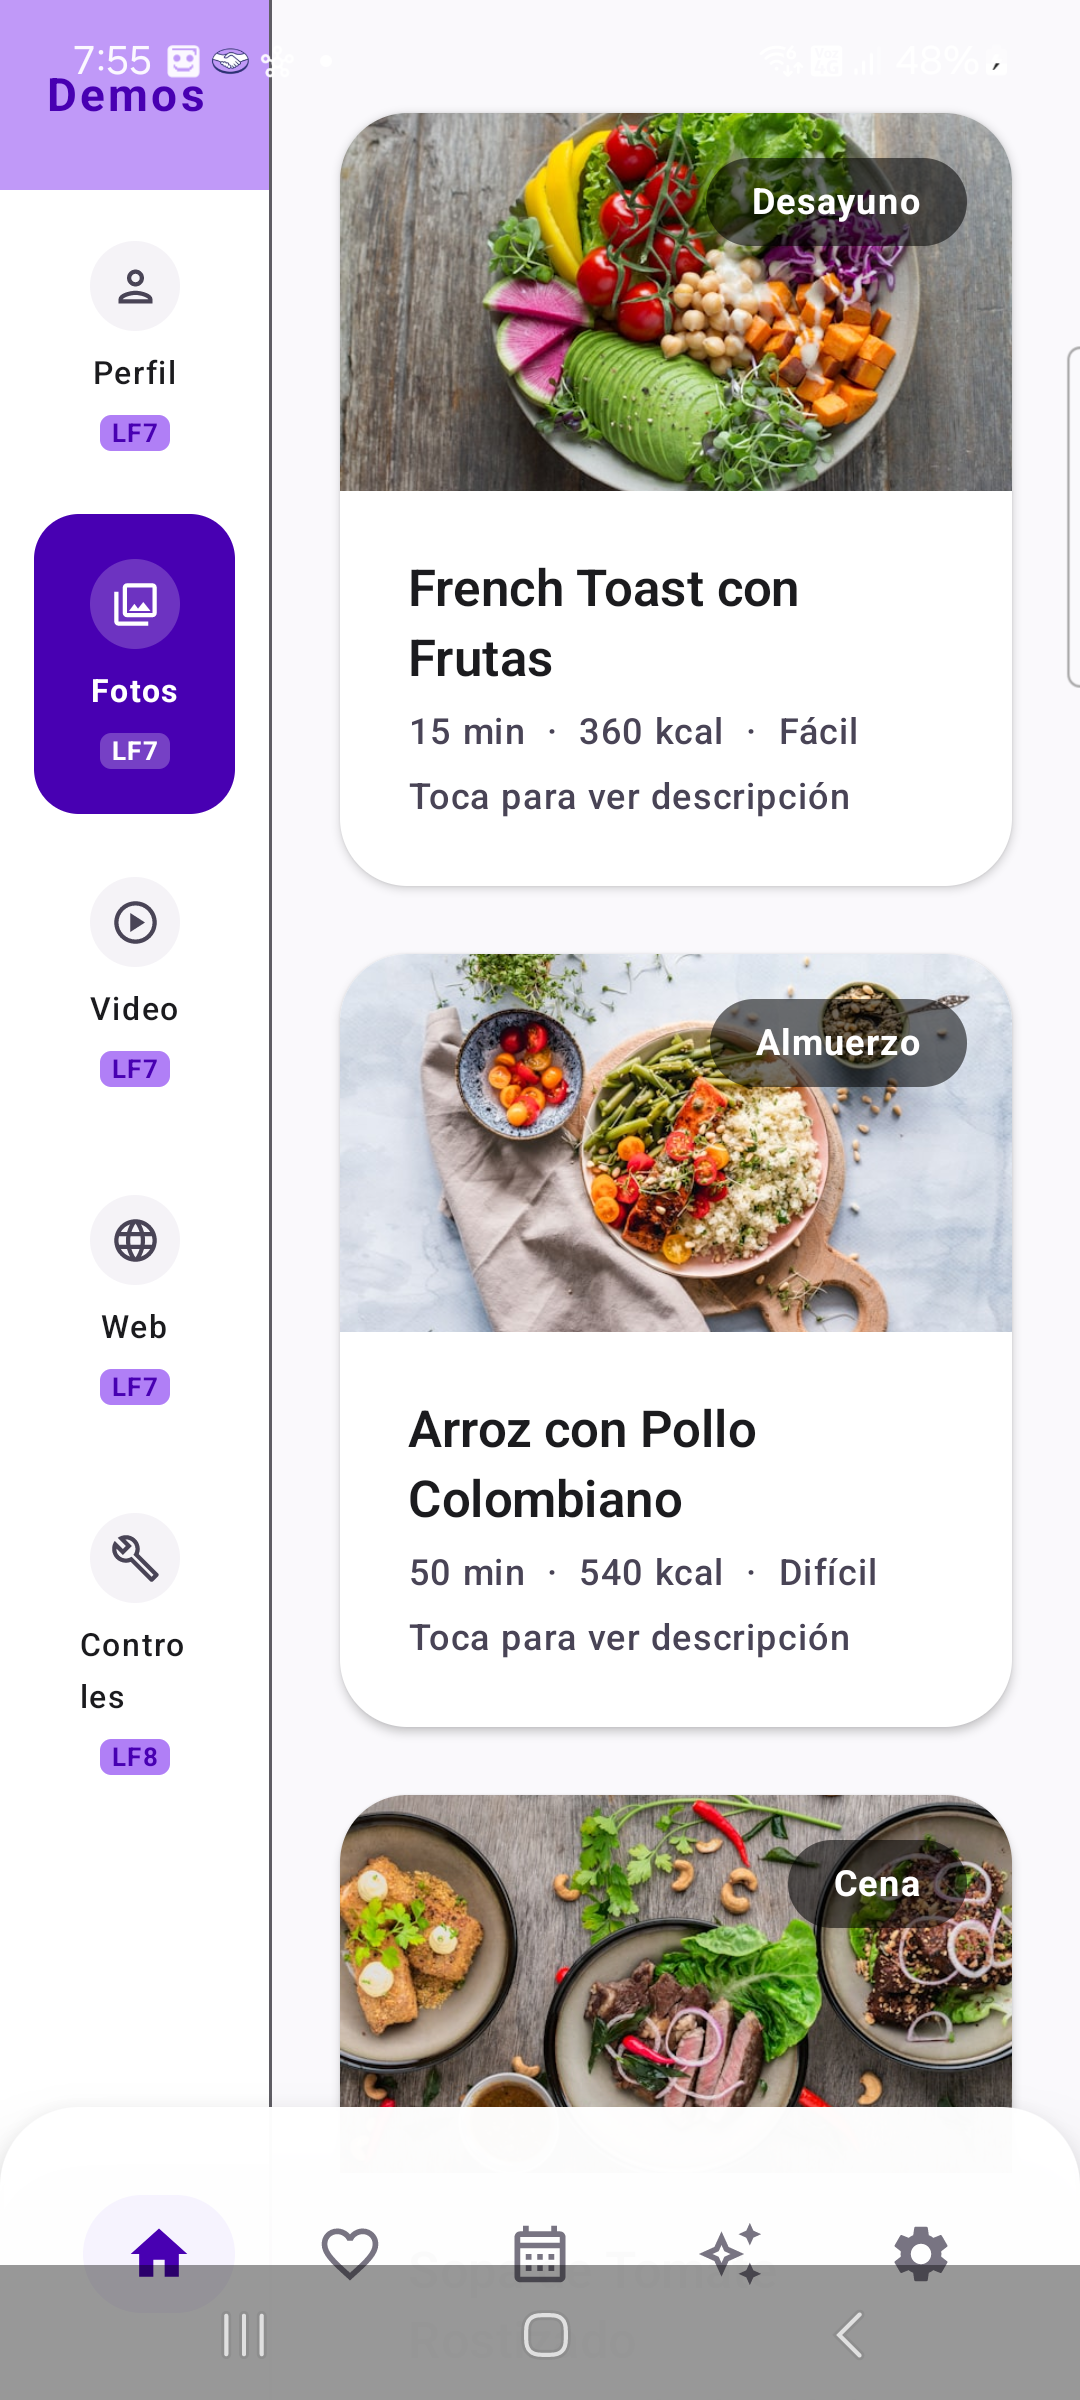
\includegraphics[width=0.30\textwidth]{screenshot_leftmenu_layout.png}
\caption{Estructura del layout de dos paneles --- Panel izquierdo (25\%) con menú de
opciones y panel derecho (75\%) con contenido dinámico. Elaboración propia.}
\label{fig:ss_leftmenu_layout}
\end{figure}

\noindent\textbf{Panel izquierdo --- LeftMenuScreen.} Ocupa el 25\% del ancho de la
pantalla. Construido con \texttt{Column} con fondo
\texttt{SurfaceContainerLowest}, encabezado con fondo \texttt{PrimaryContainer} y texto
``Demos'', y lista de opciones en \texttt{LazyColumn} con 5 ítems; cada ítem
(\texttt{LeftMenuItemRow}) contiene un \texttt{Box} circular con \texttt{Icon},
\texttt{Text} con la etiqueta de la opción, badge identificador de categoría, y fondo
animado con \texttt{animateColorAsState} (color primario si está seleccionado,
transparente si no).

\noindent\textbf{Panel derecho --- contenido dinámico.} Ocupa el 75\% del ancho. Muestra
uno de cinco composables según la opción activa:

\textbf{Panel derecho $\rightarrow$ Perfil (ProfileScreen)}

Cabecera con fondo primario que contiene imagen circular (120 dp) con foto de perfil o
iniciales del nombre, nombre completo y correo del usuario, y botón ``Editar perfil''.
Tarjetas de estadísticas en \texttt{Row} con 3 \texttt{StatCard}: Recetas creadas,
Favoritos, Días planificados. Sección INFORMACIÓN PERSONAL con \texttt{Card} con filas
ícono + etiqueta + valor. Sección ESTUDIOS con \texttt{Card} con caja de altura fija
(140 dp) y \texttt{verticalScroll} propio. Sección EXPERIENCIA con idéntica estructura.
Acciones rápidas con dos \texttt{Card} clicables: ``Mis recetas'' y ``Plan semanal''.
Botón cerrar sesión (\texttt{TextButton} en rojo al fondo). Todo dentro de
\texttt{Column} con \texttt{verticalScroll} global.

\begin{figure}[H]
\centering
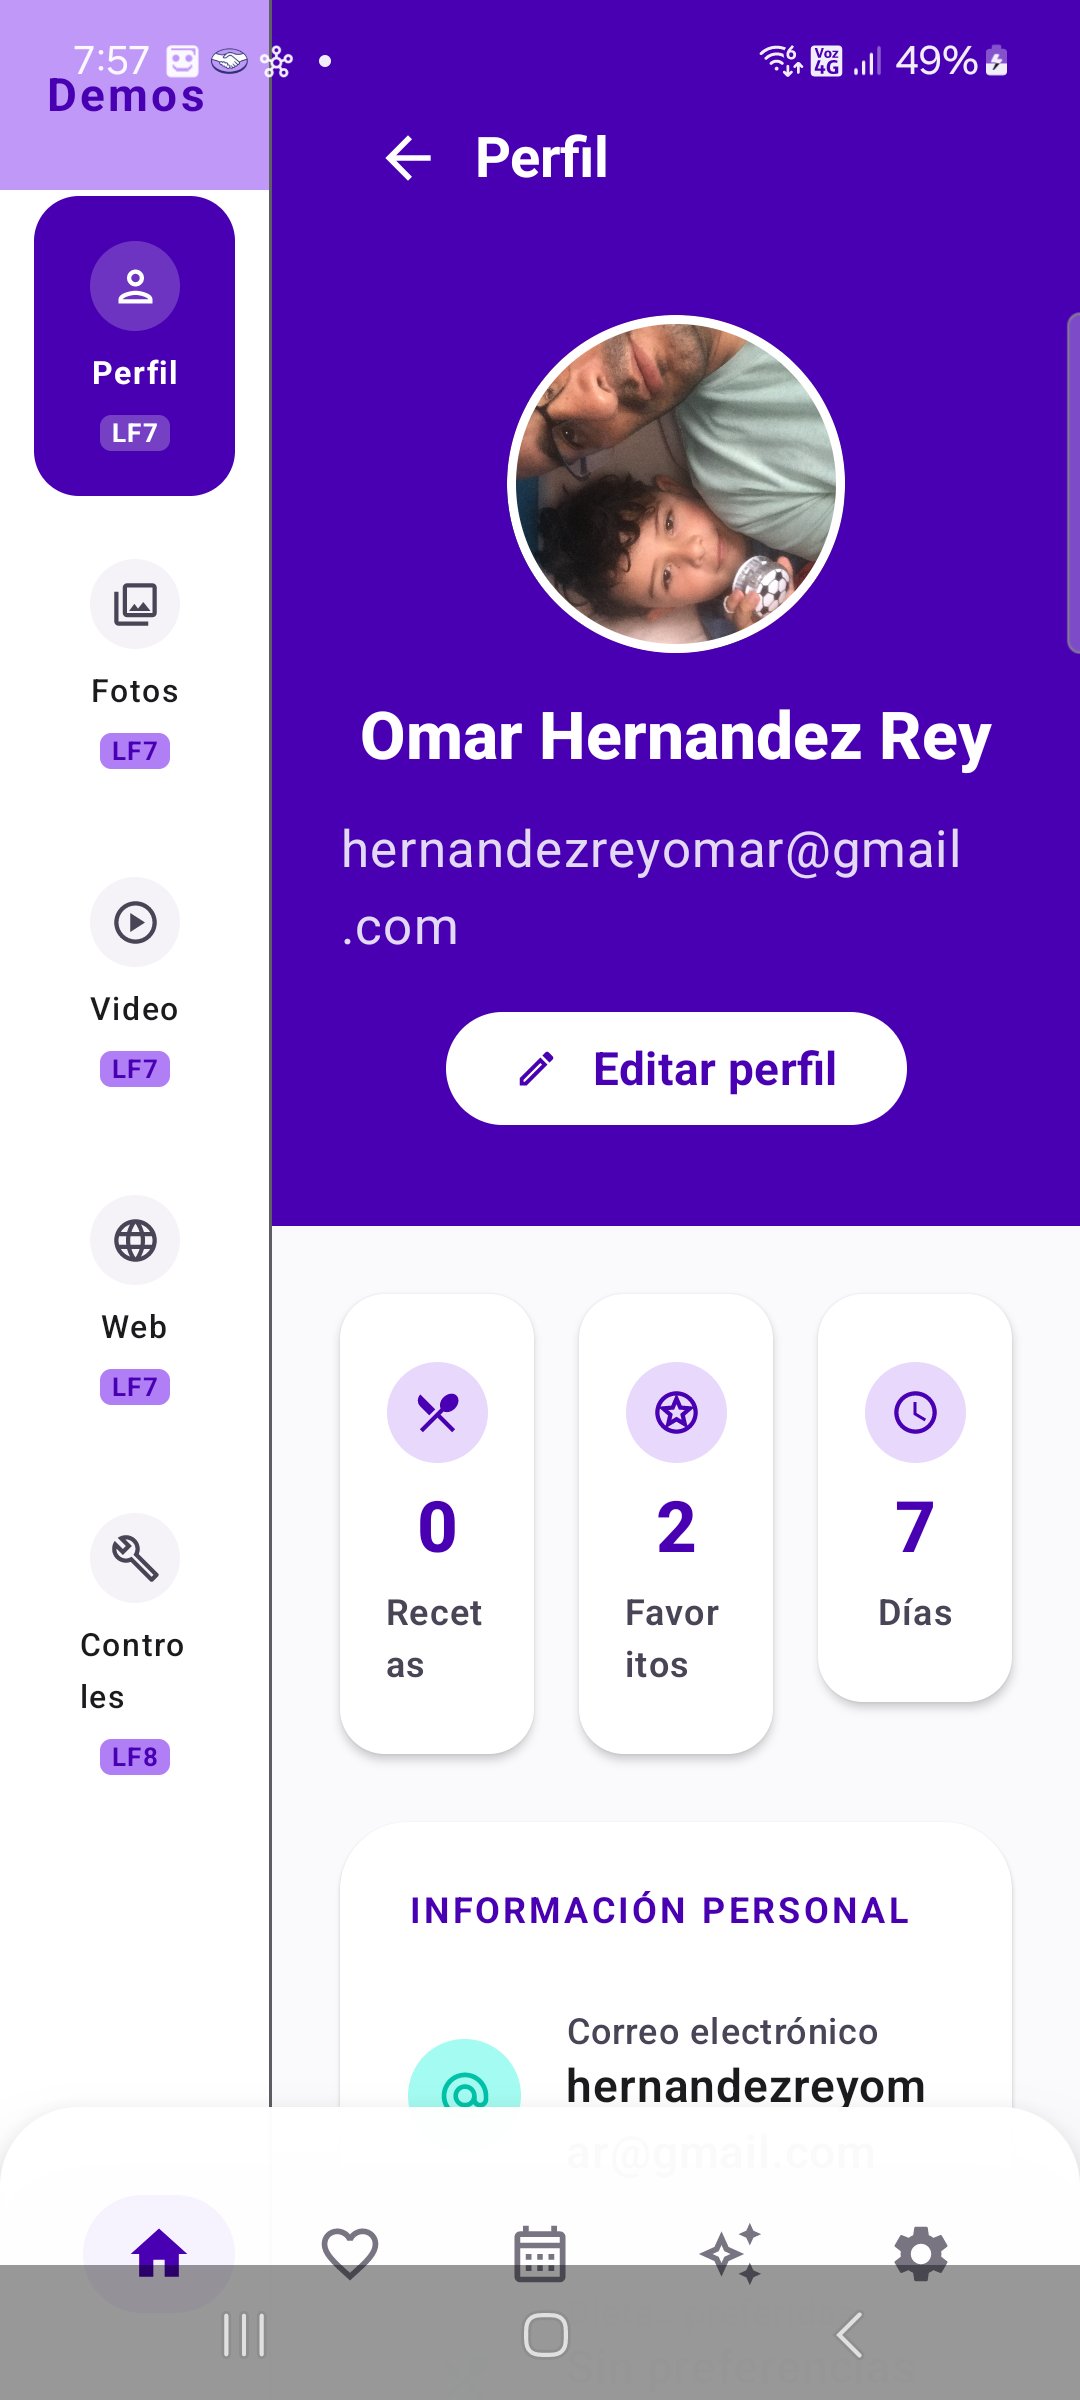
\includegraphics[width=0.30\textwidth]{screenshot_profile.png}
\caption{Panel derecho Perfil --- cabecera con foto, estadísticas, información personal,
estudios y experiencia con scroll. Elaboración propia.}
\label{fig:ss_profile}
\end{figure}

\textbf{Panel derecho $\rightarrow$ Fotos (PhotosScreen)}

Panel de descripción que aparece/desaparece con \texttt{animateColorAsState} al
seleccionar una imagen, mostrando título, descripción, dificultad y día de la receta.
Galería en \texttt{LazyColumn} con tarjetas \texttt{RecipePhotoCard}: cada tarjeta tiene
imagen 16:9, badge de categoría, badge ``Seleccionada'' cuando está activa, nombre,
tiempo, calorías y texto de interacción al pie.

\begin{figure}[H]
\centering
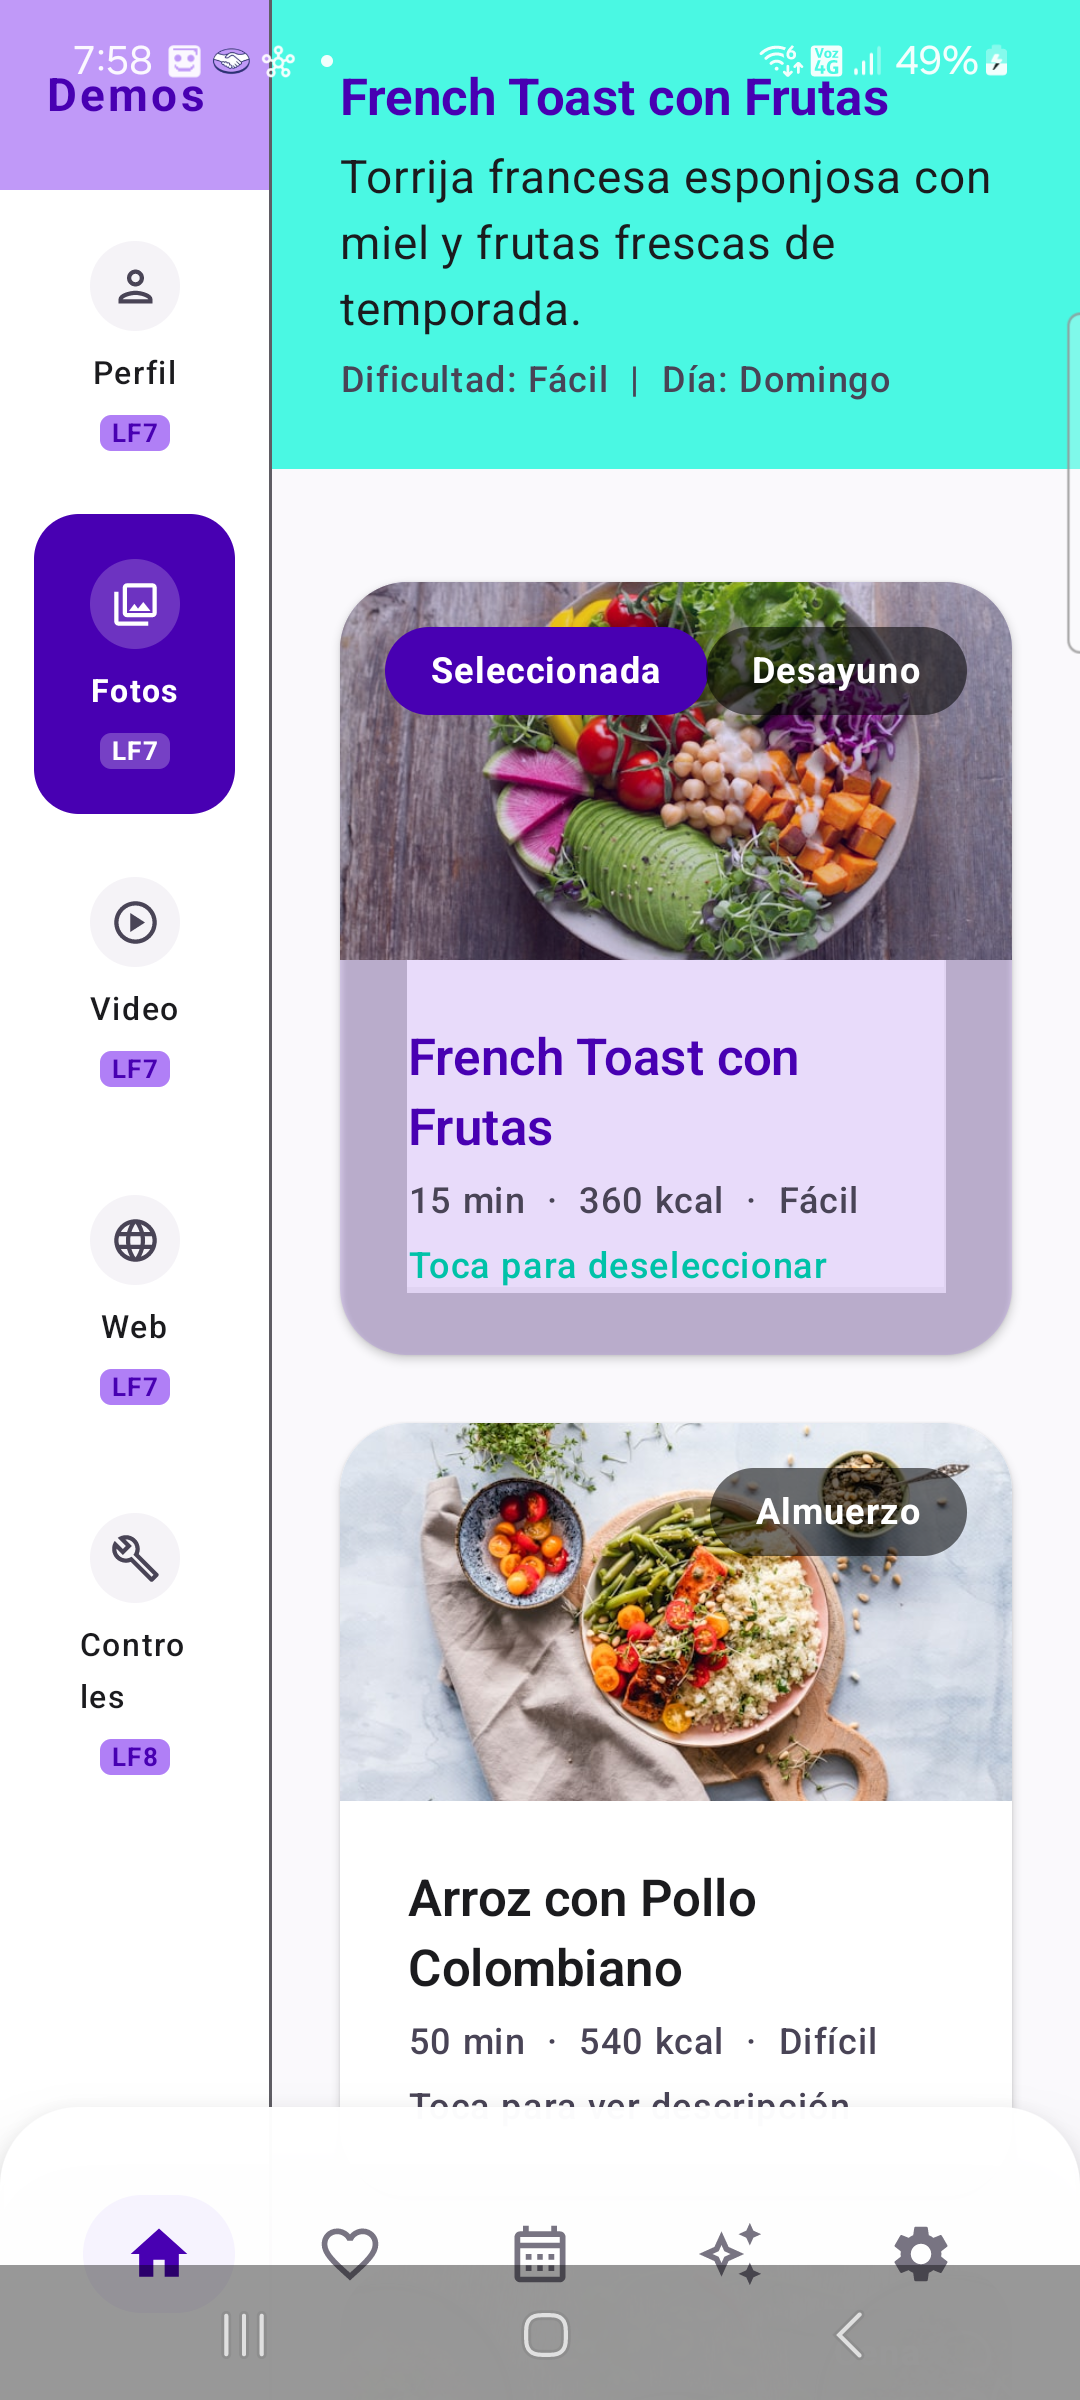
\includegraphics[width=0.30\textwidth]{screenshot_photos.png}
\caption{Panel derecho Fotos --- galería de imágenes con selección y panel de descripción
dinámico. Elaboración propia.}
\label{fig:ss_photos}
\end{figure}

\textbf{Panel derecho $\rightarrow$ Video (VideoScreen)}

\texttt{Column} con \texttt{verticalScroll} que contiene título ``Tutoriales de cocina'',
texto descriptivo, \texttt{Card} con fondo negro que aloja un
\texttt{AndroidView \{ VideoView \}} en relación 16:9 con \texttt{MediaController}
nativo (barra de play/pausa/progreso/volumen),
\texttt{CircularProgressIndicator} mientras carga, pantalla de error/fallback si el
video no carga, y \texttt{Card} ``ACERCA DEL VIDEO'' con descripción del contenido.

\begin{figure}[H]
\centering
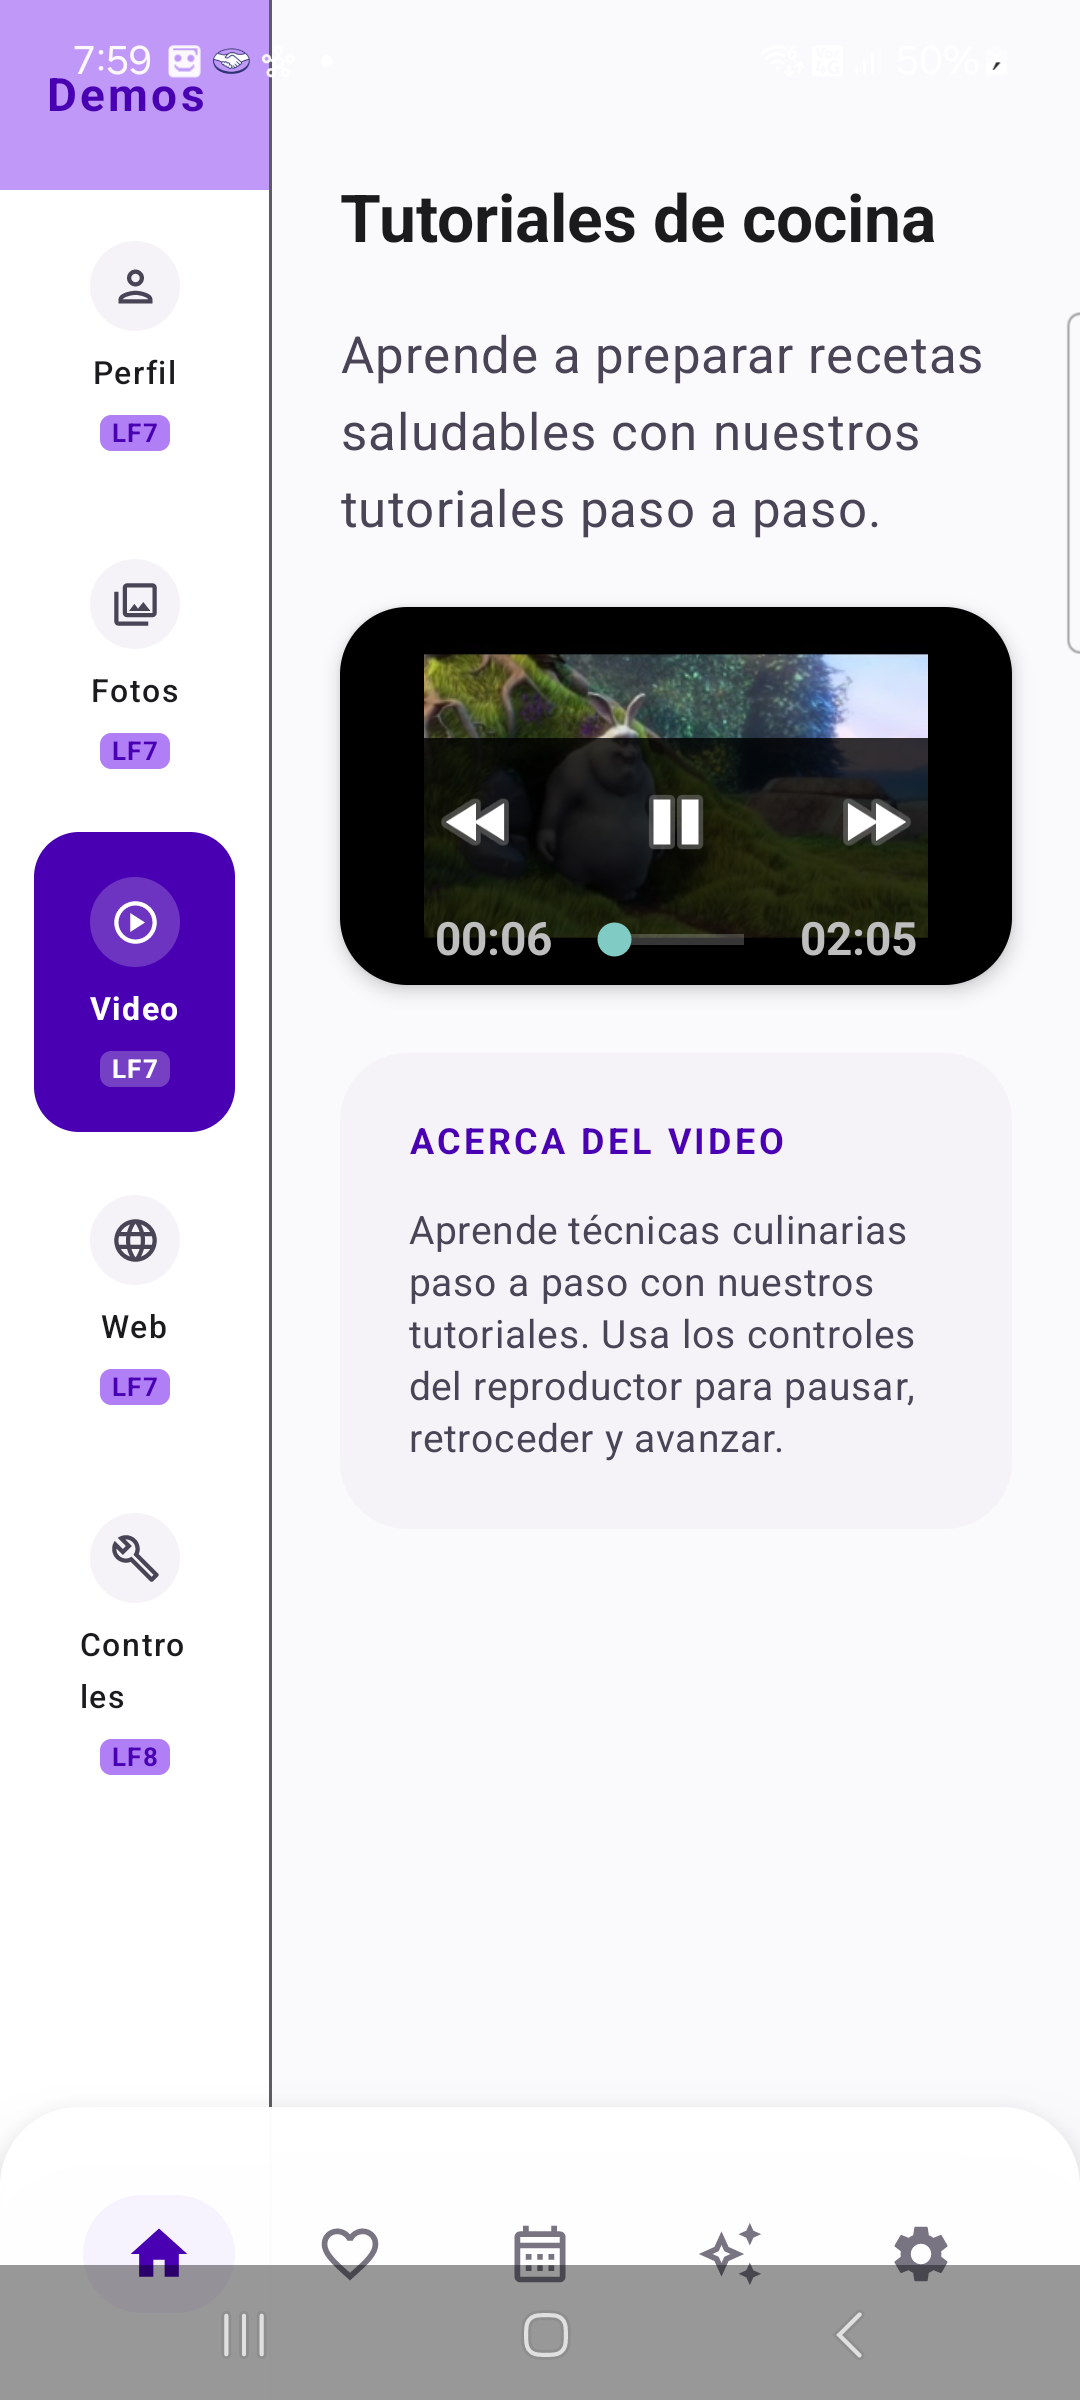
\includegraphics[width=0.30\textwidth]{screenshot_video.png}
\caption{Panel derecho Video --- reproductor con VideoView nativo y controles
MediaController integrados. Elaboración propia.}
\label{fig:ss_video}
\end{figure}

\textbf{Panel derecho $\rightarrow$ Web (WebScreen)}

\texttt{Column} sin scroll (el scroll lo hace el \texttt{WebView}): barra de navegación
con \texttt{OutlinedTextField} con ícono de globo terráqueo, placeholder ``Ingresa una
URL...'' e ícono de recarga (\texttt{IconButton}), botón ``IR'' alineado a la derecha,
\texttt{LinearProgressIndicator} visible durante la carga de página, y
\texttt{AndroidView \{ WebView \}} con peso 1f (ocupa el resto de la pantalla).

\begin{figure}[H]
\centering
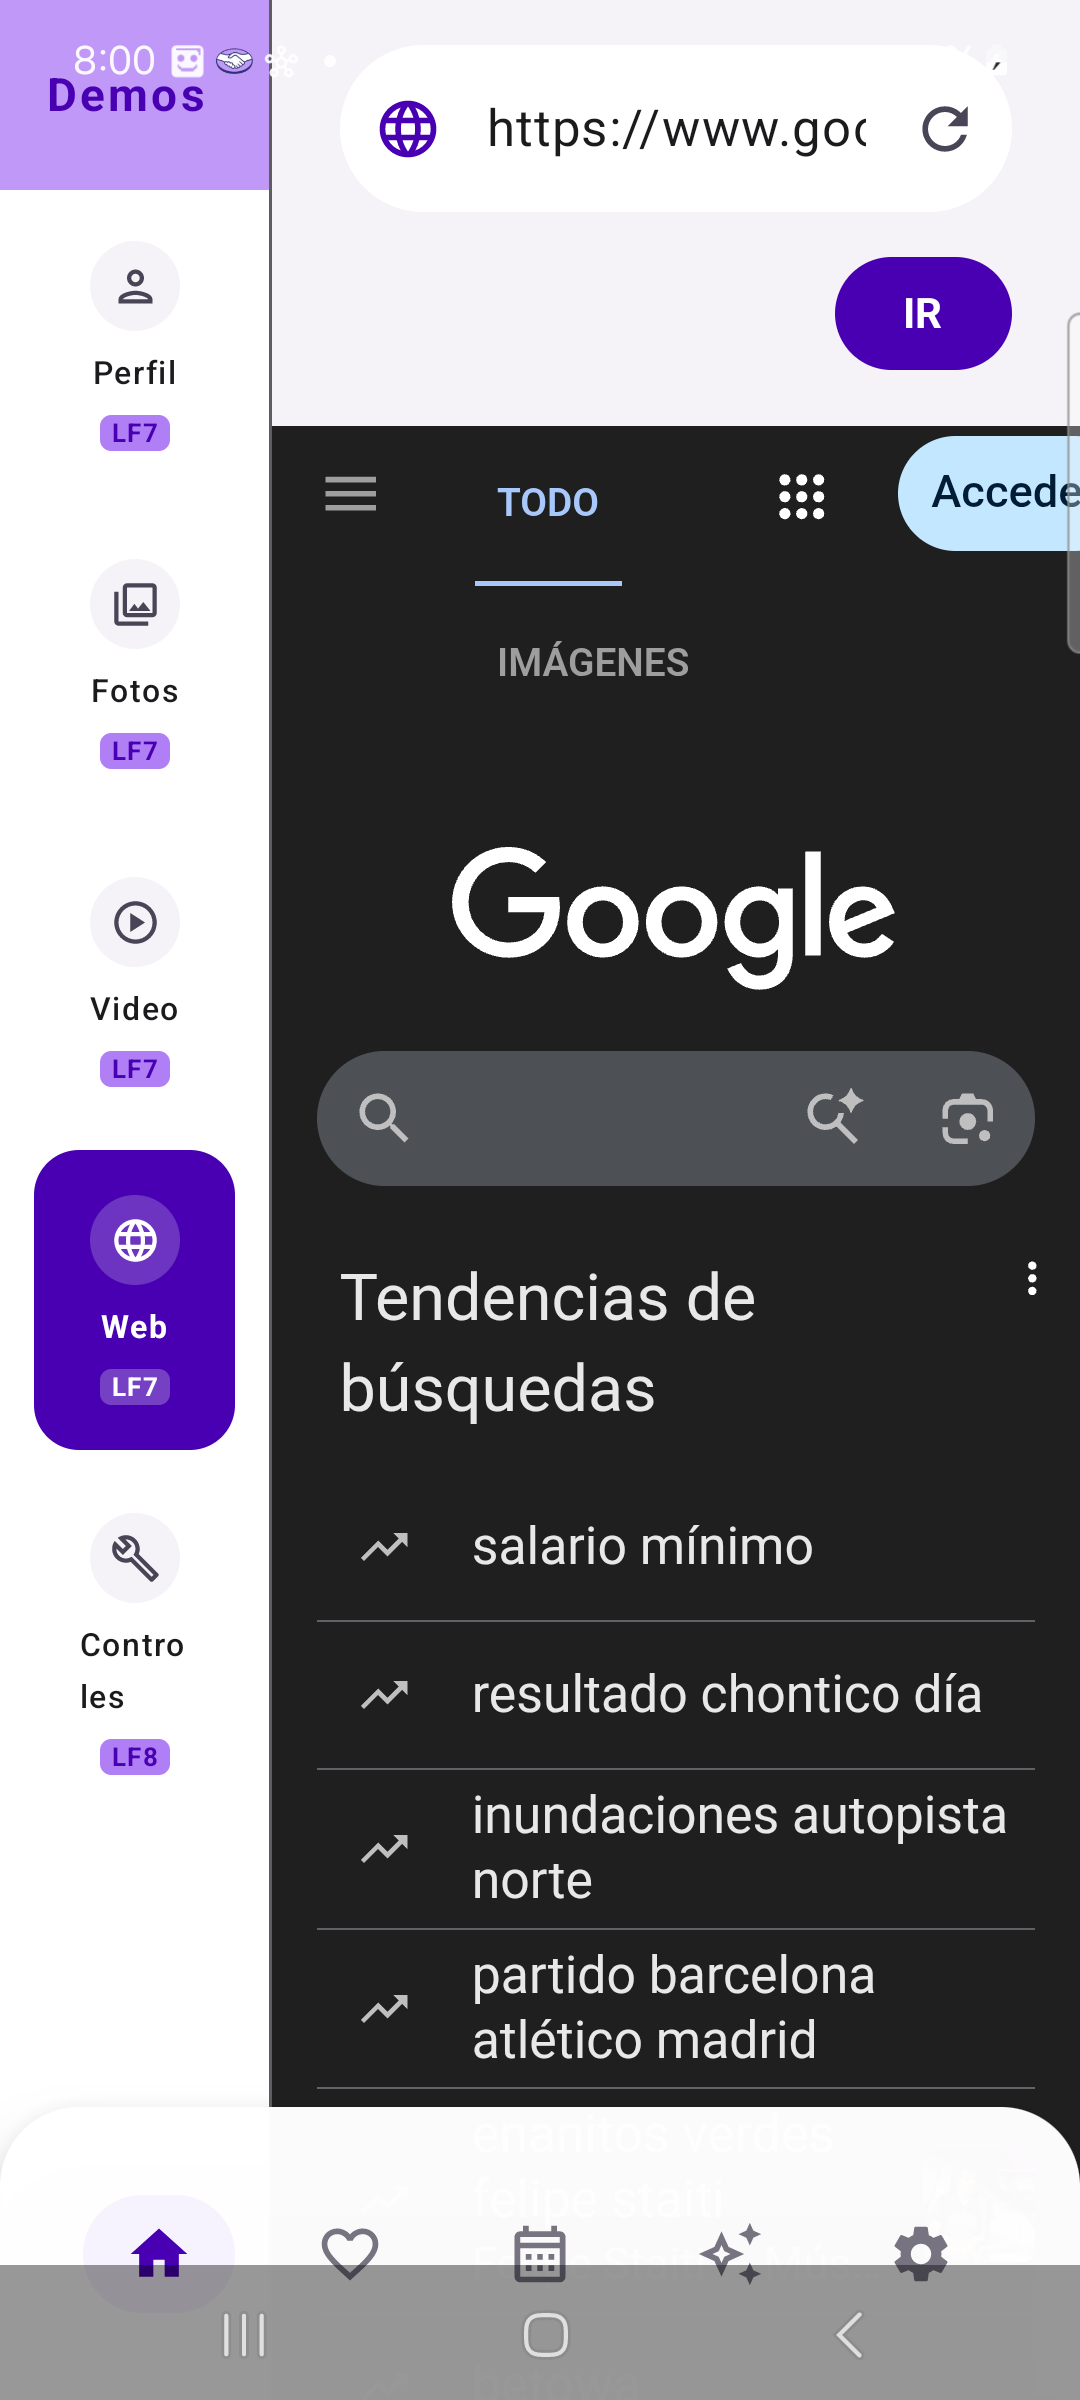
\includegraphics[width=0.30\textwidth]{screenshot_web.png}
\caption{Panel derecho Web --- navegador integrado con campo de URL, botón IR y WebView
renderizando página web. Elaboración propia.}
\label{fig:ss_web}
\end{figure}

\textbf{Panel derecho $\rightarrow$ Controles (ControlsScreen)}

\texttt{Column} con \texttt{verticalScroll} que organiza todos los controles en secciones
\texttt{ControlSection} (cada una es una \texttt{Card}):

\begin{longtable}{@{}p{3.5cm}p{12cm}@{}}
\caption{Secciones de controles implementados en ControlsScreen}
\label{tab:controlssecciones}\\
\toprule
\textbf{Sección} & \textbf{Controles} \\
\midrule
\endfirsthead
\toprule
\textbf{Sección} & \textbf{Controles} \\
\midrule
\endhead
\midrule
\multicolumn{2}{r}{\small\textit{Continúa en la página siguiente}}\\
\endfoot
\bottomrule
\endlastfoot
Botones & \texttt{Button} estándar + \texttt{ElevatedButton} \\[3pt]
Botón de ícono & \texttt{IconButton} con \texttt{Icon} (favorito on/off) \\[3pt]
Casillas de verificación & 3 \texttt{Checkbox} con etiquetas (Sin Gluten, Vegetariano,
Bajo en calorías) \\[3pt]
Selección única & \texttt{RadioButton} group con 3 opciones (Vegetariano, Omnívoro,
Vegano) \\[3pt]
Interruptor & \texttt{Switch} (Modo oscuro activado/desactivado) \\[3pt]
Menú desplegable & \texttt{ExposedDropdownMenuBox} con 5 categorías de receta \\[3pt]
Nivel de dificultad & \texttt{Slider} de 1 a 3 pasos con etiquetas Fácil/Medio/Difícil \\
\end{longtable}

Incluye un panel de resultado (\texttt{Box} con fondo \texttt{SecondaryContainer}) que
muestra el estado actual de todos los controles, y un botón ``CONFIRMAR Y VER RESULTADO''
de ancho completo al fondo de la pantalla.

\begin{figure}[H]
\centering
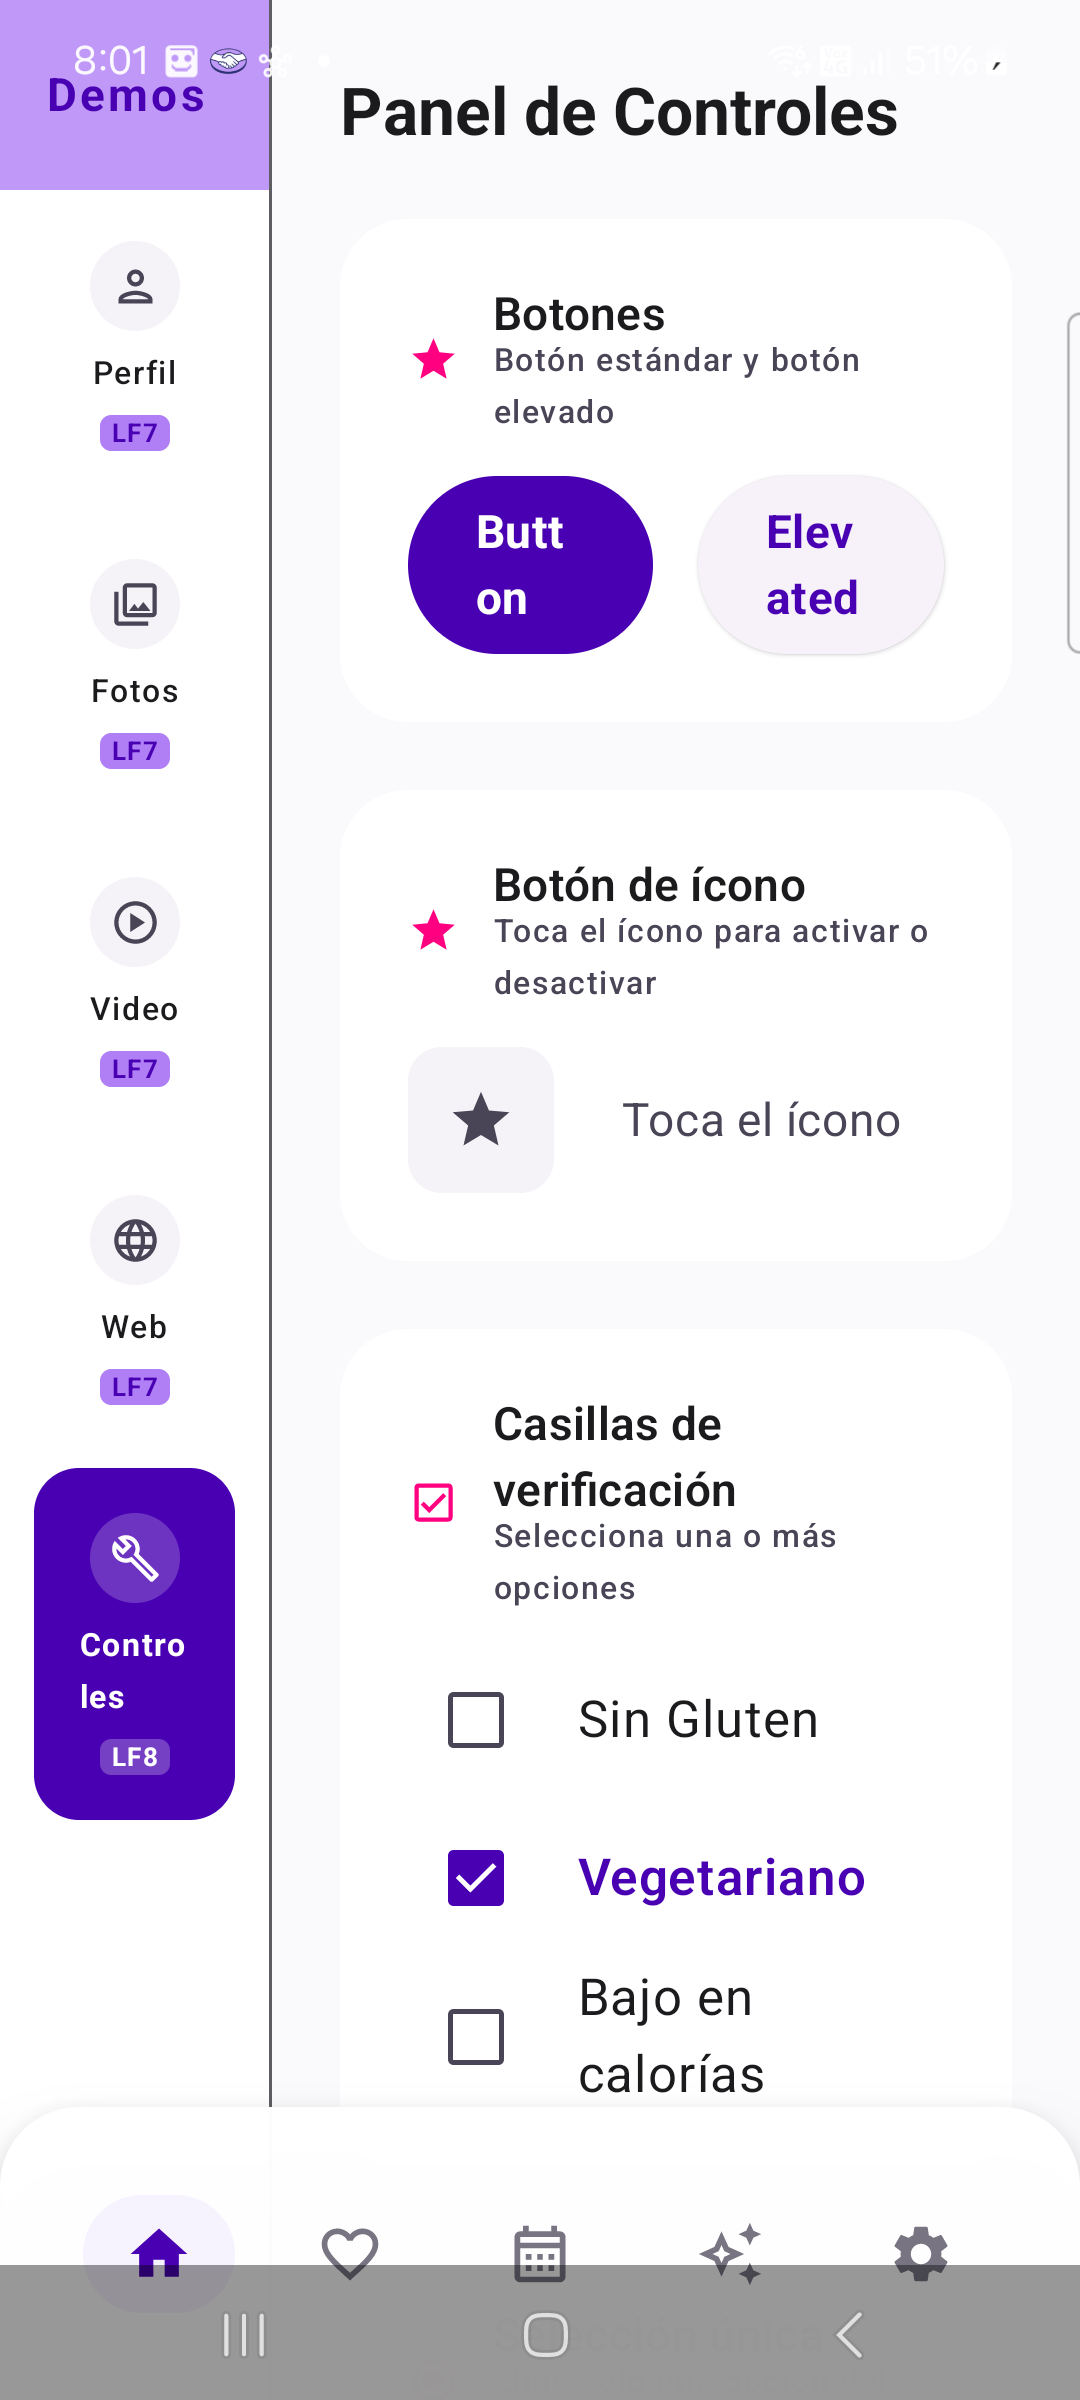
\includegraphics[width=0.30\textwidth]{screenshot_controls.png}
\caption{Panel derecho Controles --- demostración de Button, Checkbox, RadioButton,
Switch, Slider y Dropdown con panel de resultado. Elaboración propia.}
\label{fig:ss_controls}
\end{figure}

%+---------------------------------------------------------------+
\subsection{Asignación de identificadores y propiedades para cada vista}
\label{sec:identificadores}

En Jetpack Compose los elementos visuales no tienen atributos \texttt{android:id} como en
XML clásico. En su lugar, cada vista se identifica mediante el nombre de la variable de
estado que la controla o el nombre del composable que la define, y sus propiedades se
configuran a través del encadenamiento de \texttt{Modifier} y los parámetros de la
función. Los dos archivos XML que sí existen en la aplicación
(\texttt{activity\_main.xml} y \texttt{fragment\_global\_recipe\_search.xml}) mantienen el
esquema tradicional de identificadores.

\subsubsection{activity\_main.xml --- Identificadores XML}

\begin{table}[H]
\caption{Identificadores XML en activity\_main.xml}
\label{tab:idactivitymain}
\begin{tabularx}{\textwidth}{@{}p{3.5cm}p{3cm}X@{}}
\toprule
\textbf{ID (android:id)} & \textbf{Tipo de vista} & \textbf{Propiedades clave} \\
\midrule
\texttt{@+id/nav\_host\_fragment} & \texttt{FragmentContainerView} &
\texttt{layout\_width="match\_parent"}, \texttt{layout\_height="match\_parent"},
\texttt{app:navGraph="@navigation/main\_nav\_graph"},
\texttt{app:defaultNavHost="true"} \\
\bottomrule
\end{tabularx}
\end{table}

\subsubsection{fragment\_global\_recipe\_search.xml --- Identificadores XML}

\begin{table}[H]
\caption{Identificadores XML en fragment\_global\_recipe\_search.xml}
\label{tab:idfragmentsearch}
\begin{tabularx}{\textwidth}{@{}p{6cm}p{2.5cm}X@{}}
\toprule
\textbf{ID (android:id)} & \textbf{Tipo de vista} & \textbf{Propiedades clave} \\
\midrule
\texttt{@+id/globalRecipeSearchComposeView} & \texttt{ComposeView} &
\texttt{layout\_width="match\_parent"}, \texttt{layout\_height="match\_parent"} \\
\bottomrule
\end{tabularx}
\end{table}

\subsubsection{MainActivity --- Vistas Compose}

\begin{longtable}{@{}p{2.5cm}p{4.5cm}p{8.5cm}@{}}
\caption{Identificadores y propiedades de vistas Compose en MainActivity}
\label{tab:idmainactivity}\\
\toprule
\textbf{Identificador} & \textbf{Tipo Compose} & \textbf{Propiedades clave} \\
\midrule
\endfirsthead
\toprule
\textbf{Identificador} & \textbf{Tipo Compose} & \textbf{Propiedades clave} \\
\midrule
\endhead
\midrule
\multicolumn{3}{r}{\small\textit{Continúa en la página siguiente}}\\
\endfoot
\bottomrule
\endlastfoot
\texttt{LoadingBox} & \texttt{Box} & \texttt{fillMaxSize()}, \texttt{contentAlignment = Center}, \texttt{background(colorScheme.background)} \\[3pt]
\texttt{CircularProgressIndicator} & \texttt{CircularProgressIndicator} & Sin modificador adicional, centrado por el \texttt{Box} padre \\[3pt]
\texttt{AppContent} & \texttt{@Composable} & Aplica \texttt{RecipeGeneratorTheme(darkTheme = darkTheme)} \\[3pt]
\texttt{darkTheme} & \texttt{Boolean} (estado derivado) & Derivado de \texttt{prefs.theme == "Oscuro"} observado con \texttt{collectAsState} \\
\end{longtable}

\subsubsection{RecipeDetailActivity --- Vistas Compose}

\begin{longtable}{@{}p{2.5cm}p{5cm}p{8cm}@{}}
\caption{Identificadores y propiedades de vistas Compose en RecipeDetailActivity}
\label{tab:idrecipedetail}\\
\toprule
\textbf{Identificador} & \textbf{Tipo Compose} & \textbf{Propiedades clave} \\
\midrule
\endfirsthead
\toprule
\textbf{Identificador} & \textbf{Tipo Compose} & \textbf{Propiedades clave} \\
\midrule
\endhead
\midrule
\multicolumn{3}{r}{\small\textit{Continúa en la página siguiente}}\\
\endfoot
\bottomrule
\endlastfoot
\texttt{\_recipe} & \texttt{MutableStateFlow<Recipe?>} & Estado principal; \texttt{null} = pantalla vacía \\[3pt]
\texttt{\_isFavorite} & \texttt{MutableStateFlow<Boolean>} & Controla color del botón de favorito \\[3pt]
\texttt{\_videoUiState} & \texttt{MutableStateFlow<RecipeVideoUiState>} & Estados: Loading, Ready, Error, Empty \\[3pt]
\texttt{RecipeDetailScreen} & \texttt{@Composable} & Recibe \texttt{recipe}, \texttt{isFavorite}, \texttt{videoUiState}, \texttt{onToggleFavorite}, \texttt{onBackClick} \\
\end{longtable}

\subsubsection{HomeFragment $\rightarrow$ RecipeListScreen --- Vistas Compose}

\begin{longtable}{@{}p{2.5cm}p{4cm}p{9cm}@{}}
\caption{Identificadores y propiedades de vistas Compose en HomeFragment}
\label{tab:idhome}\\
\toprule
\textbf{Identificador} & \textbf{Tipo Compose} & \textbf{Propiedades clave} \\
\midrule
\endfirsthead
\toprule
\textbf{Identificador} & \textbf{Tipo Compose} & \textbf{Propiedades clave} \\
\midrule
\endhead
\midrule
\multicolumn{3}{r}{\small\textit{Continúa en la página siguiente}}\\
\endfoot
\bottomrule
\endlastfoot
\texttt{selectedDay} & \texttt{StateFlow<String>} & Día activo en la \texttt{ScrollableTabRow}; observable con \texttt{collectAsStateWithLifecycle} \\[3pt]
\texttt{recipes} & \texttt{StateFlow<List<Recipe>{}>} & Lista mostrada en la \texttt{LazyColumn} \\[3pt]
\texttt{favoriteRecipeIds} & \texttt{Set<String>} & Controla el estado del ícono de favorito por receta \\[3pt]
\texttt{TopAppBar} & \texttt{CenterAlignedTopAppBar} & \texttt{title = "RecipeGenerator"}, \texttt{actions = \{ IconButton(perfil) \}} \\[3pt]
Pestañas de días & \texttt{ScrollableTabRow} & \texttt{selectedTabIndex = selectedDay}, tabs generadas con \texttt{.forEachIndexed} \\[3pt]
Lista de recetas & \texttt{LazyColumn} & \texttt{fillMaxSize()}, \texttt{verticalArrangement = spacedBy(8.dp)} \\[3pt]
Tarjeta de receta & \texttt{Card} & \texttt{fillMaxWidth()}, \texttt{elevation = 2.dp}, \texttt{onClick = onRecipeSelected} \\[3pt]
Botón favorito & \texttt{IconButton} & \texttt{Icon(Favorite / FavoriteBorder)}, tint cambia con \texttt{animateColorAsState} \\[3pt]
Barra navegación & \texttt{NavigationBar} & 4 ítems: Inicio, Favoritos, Generador, Ajustes \\[3pt]
Indicador sync & \texttt{LinearProgressIndicator} & \texttt{fillMaxWidth()}, visible solo cuando \texttt{isSyncing == true} \\
\end{longtable}

\subsubsection{FavoritesFragment $\rightarrow$ FavoritesScreen --- Vistas Compose}

\begin{longtable}{@{}p{2.5cm}p{4cm}p{9cm}@{}}
\caption{Identificadores y propiedades de vistas Compose en FavoritesFragment}
\label{tab:idfavorites}\\
\toprule
\textbf{Identificador} & \textbf{Tipo Compose} & \textbf{Propiedades clave} \\
\midrule
\endfirsthead
\toprule
\textbf{Identificador} & \textbf{Tipo Compose} & \textbf{Propiedades clave} \\
\midrule
\endhead
\midrule
\multicolumn{3}{r}{\small\textit{Continúa en la página siguiente}}\\
\endfoot
\bottomrule
\endlastfoot
\texttt{searchQuery} & \texttt{StateFlow<String>} & Texto del campo de búsqueda; actualizado con \texttt{onSearchQueryChanged} \\[3pt]
\texttt{selectedCategory} & \texttt{StateFlow<String>} & Categoría activa del filtro; valor inicial ``Todos'' \\[3pt]
\texttt{filteredRecipes} & \texttt{StateFlow<List<Recipe>{}>} & Lista filtrada por texto + categoría \\[3pt]
Campo de búsqueda & \texttt{OutlinedTextField} & \texttt{value = searchQuery}, \texttt{leadingIcon = Search}, \texttt{singleLine = true}, \texttt{fillMaxWidth()} \\[3pt]
Filtros categoría & \texttt{LazyRow + FilterChip} & \texttt{horizontalArrangement = spacedBy(8.dp)}, \texttt{selected = selectedCategory == it} \\[3pt]
Lista favoritos & \texttt{LazyColumn} & \texttt{fillMaxSize()}, ítems con \texttt{key = \{ it.id \}} \\[3pt]
Botón eliminar & \texttt{IconButton} & \texttt{Icon(Delete)}, \texttt{onClick = onRemoveFavorite(recipe.id)} \\[3pt]
Estado vacío & \texttt{Column} & \texttt{fillMaxSize()}, \texttt{horizontalAlignment = Center}, ícono + texto descriptivo \\
\end{longtable}

\subsubsection{MenuGeneratorFragment $\rightarrow$ MenuGeneratorScreen --- Vistas Compose}

\begin{longtable}{@{}p{2.5cm}p{5cm}p{8cm}@{}}
\caption{Identificadores y propiedades de vistas Compose en MenuGeneratorFragment}
\label{tab:idgenerator}\\
\toprule
\textbf{Identificador} & \textbf{Tipo Compose} & \textbf{Propiedades clave} \\
\midrule
\endfirsthead
\toprule
\textbf{Identificador} & \textbf{Tipo Compose} & \textbf{Propiedades clave} \\
\midrule
\endhead
\midrule
\multicolumn{3}{r}{\small\textit{Continúa en la página siguiente}}\\
\endfoot
\bottomrule
\endlastfoot
\texttt{selectedDiets} & \texttt{StateFlow<Set<String>{}>} & Dietas activas; múltiple selección \\[3pt]
\texttt{maxDifficulty} & \texttt{StateFlow<String>} & Dificultad máxima seleccionada \\[3pt]
\texttt{portions} & \texttt{StateFlow<Int>} & Número de porciones (valor entre 1 y 10) \\[3pt]
\texttt{selectedTypes} & \texttt{StateFlow<Set<String>{}>} & Tipos de receta activos \\[3pt]
\texttt{uiState} & \texttt{StateFlow<MenuGeneratorUiState>} & Estados: Idle, Loading, Success, Error \\[3pt]
Chips de dieta & \texttt{FilterChip} & \texttt{selected = it in selectedDiets}, \texttt{onClick = onToggleDiet(it)} \\[3pt]
Selector dificultad & \texttt{SingleChoiceSegmentedButtonRow} & Opciones: Fácil / Medio / Difícil \\[3pt]
Control porciones & \texttt{Row} & \texttt{IconButton("-")} + \texttt{Text(portions)} + \texttt{IconButton("+")}, \texttt{verticalAlignment = Center} \\[3pt]
Chips tipo receta & \texttt{FilterChip} & \texttt{selected = it in selectedTypes}, \texttt{onClick = onToggleRecipeType(it)} \\[3pt]
Botón generar & \texttt{Button} & \texttt{fillMaxWidth()}, \texttt{height = 56.dp}, \texttt{onClick = onGenerateClick}, \texttt{enabled = uiState != Loading} \\[3pt]
Modal resultado & \texttt{ModalBottomSheet} & Muestra plan generado; \texttt{onDismissRequest = cerrar modal} \\
\end{longtable}

\subsubsection{SettingsFragment $\rightarrow$ SettingsScreen --- Vistas Compose}

\begin{longtable}{@{}p{2.5cm}p{4cm}p{9cm}@{}}
\caption{Identificadores y propiedades de vistas Compose en SettingsFragment}
\label{tab:idsettings}\\
\toprule
\textbf{Identificador} & \textbf{Tipo Compose} & \textbf{Propiedades clave} \\
\midrule
\endfirsthead
\toprule
\textbf{Identificador} & \textbf{Tipo Compose} & \textbf{Propiedades clave} \\
\midrule
\endhead
\midrule
\multicolumn{3}{r}{\small\textit{Continúa en la página siguiente}}\\
\endfoot
\bottomrule
\endlastfoot
\texttt{preferences} & \texttt{StateFlow<UserPreferences>} & Estado global de ajustes del usuario \\[3pt]
\texttt{selectedTheme} & \texttt{String} derivado & Valor: ``Claro'' o ``Oscuro'' \\[3pt]
\texttt{selectedLanguage} & \texttt{String} derivado & Valor: ``Español'' o ``English'' \\[3pt]
\texttt{defaultPortions} & \texttt{Int} derivado & Entre 1 y 10 \\[3pt]
Cards de tema & \texttt{Card} ($\times$2) & \texttt{onClick = onThemeSelect(it)}, borde primario si está seleccionada \\[3pt]
Chips dietas & \texttt{FilterChip} & \texttt{selected = it in selectedDiets}, \texttt{onClick = onToggleDiet(it)} \\[3pt]
Control porciones & \texttt{Row} & \texttt{IconButton("-")} + \texttt{Text} + \texttt{IconButton("+")} \\[3pt]
Cards idioma & \texttt{Card} ($\times$2) & \texttt{onClick = onLanguageSelect(it)}, borde primario si activa \\[3pt]
Botón cerrar sesión & \texttt{TextButton} & \texttt{fillMaxWidth()}, \texttt{contentColor = Error}, \texttt{icon = Logout} \\
\end{longtable}

\subsubsection{LeftMenuFragment $\rightarrow$ MainScreen --- Layout de dos paneles}

\begin{longtable}{@{}p{2.5cm}p{5.5cm}p{7.5cm}@{}}
\caption{Identificadores y propiedades del layout de dos paneles en LeftMenuFragment}
\label{tab:idleftmenu}\\
\toprule
\textbf{Identificador} & \textbf{Tipo Compose} & \textbf{Propiedades clave} \\
\midrule
\endfirsthead
\toprule
\textbf{Identificador} & \textbf{Tipo Compose} & \textbf{Propiedades clave} \\
\midrule
\endhead
\midrule
\multicolumn{3}{r}{\small\textit{Continúa en la página siguiente}}\\
\endfoot
\bottomrule
\endlastfoot
\texttt{selectedPanel} & \texttt{var by remember \{ mutableStateOf(LeftMenuPanel.Profile) \}} & Estado local que controla qué composable se muestra en el panel derecho; tipo: \texttt{LeftMenuPanel} (enum) \\[3pt]
Contenedor raíz & \texttt{Box} & \texttt{modifier.fillMaxSize()} \\[3pt]
Fila principal & \texttt{Row} & \texttt{fillMaxSize()} \\[3pt]
Panel izquierdo & \texttt{LeftMenuScreen} & \texttt{weight(0.25f)}, \texttt{fillMaxHeight()} \\[3pt]
Divisor vertical & \texttt{Box} & \texttt{width(1.dp)}, \texttt{fillMaxHeight()}, \texttt{background(OutlineVariant.copy(alpha=0.3f))} \\[3pt]
Panel derecho & \texttt{Box} & \texttt{weight(0.75f)}, \texttt{fillMaxHeight()} \\[3pt]
TopAppBar superpuesto & \texttt{DetailEditorialTopAppBar} & Título ``Pantallas Demo'', \texttt{leadingContent = \{ IconButton(ArrowBack) \}} \\
\end{longtable}

\subsubsection{LeftMenuScreen --- Panel izquierdo}

\begin{longtable}{@{}p{2.5cm}p{4cm}p{9cm}@{}}
\caption{Identificadores y propiedades del panel izquierdo LeftMenuScreen}
\label{tab:idleftmenuscreen}\\
\toprule
\textbf{Identificador} & \textbf{Tipo Compose} & \textbf{Propiedades clave} \\
\midrule
\endfirsthead
\toprule
\textbf{Identificador} & \textbf{Tipo Compose} & \textbf{Propiedades clave} \\
\midrule
\endhead
\midrule
\multicolumn{3}{r}{\small\textit{Continúa en la página siguiente}}\\
\endfoot
\bottomrule
\endlastfoot
Contenedor & \texttt{Column} & \texttt{fillMaxHeight()}, \texttt{background(SurfaceContainerLowest)} \\[3pt]
Encabezado & \texttt{Box} & \texttt{fillMaxWidth()}, \texttt{background(PrimaryContainer.copy(alpha=0.4f))} \\[3pt]
Texto ``Demos'' & \texttt{Text} & \texttt{style = titleSmall}, \texttt{color = Primary}, \texttt{fontWeight = Bold} \\[3pt]
Lista de opciones & \texttt{LazyColumn} & \texttt{fillMaxWidth()}, \texttt{weight(1f)}, \texttt{verticalArrangement = spacedBy(2.dp)} \\[3pt]
Contenedor ítem & \texttt{Box} & \texttt{fillMaxWidth()}, \texttt{clip(RoundedCornerShape(rounded\_md))}, \texttt{background(bgColor)}, \texttt{clickable(onClick)} \\[3pt]
\texttt{bgColor} & \texttt{animateColorAsState} & \texttt{targetValue = if (isSelected) Primary else Transparent}, \texttt{animationSpec = tween(200)} \\[3pt]
\texttt{textColor} & \texttt{animateColorAsState} & \texttt{targetValue = if (isSelected) OnPrimary else OnSurface} \\[3pt]
\texttt{iconColor} & \texttt{animateColorAsState} & \texttt{targetValue = if (isSelected) OnPrimary else OnSurfaceVariant} \\[3pt]
Círculo ícono & \texttt{Box} & \texttt{size(32.dp)}, \texttt{background(color, CircleShape)} \\[3pt]
Ícono & \texttt{Icon} & \texttt{imageVector = panel.icon}, \texttt{tint = iconColor}, \texttt{size(18.dp)} \\[3pt]
Etiqueta & \texttt{Text} & \texttt{style = labelSmall}, \texttt{color = textColor}, \texttt{fontSize = 10.sp} \\[3pt]
Badge & \texttt{Box} & \texttt{background(color, RoundedCornerShape(4.dp))}, \texttt{padding(horizontal=4.dp, vertical=1.dp)} \\
\end{longtable}

\noindent\textbf{Enum LeftMenuPanel --- valores e identificadores:}

\begin{table}[H]
\caption{Valores del enum LeftMenuPanel con etiquetas, íconos y tags}
\label{tab:enumleftmenu}
\begin{tabularx}{\textwidth}{@{}llXl@{}}
\toprule
\textbf{Valor enum} & \textbf{label} & \textbf{icon} & \textbf{tag} \\
\midrule
Profile & ``Perfil'' & \texttt{Icons.Outlined.Person} & ``LF7'' \\[3pt]
Photos & ``Fotos'' & \texttt{Icons.Outlined.PhotoLibrary} & ``LF7'' \\[3pt]
Video & ``Video'' & \texttt{Icons.Outlined.PlayCircle} & ``LF7'' \\[3pt]
Web & ``Web'' & \texttt{Icons.Outlined.Language} & ``LF7'' \\[3pt]
Controls & ``Controles'' & \texttt{Icons.Outlined.Build} & ``LF8'' \\
\bottomrule
\end{tabularx}
\end{table}

%+---------------------------------------------------------------+
\subsection{Definición de variables y vínculos de estas con los identificadores}
\label{sec:variables}

En Android tradicional (XML + Java/Kotlin), las variables se declaran en la clase del
Fragment o Activity y se vinculan a las vistas mediante \texttt{findViewById()}. En
Jetpack Compose, el vínculo es directo y reactivo: la variable de estado es el
identificador de la vista, y cualquier cambio en ella dispara automáticamente la
recomposición de la interfaz. A continuación se documenta cada esquema según corresponda.

\subsubsection{activity\_main.xml --- Vínculo XML tradicional}

El único vínculo XML clásico de la app ocurre en \texttt{GlobalRecipeSearchFragment},
donde se obtiene la vista por su id para luego inyectar contenido Compose:

\begin{lstlisting}[caption={Vínculo XML tradicional en GlobalRecipeSearchFragment.kt}]
class GlobalRecipeSearchFragment : Fragment() {

    // Variable que referencia el ComposeView definido en el XML
    // Se vincula al id: R.id.globalRecipeSearchComposeView
    private lateinit var composeView: ComposeView

    override fun onCreateView(...): View {
        // Infla el layout XML (fragment_global_recipe_search.xml)
        return inflater.inflate(
            R.layout.fragment_global_recipe_search, container, false
        )
    }

    override fun onViewCreated(view: View, savedInstanceState: Bundle?) {
        super.onViewCreated(view, savedInstanceState)

        // Vinculo de la variable con el identificador XML
        composeView = view.findViewById(
            R.id.globalRecipeSearchComposeView
        )

        composeView.setViewCompositionStrategy(
            ViewCompositionStrategy.DisposeOnViewTreeLifecycleDestroyed
        )
        composeView.setContent {
            GlobalRecipeSearchScreen(
                onBack = { findNavController().navigateUp() }
            )
        }
    }
}
\end{lstlisting}

\subsubsection{ComposeScreenFragment --- Vínculo programático del ComposeView}

Los fragments que extienden \texttt{ComposeScreenFragment} no usan
\texttt{findViewById}. En su lugar, la variable \texttt{ComposeView} se crea y vincula
programáticamente en \texttt{onCreateView}:

\begin{lstlisting}[caption={Vínculo programático en ComposeScreenFragment.kt}]
abstract class ComposeScreenFragment : Fragment() {

    protected val appContainer
        get() = (requireActivity().application
            as RecipeGeneratorApp).container

    override fun onCreateView(
        inflater: LayoutInflater,
        container: ViewGroup?,
        savedInstanceState: Bundle?
    ): View {
        // Variable local creada sin XML - vinculo programatico
        val composeView = ComposeView(requireContext())

        composeView.setViewCompositionStrategy(
            ViewCompositionStrategy.DisposeOnViewTreeLifecycleDestroyed
        )

        composeView.setContent {
            val preferences by userPrefsRepository
                .getUserPreferences()
                .collectAsStateWithLifecycle(
                    initialValue = UserPreferences()
                )

            RecipeGeneratorTheme(
                darkTheme = preferences.theme == "Oscuro"
            ) {
                ScreenContent()
            }
        }

        return composeView
    }

    @Composable
    protected abstract fun ScreenContent()
}
\end{lstlisting}

\subsubsection{MainActivity --- Variables y vínculos}

\begin{lstlisting}[caption={Variables y vínculos en MainActivity.kt}]
class MainActivity : AppCompatActivity() {

    override fun onCreate(savedInstanceState: Bundle?) {
        super.onCreate(savedInstanceState)
        enableEdgeToEdge()
        setContent { AppContent() }
    }

    @Composable
    private fun AppContent() {
        val container = (application as RecipeGeneratorApp).container

        // Variable 'prefs' vinculada al flujo de preferencias
        val prefs by container.userPrefsRepository
            .getUserPreferences()
            .collectAsState(initial = UserPreferences())

        // Variable booleana derivada - controla el tema visual
        val darkTheme = prefs.theme == "Oscuro"

        RecipeGeneratorTheme(darkTheme = darkTheme) {
            AppContentInner()
        }
    }

    @Composable
    private fun AppContentInner() {
        val container = (application as RecipeGeneratorApp).container
        val authViewModel: AuthViewModel = viewModel(
            factory = AuthViewModelFactory(container.authRepository)
        )

        val isCheckingAuth by authViewModel.isCheckingAuth
            .collectAsState()
        val currentUser by authViewModel.currentUser
            .collectAsState()

        var wasAlreadyLoggedIn by remember {
            mutableStateOf<Boolean?>(null)
        }
        var welcomeSeen by remember { mutableStateOf(false) }

        when {
            isCheckingAuth -> LoadingBox()
            currentUser == null -> AuthScreen(
                viewModel = authViewModel, ...
            )
            wasAlreadyLoggedIn == false && !welcomeSeen ->
                AuthWelcomeScreen(...)
            else -> AppShell(...)
        }
    }
}
\end{lstlisting}

\subsubsection{RecipeDetailActivity --- Variables y vínculos}

\begin{lstlisting}[caption={Variables y vínculos en RecipeDetailActivity.kt}]
class RecipeDetailActivity : AppCompatActivity() {

    override fun onCreate(savedInstanceState: Bundle?) {
        super.onCreate(savedInstanceState)
        enableEdgeToEdge()

        // Variable que recibe el ID desde el Intent
        val recipeId = intent.getStringExtra(EXTRA_RECIPE_ID)
            ?: run { finish(); return }

        val container = (application as RecipeGeneratorApp).container
        val viewModel: DetailActivityViewModel = ViewModelProvider(
            this, DetailActivityViewModelFactory(...)
        )[DetailActivityViewModel::class.java]

        viewModel.loadRecipe(recipeId)

        setContent {
            val recipe = viewModel.recipe
                .collectAsStateWithLifecycle().value
            val isFavorite = viewModel.isFavorite
                .collectAsStateWithLifecycle().value
            val videoUiState = viewModel.videoUiState
                .collectAsStateWithLifecycle().value

            if (recipe != null) {
                RecipeDetailScreen(
                    recipe = recipe,
                    isFavorite = isFavorite,
                    videoUiState = videoUiState,
                    onToggleFavorite = { viewModel.toggleFavorite() },
                    onBackClick = {
                        onBackPressedDispatcher.onBackPressed()
                    }
                )
            }
        }
    }
}

// ViewModel - variables internas vinculadas a la UI
class DetailActivityViewModel(...) : ViewModel() {
    private val _recipe = MutableStateFlow<Recipe?>(null)
    val recipe: StateFlow<Recipe?> = _recipe.asStateFlow()

    private val _isFavorite = MutableStateFlow(false)
    val isFavorite: StateFlow<Boolean> = _isFavorite.asStateFlow()

    private val _videoUiState =
        MutableStateFlow<RecipeVideoUiState>(
            RecipeVideoUiState.Loading
        )
    val videoUiState: StateFlow<RecipeVideoUiState> =
        _videoUiState.asStateFlow()

    fun loadRecipe(recipeId: String) {
        viewModelScope.launch {
            getRecipeDetailUseCase(recipeId).collect { r ->
                _recipe.value = r
            }
        }
        viewModelScope.launch {
            favoritesRepository.getFavoriteIds(userId)
                .collect { ids ->
                    _isFavorite.value = recipeId in ids
                }
        }
    }
}
\end{lstlisting}

\subsubsection{HomeFragment --- Variables y vínculos}

\begin{lstlisting}[caption={Variables y vínculos en HomeFragment.kt}]
class HomeFragment : ComposeScreenFragment() {

    private val homeViewModel: HomeViewModel by viewModels {
        HomeViewModelFactory(
            appContainer.getMenuForDayUseCase, ...
        )
    }

    @Composable
    override fun ScreenContent() {
        val selectedDay by homeViewModel.selectedDay
            .collectAsStateWithLifecycle()
        val recipes by homeViewModel.recipes
            .collectAsStateWithLifecycle()
        val favoriteRecipeIds by appContainer.favoritesRepository
            .getFavoriteIds(userId)
            .collectAsStateWithLifecycle(
                initialValue = emptySet()
            )

        RecipeListScreen(
            selectedDay = selectedDay,
            recipes = recipes,
            favoriteRecipeIds = favoriteRecipeIds,
            onDaySelected = homeViewModel::selectDay,
            onRecipeSelected = { recipe ->
                startActivity(
                    RecipeDetailActivity.newIntent(
                        requireContext(), recipe.id
                    )
                )
            },
            onProfileClick = {
                findNavController().navigate(
                    R.id.action_home_to_leftMenu
                )
            }
        )
    }
}
\end{lstlisting}

\subsubsection{LeftMenuFragment $\rightarrow$ MainScreen --- Variables y vínculos}

\begin{lstlisting}[caption={Variables y vínculos en MainScreen.kt --- Layout de dos paneles}]
@Composable
fun MainScreen(modifier: Modifier = Modifier) {

    // Variable de estado local - identifica el panel activo
    var selectedPanel by remember {
        mutableStateOf(LeftMenuPanel.Profile)
    }

    Row(modifier = Modifier.fillMaxSize()) {
        // Panel izquierdo
        LeftMenuScreen(
            selectedPanel = selectedPanel,
            onPanelSelected = { selectedPanel = it },
            modifier = Modifier.weight(0.25f).fillMaxHeight()
        )

        // Divisor visual
        Box(modifier = Modifier.width(1.dp).fillMaxHeight()
            .background(OutlineVariant.copy(alpha = 0.3f)))

        // Panel derecho
        Box(modifier = Modifier.weight(0.75f).fillMaxHeight()) {
            when (selectedPanel) {
                LeftMenuPanel.Profile ->
                    ProfileHubScreen(Modifier.fillMaxSize())
                LeftMenuPanel.Photos ->
                    PhotosScreen(Modifier.fillMaxSize())
                LeftMenuPanel.Video ->
                    VideoScreen(Modifier.fillMaxSize())
                LeftMenuPanel.Web ->
                    WebScreen(Modifier.fillMaxSize())
                LeftMenuPanel.Controls ->
                    ControlsScreen(Modifier.fillMaxSize())
            }
        }
    }
}
\end{lstlisting}

\subsubsection{PhotosScreen --- Variables y vínculos}

\begin{lstlisting}[caption={Variables y vínculos en PhotosScreen.kt}]
@Composable
fun PhotosScreen(modifier: Modifier = Modifier) {

    val allRecipes by recipesFlow.collectAsStateWithLifecycle(
        initialValue = emptyList()
    )
    val galleryRecipes = remember(allRecipes) {
        allRecipes.take(10)
    }

    // Variable de estado local - ID de la receta seleccionada
    var selectedRecipeId by remember {
        mutableStateOf<String?>(null)
    }

    val selectedRecipe = remember(selectedRecipeId, galleryRecipes) {
        galleryRecipes.firstOrNull { it.id == selectedRecipeId }
    }

    // Color animado del panel de descripcion
    val descBg by animateColorAsState(
        targetValue = if (selectedRecipe != null)
            SecondaryContainer else Surface,
        animationSpec = tween(300), label = "descBg"
    )

    Column(modifier = modifier.fillMaxSize().background(Surface)) {
        if (selectedRecipe != null) {
            Box(Modifier.fillMaxWidth().background(descBg)
                .padding(spacing_6)) {
                Text(text = selectedRecipe.title, ...)
                Text(text = selectedRecipe.description, ...)
            }
        }

        LazyColumn {
            items(galleryRecipes, key = { it.id }) { recipe ->
                RecipePhotoCard(
                    recipe = recipe,
                    isSelected = recipe.id == selectedRecipeId,
                    onClick = {
                        selectedRecipeId =
                            if (selectedRecipeId == recipe.id)
                                null else recipe.id
                    }
                )
            }
        }
    }
}
\end{lstlisting}

\subsubsection{VideoScreen --- Variables y vínculos}

\begin{lstlisting}[caption={Variables y vínculos en VideoScreen.kt}]
@Composable
fun VideoScreen(modifier: Modifier = Modifier) {

    val context = LocalContext.current
    val lifecycleOwner = LocalLifecycleOwner.current

    var isLoading by remember { mutableStateOf(true) }
    var hasError by remember { mutableStateOf(false) }
    var videoViewRef by remember {
        mutableStateOf<VideoView?>(null)
    }

    DisposableEffect(lifecycleOwner) {
        val observer = LifecycleEventObserver { _, event ->
            when (event) {
                Lifecycle.Event.ON_PAUSE ->
                    videoViewRef?.pause()
                Lifecycle.Event.ON_RESUME ->
                    videoViewRef?.start()
                Lifecycle.Event.ON_DESTROY -> {
                    videoViewRef?.stopPlayback()
                    videoViewRef = null
                }
                else -> Unit
            }
        }
        lifecycleOwner.lifecycle.addObserver(observer)
        onDispose {
            lifecycleOwner.lifecycle.removeObserver(observer)
            videoViewRef?.stopPlayback()
        }
    }

    AndroidView(
        factory = { ctx ->
            VideoView(ctx).apply {
                val mc = MediaController(ctx)
                mc.setAnchorView(this)
                setMediaController(mc)
                setVideoURI(Uri.parse(
                    "android.resource://${ctx.packageName}" +
                    "/${R.raw.sample_video}"
                ))
                setOnPreparedListener { mp ->
                    isLoading = false
                    mp.isLooping = false
                }
                setOnErrorListener { _, _, _ ->
                    isLoading = false; hasError = true; false
                }
                requestFocus(); start()
            }
        },
        update = { videoView -> videoViewRef = videoView }
    )
}
\end{lstlisting}

\subsubsection{WebScreen --- Variables y vínculos}

\begin{lstlisting}[caption={Variables y vínculos en WebScreen.kt}]
@Composable
fun WebScreen(modifier: Modifier = Modifier) {

    var urlInput by remember {
        mutableStateOf("https://www.google.com")
    }
    var currentUrl by remember {
        mutableStateOf("https://www.google.com")
    }
    var isLoading by remember { mutableStateOf(false) }
    var webViewRef by remember {
        mutableStateOf<WebView?>(null)
    }

    OutlinedTextField(
        value = urlInput,
        onValueChange = { urlInput = it },
        trailingIcon = {
            IconButton(onClick = { webViewRef?.reload() })
            { Icon(Icons.Filled.Refresh, "Recargar") }
        }
    )

    Button(onClick = {
        val finalUrl = if (urlInput.startsWith("http"))
            urlInput else "https://${urlInput}"
        currentUrl = finalUrl
        webViewRef?.loadUrl(finalUrl)
    }) { Text("IR") }

    AndroidView(
        factory = { ctx ->
            WebView(ctx).apply {
                webViewClient = object : WebViewClient() {
                    override fun onPageStarted(...) {
                        isLoading = true
                    }
                    override fun onPageFinished(
                        view: WebView?, url: String?
                    ) {
                        isLoading = false
                        url?.let { urlInput = it }
                    }
                }
                webViewRef = this
                loadUrl(currentUrl)
            }
        },
        update = { webView -> webViewRef = webView }
    )
}
\end{lstlisting}

\subsubsection{ControlsScreen --- Variables y vínculos}

\begin{lstlisting}[caption={Variables y vínculos en ControlsScreen.kt}]
@Composable
fun ControlsScreen(modifier: Modifier = Modifier) {

    var isSwitchOn by remember { mutableStateOf(false) }
    var isCheckbox1 by remember { mutableStateOf(false) }
    var isCheckbox2 by remember { mutableStateOf(true) }
    var isCheckbox3 by remember { mutableStateOf(false) }
    var selectedRadio by remember {
        mutableStateOf("Omnivoro")
    }
    var sliderValue by remember { mutableFloatStateOf(2f) }
    var spinnerExpanded by remember { mutableStateOf(false) }
    var selectedCategory by remember {
        mutableStateOf("Almuerzo")
    }
    var resultText by remember { mutableStateOf("") }
    var iconToggle by remember { mutableStateOf(false) }

    // Cada variable controla directamente su composable:
    Button(onClick = {
        resultText = "Button presionado"
    }) { Text("Button") }

    Checkbox(checked = isCheckbox1, onCheckedChange = {
        isCheckbox1 = it
        resultText = buildCheckboxResult(
            isCheckbox1, isCheckbox2, isCheckbox3
        )
    })

    Switch(checked = isSwitchOn, onCheckedChange = {
        isSwitchOn = it
        resultText = "Switch: ${if (it) "ON" else "OFF"}"
    })

    Slider(
        value = sliderValue,
        onValueChange = {
            sliderValue = it
            resultText = "Nivel: ${when(it.toInt()) {
                1 -> "Facil"; 2 -> "Medio"
                else -> "Dificil"
            }}"
        },
        valueRange = 1f..3f, steps = 1
    )

    Button(onClick = {
        resultText = buildSummary(
            isSwitchOn, isCheckbox1, isCheckbox2,
            isCheckbox3, selectedRadio,
            sliderValue, selectedCategory
        )
    }) { Text("CONFIRMAR Y VER RESULTADO") }
}
\end{lstlisting}

%+---------------------------------------------------------------+
\subsection{Identificación de los eventos y declaración de los métodos de cada uno}
\label{sec:eventos}

En Android tradicional los eventos se registran con métodos como
\texttt{setOnClickListener\{\}} o \texttt{addTextChangedListener\{\}}. En Jetpack Compose
los eventos son parámetros lambda que se pasan directamente al composable
(\texttt{onClick}, \texttt{onValueChange}, \texttt{onCheckedChange}, etc.). Los eventos
de ciclo de vida se gestionan con \texttt{DisposableEffect} y \texttt{LaunchedEffect}.
A continuación se identifican todos los eventos de la aplicación con su método declarado.

\subsubsection{MainActivity --- Eventos y métodos}

\begin{longtable}{@{}p{2.5cm}p{4cm}p{9cm}@{}}
\caption{Eventos y métodos declarados en MainActivity}
\label{tab:evmainactivity}\\
\toprule
\textbf{Evento} & \textbf{Dónde ocurre} & \textbf{Método declarado} \\
\midrule
\endfirsthead
\toprule
\textbf{Evento} & \textbf{Dónde ocurre} & \textbf{Método declarado} \\
\midrule
\endhead
\midrule
\multicolumn{3}{r}{\small\textit{Continúa en la página siguiente}}\\
\endfoot
\bottomrule
\endlastfoot
App iniciada & \texttt{onCreate()} & Llama \texttt{setContent \{\}} y \texttt{enableEdgeToEdge()} \\[3pt]
Cambio de sesión & \texttt{LaunchedEffect(currentUser)} & Detecta si el usuario ya estaba logueado al arrancar \\[3pt]
Login exitoso & \texttt{onAuthSuccess} callback & Establece \texttt{wasAlreadyLoggedIn = false} \\[3pt]
Recuperación de red & \texttt{connectivityObserver.observe()} & Dispara re-sincronización con Firestore \\[3pt]
Click en ``Cerrar sesión'' & \texttt{handleLogout} lambda & Limpia datos locales y llama \texttt{authViewModel.logout()} \\
\end{longtable}

\subsubsection{RecipeDetailActivity --- Eventos y métodos}

\begin{longtable}{@{}p{2.5cm}p{4cm}p{9cm}@{}}
\caption{Eventos y métodos declarados en RecipeDetailActivity}
\label{tab:evrecipedetail}\\
\toprule
\textbf{Evento} & \textbf{Dónde ocurre} & \textbf{Método declarado} \\
\midrule
\endfirsthead
\toprule
\textbf{Evento} & \textbf{Dónde ocurre} & \textbf{Método declarado} \\
\midrule
\endhead
\midrule
\multicolumn{3}{r}{\small\textit{Continúa en la página siguiente}}\\
\endfoot
\bottomrule
\endlastfoot
Activity creada & \texttt{onCreate()} & Lee \texttt{EXTRA\_RECIPE\_ID} del \texttt{Intent} y carga la receta \\[3pt]
Click en favorito & \texttt{onToggleFavorite} lambda & Llama \texttt{viewModel.toggleFavorite()} \\[3pt]
Click en volver & \texttt{onBackClick} lambda & Llama \texttt{onBackPressedDispatcher.onBackPressed()} \\[3pt]
Receta cargada & \texttt{loadRecipe()} $\rightarrow$ \texttt{collect \{\}} & Actualiza \texttt{\_recipe.value} \\[3pt]
Favorito cambia & \texttt{getFavoriteIds().collect \{\}} & Actualiza \texttt{\_isFavorite.value} \\[3pt]
Video resuelto & \texttt{cacheVideoIfNeeded()} & Actualiza \texttt{\_videoUiState.value} \\
\end{longtable}

\subsubsection{HomeFragment --- Eventos y métodos}

\begin{longtable}{@{}p{2.5cm}p{4cm}p{9cm}@{}}
\caption{Eventos y métodos declarados en HomeFragment}
\label{tab:evhome}\\
\toprule
\textbf{Evento} & \textbf{Dónde ocurre} & \textbf{Método declarado} \\
\midrule
\endfirsthead
\toprule
\textbf{Evento} & \textbf{Dónde ocurre} & \textbf{Método declarado} \\
\midrule
\endhead
\midrule
\multicolumn{3}{r}{\small\textit{Continúa en la página siguiente}}\\
\endfoot
\bottomrule
\endlastfoot
Click en pestaña de día & \texttt{onDaySelected} lambda & \texttt{homeViewModel::selectDay} \\[3pt]
Click en una receta & \texttt{onRecipeSelected} lambda & Lanza \texttt{RecipeDetailActivity} con \texttt{newIntent()} \\[3pt]
Click en favorito & \texttt{onToggleFavorite} lambda & Llama \texttt{favoritesRepository.toggleFavorite()} \\[3pt]
Click en ícono perfil & \texttt{onProfileClick} lambda & Navega a \texttt{LeftMenuFragment} con \texttt{findNavController().navigate()} \\[3pt]
Click en ítem de nav. inf. & \texttt{onNavItemSelected} lambda & Llama \texttt{navigateToTopLevel(index)} \\
\end{longtable}

\subsubsection{FavoritesFragment --- Eventos y métodos}

\begin{longtable}{@{}p{2.5cm}p{4cm}p{9cm}@{}}
\caption{Eventos y métodos declarados en FavoritesFragment}
\label{tab:evfavorites}\\
\toprule
\textbf{Evento} & \textbf{Dónde ocurre} & \textbf{Método declarado} \\
\midrule
\endfirsthead
\toprule
\textbf{Evento} & \textbf{Dónde ocurre} & \textbf{Método declarado} \\
\midrule
\endhead
\midrule
\multicolumn{3}{r}{\small\textit{Continúa en la página siguiente}}\\
\endfoot
\bottomrule
\endlastfoot
Escritura en buscador & \texttt{onQueryChange} lambda & \texttt{favoritesViewModel::onSearchQueryChanged} \\[3pt]
Click en chip de categoría & \texttt{onCategorySelected} lambda & \texttt{favoritesViewModel::onCategorySelected} \\[3pt]
Click en receta & \texttt{onRecipeSelected} lambda & Lanza \texttt{RecipeDetailActivity} \\[3pt]
Click en eliminar favorito & \texttt{onRemoveFavorite} lambda & Llama \texttt{favoritesRepository.removeFavorite()} \\[3pt]
Click en nav. inferior & \texttt{onNavItemSelected} lambda & \texttt{navigateToTopLevel(index)} \\
\end{longtable}

\subsubsection{MenuGeneratorFragment --- Eventos y métodos}

\begin{longtable}{@{}p{2.5cm}p{4cm}p{9cm}@{}}
\caption{Eventos y métodos declarados en MenuGeneratorFragment}
\label{tab:evgenerator}\\
\toprule
\textbf{Evento} & \textbf{Dónde ocurre} & \textbf{Método declarado} \\
\midrule
\endfirsthead
\toprule
\textbf{Evento} & \textbf{Dónde ocurre} & \textbf{Método declarado} \\
\midrule
\endhead
\midrule
\multicolumn{3}{r}{\small\textit{Continúa en la página siguiente}}\\
\endfoot
\bottomrule
\endlastfoot
Click en chip de dieta & \texttt{onToggleDiet} lambda & \texttt{menuGeneratorViewModel::toggleDiet} \\[3pt]
Click en dificultad & \texttt{onDifficultySelected} lambda & \texttt{menuGeneratorViewModel::setDifficulty} \\[3pt]
Click en +/$-$ porciones & \texttt{onPortionsChange} lambda & \texttt{menuGeneratorViewModel::setPortions} \\[3pt]
Click en chip tipo receta & \texttt{onToggleRecipeType} lambda & \texttt{menuGeneratorViewModel::toggleType} \\[3pt]
Click en ``GENERAR MENÚ'' & \texttt{onGenerateClick} lambda & \texttt{menuGeneratorViewModel::generateAndSavePlan} \\[3pt]
Click en nav. inferior & \texttt{onNavigate} lambda & \texttt{navigateToTopLevel(index)} \\
\end{longtable}

\subsubsection{SettingsFragment --- Eventos y métodos}

\begin{longtable}{@{}p{2.5cm}p{4cm}p{9cm}@{}}
\caption{Eventos y métodos declarados en SettingsFragment}
\label{tab:evsettings}\\
\toprule
\textbf{Evento} & \textbf{Dónde ocurre} & \textbf{Método declarado} \\
\midrule
\endfirsthead
\toprule
\textbf{Evento} & \textbf{Dónde ocurre} & \textbf{Método declarado} \\
\midrule
\endhead
\midrule
\multicolumn{3}{r}{\small\textit{Continúa en la página siguiente}}\\
\endfoot
\bottomrule
\endlastfoot
Click en chip de dieta & \texttt{onToggleDiet} lambda & \texttt{settingsViewModel::toggleDiet} \\[3pt]
Cambio de porciones & \texttt{onPortionsChange} lambda & \texttt{settingsViewModel::saveDefaultPortions} \\[3pt]
Click en tema & \texttt{onThemeSelect} lambda & \texttt{settingsViewModel::saveTheme} \\[3pt]
Click en idioma & \texttt{onLanguageSelect} lambda & \texttt{settingsViewModel::saveLanguage} \\[3pt]
Click en cerrar sesión & \texttt{onLogout} lambda & Limpia datos + llama \texttt{authRepository.logout()} \\[3pt]
Click en nav. inferior & \texttt{onNavItemSelected} lambda & \texttt{navigateToTopLevel(index)} \\
\end{longtable}

\subsubsection{GlobalRecipeSearchFragment --- Eventos y métodos}

\begin{longtable}{@{}p{2.5cm}p{4cm}p{9cm}@{}}
\caption{Eventos y métodos declarados en GlobalRecipeSearchFragment}
\label{tab:evglobalsearch}\\
\toprule
\textbf{Evento} & \textbf{Dónde ocurre} & \textbf{Método declarado} \\
\midrule
\endfirsthead
\toprule
\textbf{Evento} & \textbf{Dónde ocurre} & \textbf{Método declarado} \\
\midrule
\endhead
\midrule
\multicolumn{3}{r}{\small\textit{Continúa en la página siguiente}}\\
\endfoot
\bottomrule
\endlastfoot
Vista creada & \texttt{onViewCreated()} & Busca el \texttt{ComposeView} por id y carga el contenido \\[3pt]
Click en retroceso & \texttt{onBack} lambda & \texttt{findNavController().navigateUp()} \\[3pt]
Escritura en búsqueda & \texttt{onQueryChange} lambda & Actualiza \texttt{searchQuery} en el \texttt{ViewModel} \\
\end{longtable}

\subsubsection{LeftMenuFragment $\rightarrow$ MainScreen --- Eventos y métodos}

\begin{longtable}{@{}p{3.2cm}p{3cm}p{9.3cm}@{}}
\caption{Eventos y métodos declarados en LeftMenuFragment y MainScreen}
\label{tab:evleftmenu}\\
\toprule
\textbf{Evento} & \textbf{Dónde ocurre} & \textbf{Método declarado} \\
\midrule
\endfirsthead
\toprule
\textbf{Evento} & \textbf{Dónde ocurre} & \textbf{Método declarado} \\
\midrule
\endhead
\midrule
\multicolumn{3}{r}{\small\textit{Continúa en la página siguiente}}\\
\endfoot
\bottomrule
\endlastfoot
Click en ítem del menú izquierdo & \texttt{onPanelSelected} lambda & \texttt{\{ selectedPanel = it \}} --- actualiza el panel derecho \\[3pt]
Click en botón volver & \texttt{leadingContent} del \texttt{TopAppBar} & \texttt{requireActivity().onBackPressedDispatcher.onBackPressed()} \\
\end{longtable}

\subsubsection{ProfileScreen --- Eventos y métodos}

\begin{longtable}{@{}p{2.5cm}p{4cm}p{9cm}@{}}
\caption{Eventos y métodos declarados en ProfileScreen}
\label{tab:evprofile}\\
\toprule
\textbf{Evento} & \textbf{Dónde ocurre} & \textbf{Método declarado} \\
\midrule
\endfirsthead
\toprule
\textbf{Evento} & \textbf{Dónde ocurre} & \textbf{Método declarado} \\
\midrule
\endhead
\midrule
\multicolumn{3}{r}{\small\textit{Continúa en la página siguiente}}\\
\endfoot
\bottomrule
\endlastfoot
Click en ``Editar perfil'' & \texttt{Button} $\rightarrow$ \texttt{onClick} & \texttt{onEditProfileClick()} $\rightarrow$ navega a \texttt{EditProfileScreen} \\[3pt]
Click en ``Mis recetas'' & \texttt{QuickActionCard} $\rightarrow$ \texttt{onClick} & \texttt{onMyRecipesClick()} $\rightarrow$ navega a \texttt{MyRecipesScreen} \\[3pt]
Click en ``Plan semanal'' & \texttt{QuickActionCard} $\rightarrow$ \texttt{onClick} & \texttt{onWeeklyPlanClick()} $\rightarrow$ navega a \texttt{MyWeeklyPlanScreen} \\[3pt]
Click en ``Cerrar sesión'' & \texttt{TextButton} $\rightarrow$ \texttt{onClick} & \texttt{onLogoutClick()} $\rightarrow$ muestra \texttt{AlertDialog} \\[3pt]
Click en confirmar logout & \texttt{AlertDialog} $\rightarrow$ \texttt{confirmButton} & \texttt{showLogoutDialog = false; onLogout()} \\[3pt]
Click en cancelar logout & \texttt{AlertDialog} $\rightarrow$ \texttt{dismissButton} & \texttt{showLogoutDialog = false} \\[3pt]
Click en $\leftarrow$ volver & \texttt{IconButton} $\rightarrow$ \texttt{onClick} & \texttt{onBack()} $\rightarrow$ regresa al panel anterior \\
\end{longtable}

\subsubsection{PhotosScreen --- Eventos y métodos}

\begin{longtable}{@{}p{2.8cm}p{3.7cm}p{9cm}@{}}
\caption{Eventos y métodos declarados en PhotosScreen}
\label{tab:evphotos}\\
\toprule
\textbf{Evento} & \textbf{Dónde ocurre} & \textbf{Método declarado} \\
\midrule
\endfirsthead
\toprule
\textbf{Evento} & \textbf{Dónde ocurre} & \textbf{Método declarado} \\
\midrule
\endhead
\midrule
\multicolumn{3}{r}{\small\textit{Continúa en la página siguiente}}\\
\endfoot
\bottomrule
\endlastfoot
Click en tarjeta de foto & \texttt{RecipePhotoCard} $\rightarrow$ \texttt{clickable(onClick)} & Toggle de \texttt{selectedRecipeId} \\[3pt]
Scroll en la galería & \texttt{LazyColumn} (nativo) & Gestionado automáticamente por Compose \\
\end{longtable}

\subsubsection{VideoScreen --- Eventos y métodos}

\begin{longtable}{@{}p{2.5cm}p{4cm}p{9cm}@{}}
\caption{Eventos y métodos declarados en VideoScreen}
\label{tab:evvideo}\\
\toprule
\textbf{Evento} & \textbf{Dónde ocurre} & \textbf{Método declarado} \\
\midrule
\endfirsthead
\toprule
\textbf{Evento} & \textbf{Dónde ocurre} & \textbf{Método declarado} \\
\midrule
\endhead
\midrule
\multicolumn{3}{r}{\small\textit{Continúa en la página siguiente}}\\
\endfoot
\bottomrule
\endlastfoot
Video preparado & \texttt{setOnPreparedListener} & \texttt{isLoading = false; mp.isLooping = false} \\[3pt]
Error al cargar video & \texttt{setOnErrorListener} & \texttt{isLoading = false; hasError = true} \\[3pt]
Ciclo de vida: pausa & \texttt{DisposableEffect} $\rightarrow$ \texttt{ON\_PAUSE} & \texttt{videoViewRef?.pause()} \\[3pt]
Ciclo de vida: reanuda & \texttt{DisposableEffect} $\rightarrow$ \texttt{ON\_RESUME} & \texttt{videoViewRef?.start()} \\[3pt]
Ciclo de vida: destruye & \texttt{DisposableEffect} $\rightarrow$ \texttt{ON\_DESTROY} & \texttt{videoViewRef?.stopPlayback(); videoViewRef = null} \\[3pt]
Fragment destruido & \texttt{DisposableEffect.onDispose} & Remueve observer + \texttt{stopPlayback()} \\[3pt]
Play / Pausa / Progreso & \texttt{MediaController} nativo & Gestionado internamente por el \texttt{VideoView} de Android \\
\end{longtable}

\subsubsection{WebScreen --- Eventos y métodos}

\begin{longtable}{@{}p{2.8cm}p{3.7cm}p{9cm}@{}}
\caption{Eventos y métodos declarados en WebScreen}
\label{tab:evweb}\\
\toprule
\textbf{Evento} & \textbf{Dónde ocurre} & \textbf{Método declarado} \\
\midrule
\endfirsthead
\toprule
\textbf{Evento} & \textbf{Dónde ocurre} & \textbf{Método declarado} \\
\midrule
\endhead
\midrule
\multicolumn{3}{r}{\small\textit{Continúa en la página siguiente}}\\
\endfoot
\bottomrule
\endlastfoot
Usuario escribe URL & \texttt{OutlinedTextField} $\rightarrow$ \texttt{onValueChange} & \texttt{\{ urlInput = it \}} \\[3pt]
Click en botón IR & \texttt{Button} $\rightarrow$ \texttt{onClick} & Valida URL y llama \texttt{webViewRef?.loadUrl(finalUrl)} \\[3pt]
Click en recargar & \texttt{IconButton} $\rightarrow$ \texttt{onClick} & \texttt{webViewRef?.reload()} \\[3pt]
Página empieza a cargar & \texttt{WebViewClient.onPageStarted} & \texttt{isLoading = true} \\[3pt]
Página termina de cargar & \texttt{WebViewClient.onPageFinished} & \texttt{isLoading = false; urlInput = url} \\[3pt]
Navegación interna & \texttt{WebViewClient.shouldOverrideUrlLoading} & Retorna \texttt{false} $\rightarrow$ permite navegación dentro del \texttt{WebView} \\
\end{longtable}

\subsubsection{ControlsScreen --- Eventos y métodos}

\begin{longtable}{@{}p{2.8cm}p{3.7cm}p{9cm}@{}}
\caption{Eventos y métodos declarados en ControlsScreen}
\label{tab:evcontrols}\\
\toprule
\textbf{Evento} & \textbf{Dónde ocurre} & \textbf{Método declarado} \\
\midrule
\endfirsthead
\toprule
\textbf{Evento} & \textbf{Dónde ocurre} & \textbf{Método declarado} \\
\midrule
\endhead
\midrule
\multicolumn{3}{r}{\small\textit{Continúa en la página siguiente}}\\
\endfoot
\bottomrule
\endlastfoot
Click en \texttt{Button} & \texttt{Button} $\rightarrow$ \texttt{onClick} & \texttt{\{ resultText = "Button presionado" \}} \\[3pt]
Click en \texttt{ElevatedButton} & \texttt{ElevatedButton} $\rightarrow$ \texttt{onClick} & \texttt{\{ resultText = "ElevatedButton presionado" \}} \\[3pt]
Click en \texttt{IconButton} & \texttt{IconButton} $\rightarrow$ \texttt{onClick} & Toggle de \texttt{iconToggle} + actualiza \texttt{resultText} \\[3pt]
Cambio en \texttt{Checkbox} 1 & \texttt{Checkbox} $\rightarrow$ \texttt{onCheckedChange} & \texttt{\{ isCheckbox1 = it; resultText = buildCheckboxResult(...) \}} \\[3pt]
Cambio en \texttt{Checkbox} 2 & \texttt{Checkbox} $\rightarrow$ \texttt{onCheckedChange} & \texttt{\{ isCheckbox2 = it; resultText = buildCheckboxResult(...) \}} \\[3pt]
Cambio en \texttt{Checkbox} 3 & \texttt{Checkbox} $\rightarrow$ \texttt{onCheckedChange} & \texttt{\{ isCheckbox3 = it; resultText = buildCheckboxResult(...) \}} \\[3pt]
Click en \texttt{RadioButton} & \texttt{RadioButton} $\rightarrow$ \texttt{onClick} & \texttt{\{ selectedRadio = opcion; resultText = "Dieta: \$opcion" \}} \\[3pt]
Cambio en \texttt{Switch} & \texttt{Switch} $\rightarrow$ \texttt{onCheckedChange} & \texttt{\{ isSwitchOn = it; resultText = "Switch: ON/OFF" \}} \\[3pt]
Expansión del \texttt{Dropdown} & \texttt{ExposedDropdownMenuBox} $\rightarrow$ \texttt{onExpandedChange} & \texttt{\{ spinnerExpanded = it \}} \\[3pt]
Click en ítem \texttt{Dropdown} & \texttt{DropdownMenuItem} $\rightarrow$ \texttt{onClick} & \texttt{\{ selectedCategory = cat; spinnerExpanded = false; resultText = "..." \}} \\[3pt]
Movimiento del \texttt{Slider} & \texttt{Slider} $\rightarrow$ \texttt{onValueChange} & \texttt{\{ sliderValue = it; resultText = nivel \}} \\[3pt]
Click en ``CONFIRMAR'' & \texttt{Button} $\rightarrow$ \texttt{onClick} & \texttt{\{ resultText = buildSummary(...) \}} \\
\end{longtable}

Los métodos auxiliares \texttt{buildCheckboxResult()} y \texttt{buildSummary()} construyen
las cadenas de texto que se muestran en el panel de resultado consolidando el estado de
todos los controles.

\newpage
%+---------------------------------------------------------------+
\begin{center}
\textbf{\large Conclusión}
\end{center}

{\normalsize\setlength{\parskip}{6pt}\setlength{\parindent}{10pt}

La implementación de Recipe Generator consolidó conceptos fundamentales del desarrollo móvil Android, materializando en código Kotlin cada componente de la primera entrega (LF1 a LF8).

El sistema de dos paneles en \texttt{LeftMenuFragment} cumple el requisito central, integrando \texttt{ScrollView}, \texttt{LazyColumn}, \texttt{VideoView}, \texttt{WebView} y controles como \texttt{Button}, \texttt{Checkbox}, \texttt{RadioButton}, \texttt{Switch}, \texttt{Slider} y \texttt{ExposedDropdownMenuBox}. La integración híbrida XML--Compose demuestra que ambos enfoques coexisten en la aplicación \citep{androiddevelopers2024fragments}.

El patrón MVVM, la comunicación reactiva con \texttt{StateFlow} y la gestión del ciclo de vida mediante \texttt{DisposableEffect} garantizan una arquitectura sólida y mantenible \citep{girones2013, smyth2017}.
}

% Referencias Entrega 2
\renewcommand{\refname}{\large\textbf{Referencias de la Entrega 2}}
\begin{thebibliography}{99}
\bibitem[Android Developers, 2024a]{androiddevelopers2024fragments}
Android Developers. (2024). \textit{Fragments}. Google.
\url{https://developer.android.com/guide/fragments}

\bibitem[Android Developers, 2024b]{androiddevelopers2024navigation}
Android Developers. (2024). \textit{Navigation component}. Google.
\url{https://developer.android.com/guide/navigation}

\bibitem[Android Developers, 2024c]{androiddevelopers2024room}
Android Developers. (2024). \textit{Save data in a local database using Room}. Google.
\url{https://developer.android.com/training/data-storage/room}

\bibitem[Android Developers, 2024d]{androiddevelopers2024compose}
Android Developers. (2024). \textit{Jetpack Compose}. Google.
\url{https://developer.android.com/jetpack/compose}

\bibitem[Benbourahla, 2015]{benbourahla2015}
Benbourahla, N. (2015). \textit{Android 5: Principios del desarrollo de aplicaciones Java}. Ediciones ENI.

\bibitem[Girones, 2013]{girones2013}
Girones, J.~T. (2013). \textit{El gran libro de Android}. Marcombo.

\bibitem[Google, 2024]{googlematerial2024}
Google. (2024). \textit{Material Design 3}. Google.
\url{https://m3.material.io/}

\bibitem[Robledo, 2017]{robledo2017}
Robledo, C. (2017). \textit{Desarrollo de aplicaciones para Android}. Ministerio de
Educación, Cultura y Deporte de España.

\bibitem[Smyth, 2017]{smyth2017}
Smyth, N. (2017). \textit{Android Studio 2.3 Development Essentials}. Payload Media.
\end{thebibliography}

\end{document}